%\documentclass[12pt,letterpaper,doublespaced,ETD,dvips]{gt-ece-thesis}
\documentclass[12pt,letterpaper,doublespaced,ETD]{gt-ece-thesis} %taking dvips out enable pdf bookmark generation as well as the logo printing on the first page

\title{Target Tracking Using Residual Vector Quantization}
\author{Salman Aslam}
\copyrightyear{2011}
\graddate{20 June 2011}  
\approvaldate{June 2011}  

\addadvisor{Dr. Christopher F. Barnes}{Assoc. Professor, School of ECE}{Georgia Institute of Technology}
\addchair{Dr. David V. Anderson}{Assoc. Professor, School of ECE}{Georgia Institute of Technology}
\addreader{Dr. Aaron F. Bobick, Co-advisor}{Professor, School of Interactive Computing}{Georgia Institute of Technology}
\addreader{Dr. Vijay Madisetti}{Professor, School of ECE}{Georgia Institute of Technology}
\addreader{Dr. Patricio Vela}{Asst. Professor, School of ECE}{Georgia Institute of Technology}
\addreader{Dr. Santanu Dey}{Asst. Professor, School of ISYE}{Georgia Institute of Technology}


\bibfiles{f:/salman/work/writing/MyCitations}

\titlepagetrue
\figurespagetrue
\tablespagetrue
\contentspagetrue
\symbolspagefalse
\glossarypagefalse 
\bibpagetrue
\mastersthesisfalse 
\multivolumefalse
\singlespacednotestrue


\usepackage{graphicx, subfigure, verbatim}
\usepackage{insfig}
\usepackage{url}
\usepackage{multirow}
\usepackage{hyperref}
\usepackage{longtable}
\usepackage[usenames,dvipsnames]{color}
\definecolor{light-gray}{gray}{0.95}
\usepackage{amsmath,epsfig,verbatim,listings}
\lstset{breaklines=true,breakindent=0pt,
        prebreak=\mbox{\tiny$\searrow$},
        postbreak=\mbox{{\color{blue}\tiny$\rightarrow$}},
	tabsize=2,
linewidth=1.1\linewidth,
xleftmargin=-0.8in,
basicstyle=\tiny,
numbers=left,
frame=single,
captionpos=t,
title=\lstname,
backgroundcolor=\color{light-gray}}


\setchaptertocdepth{2}
\setappendixtocdepth{2}

\settocstring{Table of Contents}
\setlofstring{List of Figures}
%\setlotstring{List of Tables}
\setbibstring{References}
\setindstring{Index}
\setdedstring{Dedication}
\setglostring{List of Terms}
\setchpstring{Chapter}
\setappstring{Appendix}
\setprtstring{Volume}
\setabsstring{Summary}
\setlosstring{List of Symbols}
\setackstring{Acknowledgment}

\setfrontpagestyle{plain}
\setbodypagestyle{plain}
\setendpagestyle{plain}

\pagestyle{plain}
\bibliographystyle{ieeetr}
\definecolor{darkgreen}{rgb}{0,0.5,0}
\newcommand{\Ntrg}{\big[N_{t=1, m=1} + \lambda \big] + \big[N_{t=1, m=2} + \lambda \big] + \ldots + \big[N_{t=1, m=M} + \lambda \big]}
\newcommand{\jointcnt}{\sum\limits_{n_{trg}=1}^{N_{trg}}I(X_t=x_t, X_{t-1}=x_{t-1})}
\newcommand{\singlecnt}{\sum\limits_{n_{trg}=1}^{N_{trg}}I(X_{t-1}=x_{t-1})}
\newcommand{\singlep}{p(X_{t-1}=x_{t-1})}
\newcommand{\singlepone}{p(X_{t-1}=1)}
\newcommand{\singleptwo}{p(X_{t-1}=2)}
\newcommand{\singlepM}{p(X_{t-1}=M)}
\newcommand{\condp}{p(X_t=x_t | X_{t-1}=x_{t-1})}
\newcommand{\jointp}{p(X_t=x_t, X_{t-1}=x_{t-1})}
\newcommand{\KmeansOuterSum}{\sum\limits_{k=1}^K}
\newcommand{\KmeansInnerSum}{\sum\limits_{{i=1 \atop x_i \in \mathcal{K}_k}}^N}
\newcommand{\KmeansSum}{\KmeansOuterSum \KmeansInnerSum}
\newcommand{\RVQInnerSum}{\sum\limits_{{i=1 \atop g_i \mapsto m_{\tau, s}}}^N}
\newcommand{\RVQOuterSum}{\sum_{s=1}^S}
\newcommand{\RVQsum}{\KmeansOuterSum \sum\limits_{{i=1 \atop g_i \in \mathcal{K}_k}}^N}
\newcommand{\KmeansInner}{{(x_i - \mu_k)}^2}
\newcommand{\RVQinner}{            {(x_i  - \hat{\mu}^{(k)})}^2}
\newcommand{\RVQinneralternate}{{(g_i - m_\tau^{(k)})}^2}
\newcommand{\RVQinneralternatealternate}{{(g_i - m_{\tau, s})}^2}
\newcommand{\KmeansError}{\KmeansSum \KmeansInner}
\newcommand{\RVQerror}     {\KmeansSum \RVQinner}
\newcommand{\RVQerroralternate}{\RVQsum \RVQinneralternate}
\newcommand{\RVQunit}{x_i -\bigg(\sum_{t=1}^Tm^{(k)}_t\bigg)}
\newcommand{\RVQequivalentCodevector}{\sum_{t=1 }^Tm^{(k)}_t}
\newcommand{\RVQequivalentCodevectorBroken}{\sum_{t=1 \atop t \neq \tau}^Tm^{(k)}_t+ m^{(k)}_\tau}
\newcommand{\RVQmultipleKmeans}{x_i -\bigg(\RVQequivalentCodevectorBroken\bigg)}
\newcommand{\RVQmultipleKmeansone}{x_i -\sum_{t=2}^Tm^{(k)}_t+ m^{(k)}_1\bigg)}
\newcommand{\RVQmultipleKmeansonealternate}{\bigg(x_i -\sum_{t=1 \atop t \neq \tau}^Tm^{(k)}_t\bigg) - m^{(k)}_\tau}
\newcommand{\RVQmultipleKmeanstwo}{x_i -\bigg(\sum_{t=1 \atop t \neq 2}^Tm^{(k)}_t+ m^{(k)}_2\bigg)}
\newcommand{\RVQmultipleKmeansT}{x_i -\bigg(\sum_{t=1}^{T-1}m^{(k)}_t+ m^{(k)}_2\bigg)}
\newcommand{\EucMatrix}
{
\left[
\begin{array}{lll}
r_{11} & r_{12} & t_x \\ 
r_{21} & r_{22} & t_y \\ 
0 & 0 & 1 \\ 
\end{array}
\right]
}	

\newcommand{\SimMatrix}
{
\left[
\begin{array}{lll}
sr_{11} & sr_{12} & t_x \\ 
sr_{21} & sr_{22} & t_y \\
0 & 0 & 1 \\ 
\end{array}
\right]
}

\newcommand{\AffMatrix}
{
\left[
\begin{array}{lll}
a &b & t_x \\ 
c & d & t_y \\
0 & 0 & 1 \\
\end{array}
\right]
}

\newcommand{\ProjMatrix}
{
\left[
\begin{array}{lll}
h_{11} & h_{12} & h_{13} \\ 
h_{21} & h_{22} & h_{23} \\ 
h_{31} & h_{32} & h_{33} \\ 
\end{array}
\right]
}

\newcommand{\RotMatrixTheta}
{
\left[
\begin{array}{rr}
\cos(\theta) & -\sin(\theta) \\ 
\sin(\theta) & \cos(\theta) \\ 
\end{array}
\right]
}

\newcommand{\RotMatrixPhi}
{
\left[
\begin{array}{rr}
\cos(\phi) & -\sin(\phi) \\ 
\sin(\phi) & \cos(\phi) \\ 
\end{array}
\right]
}

\newcommand{\RotMatrixminusPhi}
{
\left[
\begin{array}{rr}
\cos(-\phi) & -\sin(-\phi) \\ 
\sin(-\phi) & \cos(-\phi) \\ 
\end{array}
\right]
}


\newcommand{\EigenvalueMatrix}
{
\left[
\begin{array}{cc}
\lambda_1 & 0\\
0 & \lambda_2
\end{array}
\right]
}

\newcommand{\bigMatrix}
{
s \left[
\begin{array}{cc}
 (r)(a) + b &  (r)(d) - c \\
 (r)(c) - d &  (r)(b) + a
\end{array}
\right]
}


\newcommand{\bigMatrixTwo}
{
\left[
\begin{array}{cc}
(\lambda_2) p + (\lambda_1) q & (\lambda_2) s  - (\lambda_1) r \\
(\lambda_2) r  - (\lambda_1) s & (\lambda_2) q + (\lambda_1) p
\end{array}
\right]
}
\newcommand{\dr}{(\mathbf{x}_i-\boldsymbol\mu_k)^T(\mathbf{x}_i-\boldsymbol\mu_k) + \lambda({Q_{\textrm{max}}-Q_i})}


%\includeonly{Chapter_Introduction}
%\includeonly{Chapter_RVQ}
%\includeonly{Chapter_TrackingMethods}
%\includeonly{Chapter_RVQ_tracking}
%\includeonly{Chapter_Results}
%\includeonly{Chapter_Conclusions}
%\includeonly{Chapter_appendices}

%##############################################################################################################
\begin{document}

%##############################################################################################################





\begin{FrontMatter}

\begin{dedication}
To my parents, my wife and my children.
\end{dedication}

\begin{acknowledgement}
I would like to thank my advisor, Dr Christopher Barnes, for helping me in learning about a new and exciting method, residual vector quantization, my co-advisor, Dr Aaron Bobick, for his input and critiques on matters related to computer vision, and my committee for their feedback and guidance.\newpage
\end{acknowledgement}

\contents %generates the TOC, LOF, and LOT

\end{FrontMatter}



\begin{summary}
In this work, our goal is to track visual targets using residual vector quantization (RVQ).  We compare our results with principal components analysis (PCA) and tree structured vector quantization (TSVQ) based tracking.

This work is significant since PCA is commonly used in the Pattern Recognition, Machine Learning and Computer Vision communities. On the other hand, TSVQ is commonly used in the Signal Processing and data compression communities. RVQ with more than two stages has not received much attention due to the difficulty in producing stable designs. In this work, we bring together these different approaches into an integrated tracking framework and show that RVQ tracking performs best according to multiple criteria. Moreover, an advantage of our approach is a learning-based tracker that builds the target model while it tracks, thus avoiding the costly step of building target models prior to tracking.
\end{summary}

\begin{Body}	
%@@@@@@@@@@@@@@@@@@@@@@@@@@@@@@@@@@@@@@@@@@@@@@@@@@
\chapter{Introduction}
\label{chap_Introduction}	
%@@@@@@@@@@@@@@@@@@@@@@@@@@@@@@@@@@@@@@@@@@@@@@@@@@

%#################################
\section{Problem overview}
%#################################
Images have fascinated humans for thousands of years.  The earliest cave paintings have been dated back to around 30,000 years \cite{2009_WEB_EarliestHumanPaintings_Gray}.  Currently, several fields deal with the creation and analysis of images.  Some example fields are art, photography, calligraphy and digital forensics.  In this work, we are primarily interested in the computational processing of images.  The three primary fields dealing with this aspect of images are Image Processing, Computer Vision and Computer Graphics.  The field of Image Processing deals with low level image analysis, Computer Vision deals with high level image analysis, and Computer Graphics primarily deals with image synthesis.  Within the field of Computer Vision, we are interested in tracking multiple objects in image sequences.

Object tracking, target tracking, or simply tracking, can be defined as estimating the trajectory of an object of interest over time.  In practical applications, tracking is normally preceded by a detection step and succeeded by a track analysis step \cite{2006_JNL_SURVEYtrk_Yilmaz}:

\begin{itemize}
\item \underline{Detection}.  In this step, objects of interest are identified and segmented.  A background model is commonly used as a pre-processing step.
\item  \underline{Tracking}.  The detected objects of interest are tracked from frame to frame.  
\item  \underline{Track analysis}.  In this step, track information is fused to infer higher semantic knowledge.
\end{itemize}

\begin{figure}[t]
	\center
	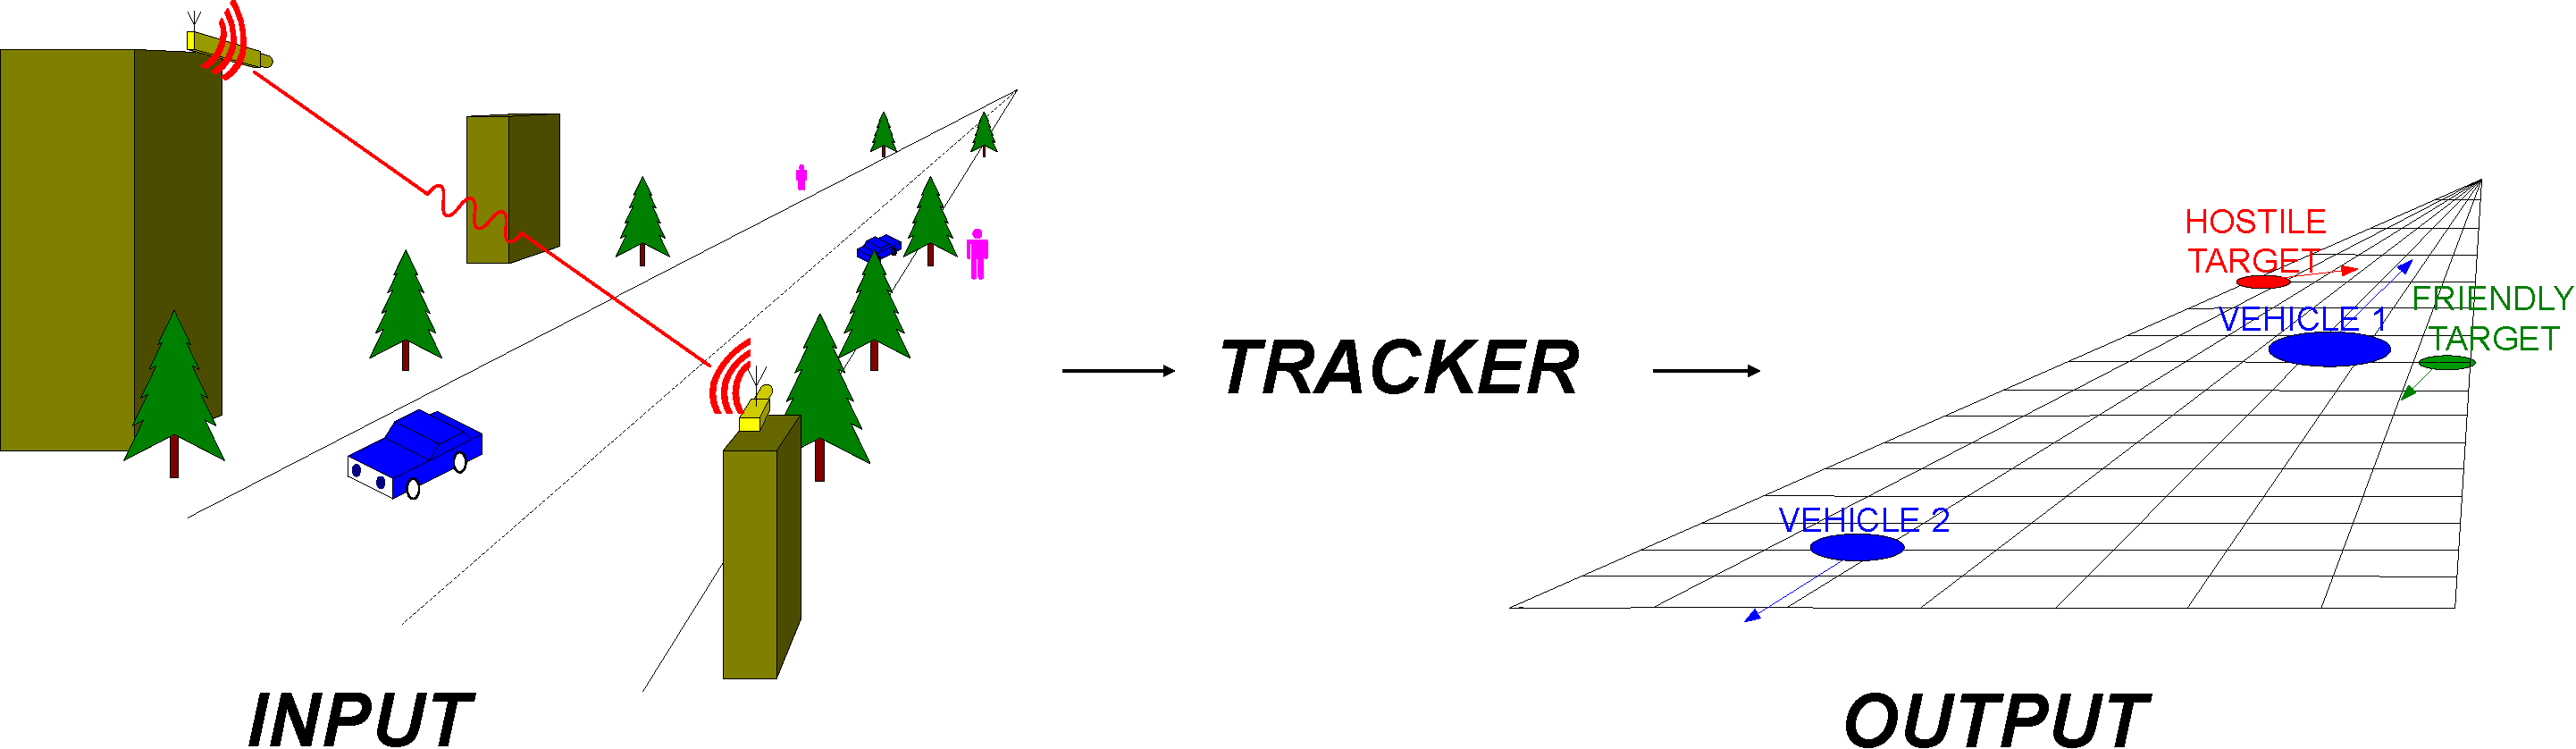
\includegraphics[width=1.1\textwidth]{figs/TRK_overviewDiagram.pdf}
	\caption{Illustration of a visual tracking scenario.}
	\label{fig:TRK_illustration}
\end{figure}

Recently, there has been a surge in interest in tracking due to several reasons: (a) proliferation of powerful computers, (b) availability of high quality and inexpensive video cameras, and (c) an increasing need for automated video analysis.  However, many practical difficulties are encountered during multi-target visual-tracking.  Some of these challenges include, 

\begin{itemize}
\item Loss of information caused by projecting 3D world objects onto 2D images
\item Sudden illumination changes
\item Appearance drifts
\item Complex target motion, including acceleration
\item Non-rigid or articulated nature of objects
\item Object-to-object merges/splits/occlusions
\item Object-to-scene occlusions
\item Camera motion
\item Noise
\item Real time processing requirements
\end{itemize} 

Clearly, visual tracking is a challenging problem.  Under general conditions, it remains an unsolved problem.  Several researchers have tried to approach this problem by specifying additional constraints on the targets being tracked.  Constraints have also been placed on the tracking environment.  For example, almost all tracking algorithms assume that the object motion is smooth without any abrupt changes \cite{2006_JNL_SURVEYtrk_Yilmaz}.  Furthermore, prior knowledge about the number, size, appearance and shape of the tracked objects has been used to simplify the problem.  

\begin{figure}[t]
	\center
	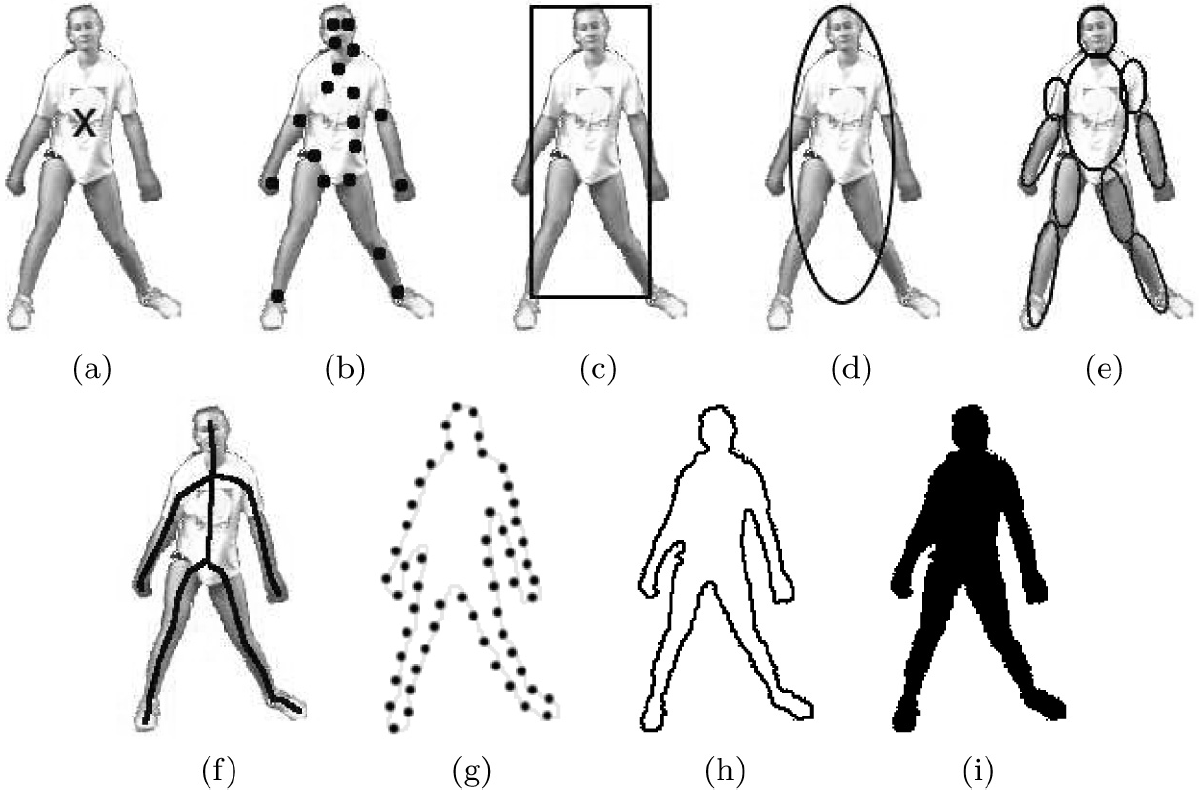
\includegraphics[width=1.0\textwidth]{figs/2006_JNL_TRKsurvey_Shah_fig1.png}
	\caption{Target representations.  (a) Centroid, (b) multiple points,(c) rectangular bounding box, (d) elliptical bounding region, (e) articulated shape model, (f) skeleton, (g) contour control points, (h) contour, (i) silhouette \cite{2006_JNL_SURVEYtrk_Yilmaz}.}
	\label{fig:TRK_objectRepresentations}
\end{figure}

A graphical illustration of the tracking problem is shown in Figure~\ref{fig:TRK_illustration}.  In this figure, multiple cameras are employed for visual surveillance in an outdoor scenario.  The images captured by these cameras are fed to a tracker which returns metadata about the objects being tracked, such as target ID and target velocity.  Tracking is also commonly used in indoors applications, such as in tracking people in airports and malls.  Single camera tracking is also still widely used although multi-camera tracking is an active area of research.

%#################################
\section{Solutions}
%#################################
In the preceding section, we outlined the tracking scenario and some challenges faced therein.  We now turn to solutions.  

%===================
\subsection{Target representations}
%===================
Several algorithms have been employed for single and multiple target tracking.  The nature of the algorithm chosen is closely tied to the target representation.  Several target representations are shown in Figure~\ref{fig:TRK_objectRepresentations}.  

%===================
\subsection{Tracking algorithms}
%===================
The different target representations shown in Figure~\ref{fig:TRK_objectRepresentations} lend themselves to the following general categories of trackers:

\begin{itemize}
\item \underline{Point tracker}.  Targets represented using centroids or multiple points are commonly tracked using point trackers.  This form of tracking is closely tied to radar tracking.  As a matter of fact, the same techniques used in radar tracking are used.  Commonly used techniques include Kalman filters, particle filters and the Probabilistic Data Association Filter (PDAF) \cite{1983_JNL_JPDAF_Fortmann}.
\item \underline{Region tracker}.  Targets represented using bounding boxes are commonly tracked using region tracking.  Widely used tracking methods in this category are template matching and mean shift tracking \cite{2002_JNL_MeanShift_Comaniciu}.
\item \underline{Contour tracker}.  Targets represented using shape information are commonly represented using splines and tracked using active contours \cite{2000_BOOK_ActiveVision_Blake} and level sets \cite{1995_JNL_LevelSets_Malladi}.
\end{itemize}

A closely associated problem is that of data association.  An overview of data association methods in target tracking is given in \cite{1993_JNL_SURVEYcorresp_Cox}.  More recently, particle filters have been shown to have an inherent capacity for data association \cite{1998_JNL_Condensation_IsardBlake}.   

%===================
\subsection{Preprocessing}
%===================
\begin{figure}[t]
	\center
	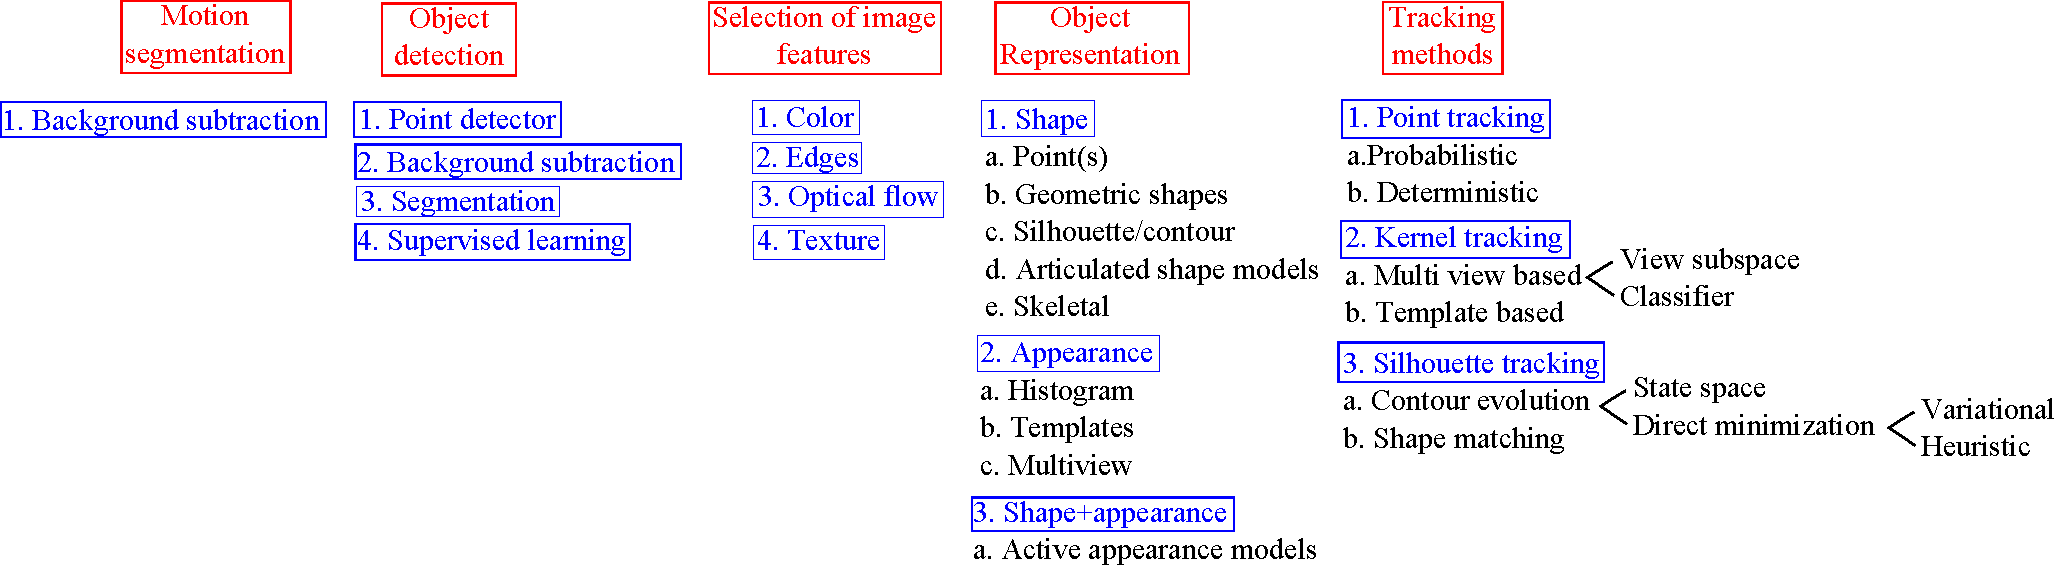
\includegraphics[width=1.15\textwidth]{figs/TRK_overview.pdf}
	\caption{Visual tracking pre-processing steps, object representations and tracking methods adapted from \cite{2006_JNL_SURVEYtrk_Yilmaz}.}
	\label{TRK_overviewDiagram}
\end{figure}


It is common to apply pre-processing steps before tracking is initiated.  Some of these techniques include 

\begin{itemize}
\item \underline{Downsampling}.  This step is commonly carried out to reduce computational complexity.
\item \underline{Normalization}.  This step is commonly used to normalize brightness variation in temporal sequences.
\item \underline{Stabilization}.  Camera jitter is a common problem in tracking, especially in outdoor scenarios, or where cameras are hand-held.  Different camera stabilization algorithms have been proposed to reduce the effect of camera motion.  An overview can be found in \cite{2006_WHITE_stab_Sachs, 1999_JNL_stab_Engelsberg}
\item \underline{Background modeling}.  Several methods have been suggested for background modeling.  A commonly used method is the Multi-gaussian algorithm \cite{1999_CNF_RealTimeTracking_Stauffer}.  An overview of background modeling methods can be found in \cite{1999_CNF_Wallflower_Toyama}.
\item \underline{Feature extraction}.  It is common to extract features from the target of interest and apply the algorithms mentioned above in the feature domain rather than the raw spatial domain.  Commonly used features include color, edges, corners, motion, texture, depth and spatial intensity probability distribution.  For instance, corner detection \cite{1988_CNF_CombinedCornerEdgeDetector_Harris,2004_JNL_SIFT_Mikolajczyk} can be used to extract points of interest within the target which are then tracked using point trackers. 
\end{itemize}

An overview of these pre-processing steps, different object representations, and tracking methods is given in Figure~\ref{TRK_overviewDiagram}.

%#################################
\section{Current work}
%#################################
In this work, we use a technique called Residual Vector Quantization (RVQ) for tracking.  This technique is explained in detail in Chapter~\ref{chap_RVQ}.  In this introductory chapter, we just mention that RVQ has been in use in the signal processing community since 1982 \cite{1982_CNF_SpeechRVQ_JuangGray} when it was introduced for speech compression.  Even today, this method is still mainly used in speech processing.  The first application of RVQ for image analysis was in 2007 \cite{2007_JNL_IDDM_Barnes} where it was used to analyze damage caused by Hurricane Katrina in 2005 and the Sri Lankan Tsunami in 2007.  As of today, only two journals and less than 10 conference papers exist on the usage of RVQ for image analysis.  We build on this and present the first usage of RVQ for video analysis.  The two use cases we use are visual recognition and visual tracking.  The main emphasis however, is placed on visual tracking.

%#################################
\section{Outline}
%#################################
So far, we've briefly discussed three things in this introductory chapter: (a) the problem that we attempt to solve in this work, (b) the methods that have been employed in an attempt to solve this problem, and (c) the method that we intend to use in our own attempts.  The remaining portion of this document elaborates on these issues.  Here is an outline:

\begin{itemize}
\item \underline{Chapter 2.  Residual Vector Quantization}.  In this chapter, we discuss RVQ, give the mathematical notation involved, and discuss design, optimality and implementation issues.  A comparison with other vector quantization methods is also given.
\item \underline{Chapter 3.  RVQ in computer vision (recognition)}.  In this chapter, we first show that it is possible to use RVQ for face recognition.  We then turn to using RVQ for action recognition in image sequences.  We build on this transition to employ RVQ for tracking in the next chapters.
\item \underline{Chapter 4.  Tracking methods}.  In this chapter, an overview of existing tracking methods is given before usage of RVQ in tracking is introduced in the next chapter.
\item \underline{Chapter 5.  RVQ in computer vision (tracking)}.  This is the most detailed chapter and builds on the groundwork laid in earlier chapters in an attempt to solve the visual tracking problem.  We compare RVQ tracking with two existing well known methods, PCA (Principal Components Analysis) tracking and TSVQ (Tree Structured Vector Quantization) tracking.  Seven different datasets are used that cover a variety of scenarios including indoors, outdoors, day-time, night-time, human, vehicle and object tracking, rigid and non-rigid object tracking, lighting change, structured noise, camera motion, target pose and expression changes, and temporary occlusions.  Results for over ten thousand hours of simulations are presented and analyzed.
\item \underline{Chapter 6.  Conclusions}.  This chapter wraps up this thesis briefly restating objectives, summarizing results, presenting conclusions and laying out a ground map for future work.
\end{itemize}











%@@@@@@@@@@@@@@@@@@@@@@@@@@@@@@@@@@@@@@@@@@@@@@@@@@
\chapter{RVQ (Residual Vector Quantization)}
\label{chap_RVQ}	
%@@@@@@@@@@@@@@@@@@@@@@@@@@@@@@@@@@@@@@@@@@@@@@@@@@

\begin{figure}[htp]			
	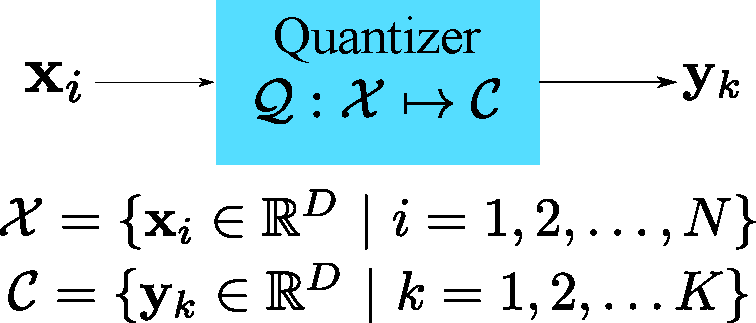
\includegraphics[width=1\textwidth]{thesis/Quantization_blockDiagram.pdf}
	\caption{A quantizer $Q$ maps symbols from a source alphabet $\mathcal{X}$ to symbols from a reconstruction alphabet $\mathcal{C}$, where in general, the number of elements in $\mathcal{C}$, $|\mathcal{C}| << |\mathcal{X}|$, the number of elements in $\mathcal{X}$ }
	\label{fig:Quantization_block_diagram}
\end{figure}

%####################
\section{Quantization}
%####################
%====================
\subsection{Introduction}
\label{sec:quantization}
%====================

The main mechanism for achieving lossy compression in images and videos is the process of \emph{quantization}.  For instance, all current video standards, MPEG-1, MPEG-2, MPEG-4, H.261, H.263 and H.264 rely on a special form quantization called \emph{transform vector quantization}, for compression.  Quantization is the process of representing a large, possibly infinite, set of values with a smaller set of values.  Figure~\ref{fig:Quantization_block_diagram} shows a quantizer $Q$ that takes values from a source alphabet $\mathcal{X}$,

\begin{equation}
\mathcal{X}=\{x \in \mathcal{R}^D\}
\end{equation}

and maps them to a reconstruction alphabet $\mathcal{C}$, 

\begin{equation}
\mathcal{C}=\{\mu_k \in \mathcal{R}^D | k=1,2, \ldots K\}
\end{equation}

The $K$ partitions $P_k, k = 1, 2, \ldots, K$ created in the input space $R^D$, 

\begin{equation}
P_k = \{x \in R^D | Q(x) = \mu_k\}
\end{equation}   

are mutually exclusive,

\begin{equation}
P_i \bigcap P_j = \emptyset, \ i \neq j
\end{equation}

and the union of these partitions covers the entire input space,

\begin{equation}
\bigcup\limits_{k=1}^{K} P_k=\mathcal{R}^D
\end{equation}

The reconstruction alphabet is also known as the \emph{codebook}.  Members of this set, $\mu_k$ are called \emph{codevectors}.  If the input is scalar, i.e. $D=1$, the quantizer is called a \emph{scalar quantizer} (SQ).  For $D>1$, the quantizer is called a \emph{vector quantizer} (VQ).  The \emph{resolution}, \emph{code rate}, or simply the \emph{rate} $r$ of a quantizer, 


\begin{figure}[t]			
	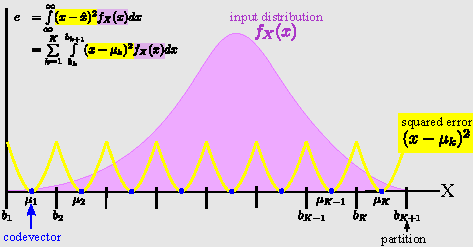
\includegraphics[width=1\textwidth]{thesis/Quantization_MSE.pdf}
	\caption{Computing optimal centroids.}
	\label{fig:computing_optimal_centroids}	
\end{figure}

\begin{equation}
r=\frac{\log_2 K}{D}
\end{equation}  

is proportional to the number of bits required to represent the total number of codevectors, $K$ and inversely proportional to the dimensionality of the data.  This shows that for the same number of codevectors $K$, the rate increases linearly with the dimensionality of the data.  VQ is therefore able to achieve higher rates than SQ.  However, for a given error metric $d(.)$, a common one being the squared error criterion, 

\begin{equation}
d(x,y)=(x-y)^2 
\end{equation}

higher rates can increase distortion $\mathcal{D}$,

\begin{equation}
\mathcal{D(\mathcal{X}, \mathcal{C})} =E\left[d(x, Q(x)) \right]
\end{equation}

This tradeoff between rate and distortion can be plotted to create a \emph{rate-distortion} curve.  A fundamental result of Shannon's rate-distortion theory is that VQ will always achieve equal better or equal compression rates than SQ, even if the source is memoryless, i.e., emits a sequence of IID random variables \cite{1984_JNL_VQ_Gray}.   The reason is that SQ quantizes each dimension separately and cannot therefore exploit statistical correlation between the different dimensions of the data.  The result is rectangular partitions $P_k$ in $R^D$.  On the other hand, VQ can carve up the input space into arbitrary shapes.

\begin{figure}[t]		
	\center	
	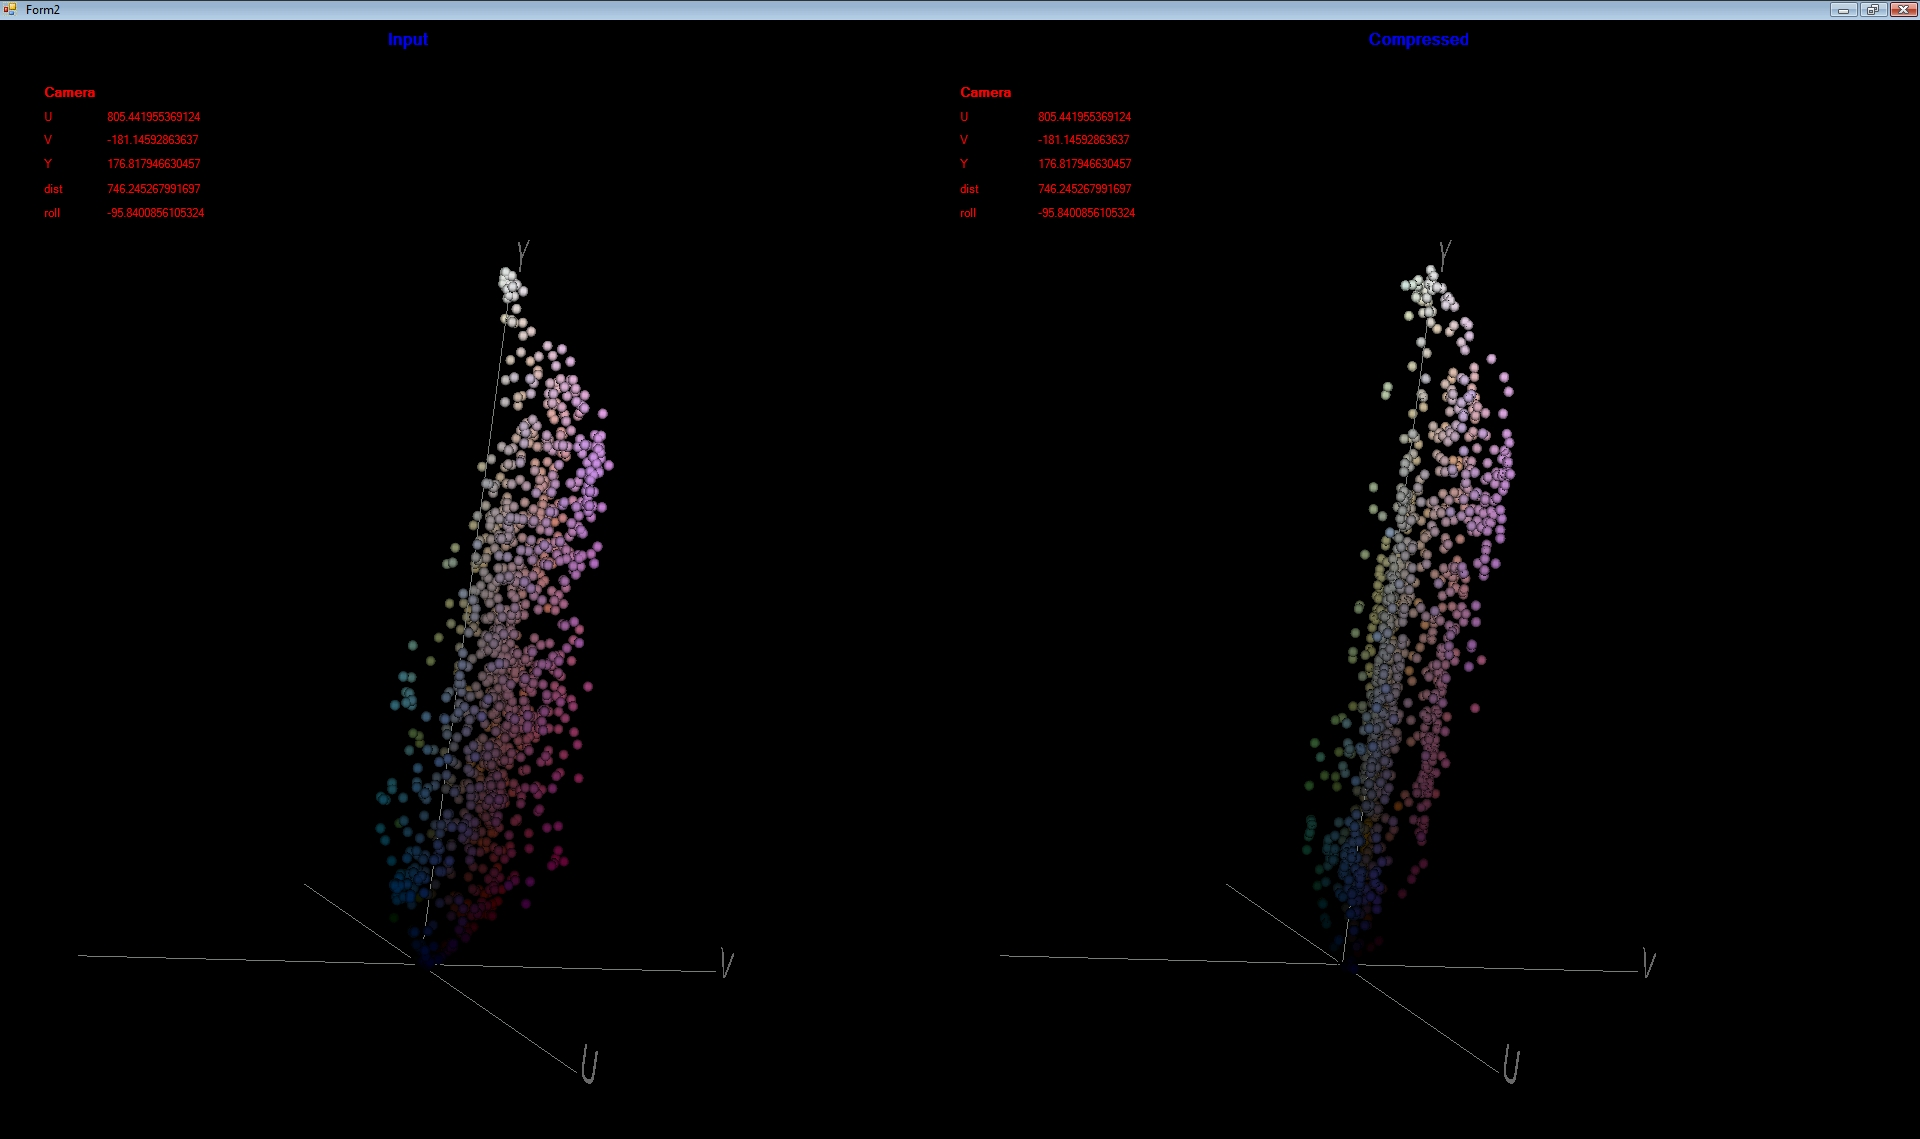
\includegraphics[height=0.4\textheight]{thesis/MPEG4_VTK.png}
	\caption{Scalar quantization in the transform domain for MPEG-4.  The image on the left shows the 3 intensity channels of an input image patch drawn in the YUV color space.  The vertical dimension is the luma (Y) axis.  The right image shows the quantized reconstruction of the input image patch.  No deblocking filter has been used, and so the loss of information is entirely due to quantization.  Notice the straight lines along which the output pixels are aligned due to the quantization process.  The visualization was created using the Visualization Toolkit (VTK) \cite{VTK} in C.}
	\label{fig:MPEG4_VTK}
\end{figure}


%====================
\subsection{Optimality issues}
%====================
\begin{figure}[t]		
	\center	
	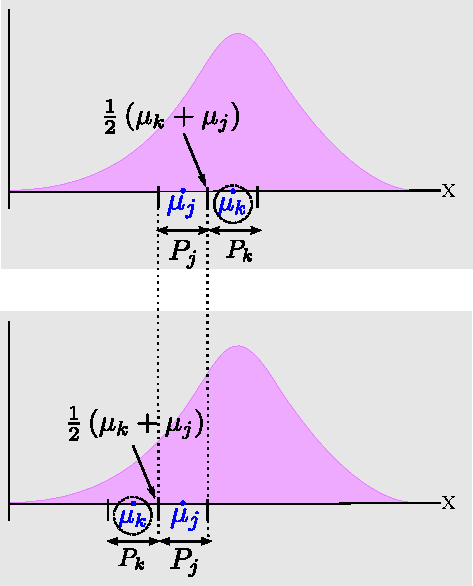
\includegraphics[height=0.5\textheight]{thesis/Quantization_optimalPartitions2.pdf}
	\caption{Computing optimal partitions}
	\label{fig:computing_optimal_partitions}
\end{figure}

So far, no mention has been made about optimality of the codevectors or partitions.  A widely used algorithm to compute optimal codevectors and partitions is the Generalized Lloyd Algorithm (GLA) \cite{1991_BOOK_VQ_GershoGray}, also known as the Linde Buzo Gray (LBG) algorithm \cite{1982_JNL_LeastSquaresQuantization_Lloyd} or K-means clustering \cite{1967_CNF_Kmeans_Macqueen}.  Figure~\ref{fig:computing_optimal_centroids} illustrates the SQ case for an input $X$ with distribution $f_X(x)$ and squared error criterion, 

\begin{equation}
e=\sum\limits_{k=1}^{N} \int\limits_{b_k}^{b_{k+1}}(x-\mu_k)^2f_X(x)
\end{equation}

If the partitions $P_k$,

\begin{equation}
\label{Eq:partitions}
P_k =  \left\{x \ | \ (\mu_j-x)^2 < (\mu_k-x)^2, \ \forall \ j \neq k \right\}
\end{equation}

are given, an optimal codevector $\mu_k$ can be computed by setting the derivative of the error $e$ with respect to $\mu_k$ equal to 0,

\begin{equation}
\frac{\partial{e}}{\partial{\mu_k}} = 0
\end{equation}

In other words, the optimal centroid for a given partition and the squared error criterion is the centroid of the partition. 

\begin{equation}
\mu_k = \frac
{\int\limits_{b_k}^{b_{k+1}}xf_X(x)dx}
{\int\limits_{b_k}^{b_{k+1}}f_X(x)dx}
\end{equation}

To compute optimal partitions, given the centroids, we can rewrite Equation~\ref{Eq:partitions} as 

\begin{equation}
\label{Eq:partitions2}
P_j=\left\{x \ | \ (\mu_k -\mu_j) \left(x - \frac{1}{2} \left(\mu_k + \mu_j \right)\right) < 0, \ \forall j \neq k 
\right\}
\end{equation}

For the scalar case in Figure~\ref{fig:computing_optimal_partitions}, if $k>j$, i.e. $(\mu_k -\mu_j) > 0$, then to satisfy Equation~\ref{Eq:partitions2}

\begin{align}
\label{Eq:partitions3}
x - \frac{1}{2} \left(\mu_k + \mu_j \right) &< 0\notag\\
\Rightarrow x &< \frac{1}{2} \left(\mu_k + \mu_j \right)
\end{align}

Conversely, if $k<j$, i.e. $(\mu_k -\mu_j) < 0$, then to satisfy Equation~\ref{Eq:partitions2}

\begin{align}
\label{Eq:partitions4}
x - \frac{1}{2} \left(\mu_k + \mu_j \right) &> 0 \notag\\
\Rightarrow x &> \frac{1}{2} \left(\mu_k + \mu_j \right)
\end{align}

The only way to satisfy both Equations~\ref{Eq:partitions3} and \ref{Eq:partitions4} is for the partition boundary to be half-way between the centroids, , i.e. $\frac{1}{2} \left(\mu_k + \mu_j \right)$.  This notion can be generalized to the vector case.

%=================
\subsection{Types of VQ}
%=================
\begin{figure}[htp]				
	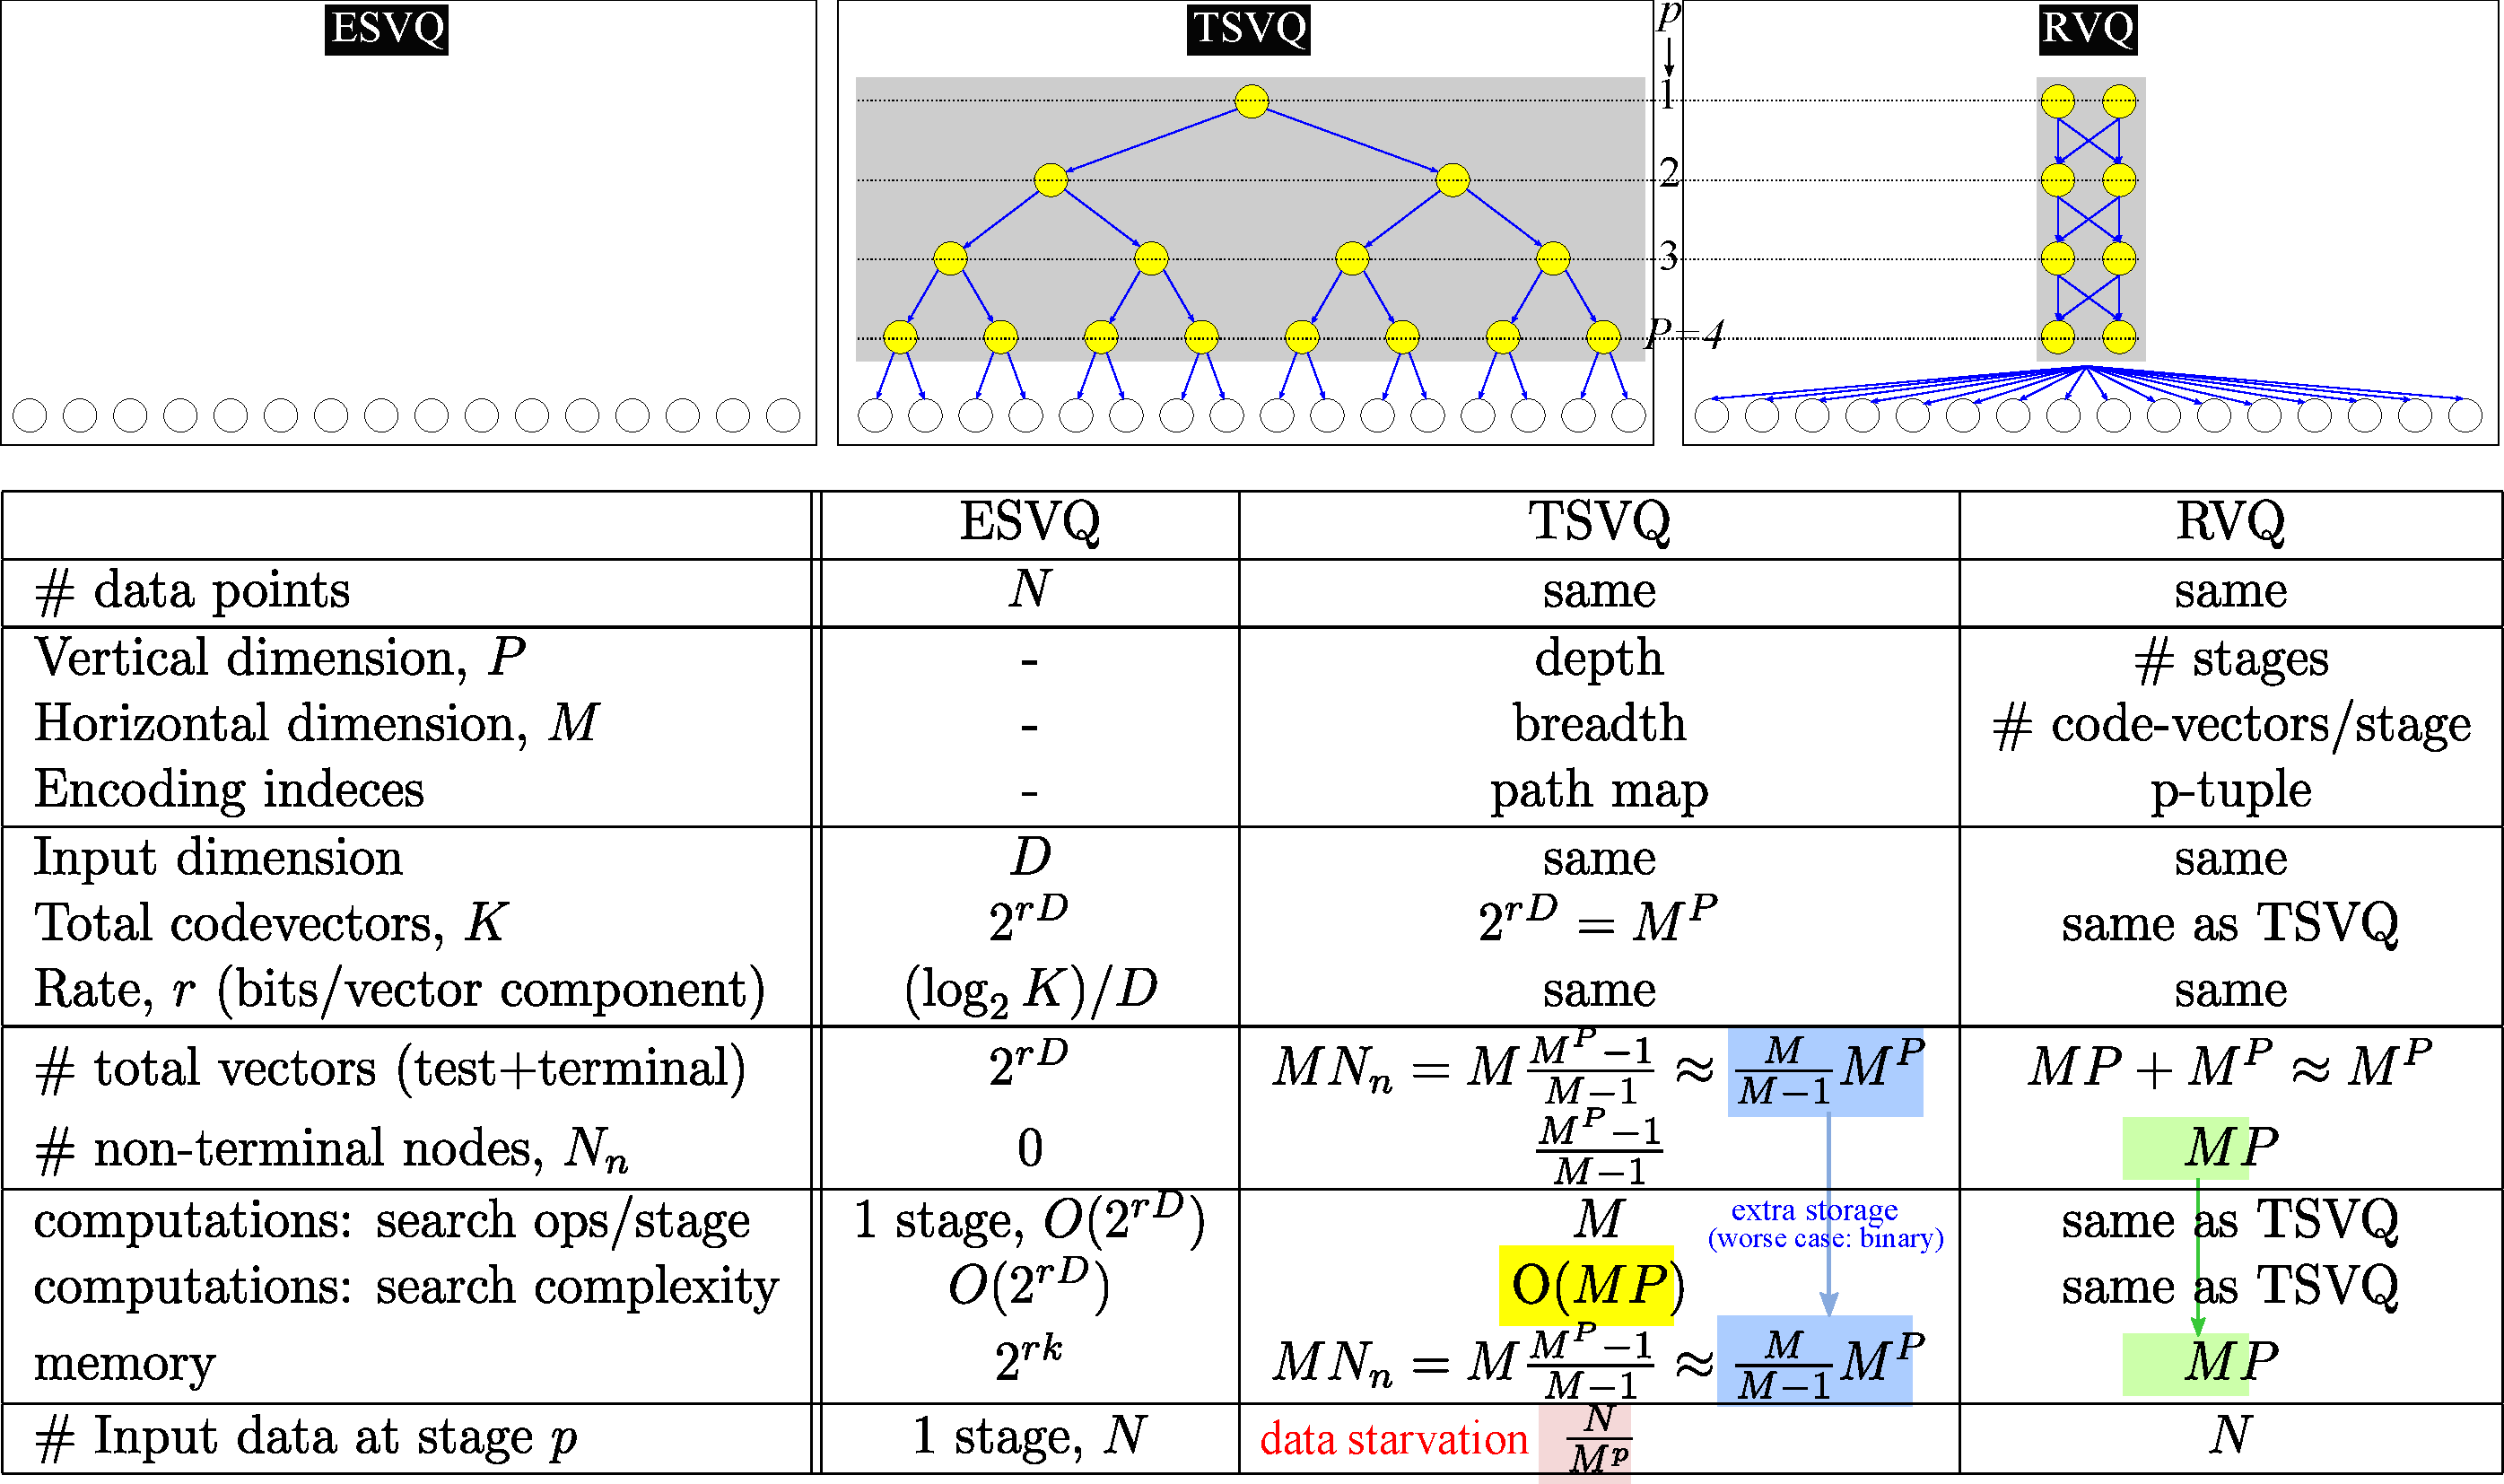
\includegraphics[width=1.1\textwidth]{thesis/RVQ_comparisonWithESVQ_TSVQ.pdf}
	\caption{Graphical comparison of ESVQ, TSVQ and RVQ, 16 codevectors}
	\label{fig:comparison_ESVQ_TSVQ_RVQ}
\end{figure}

\begin{table}[htp]
\begin{longtable}{| p{2.2in} || p{1in} | p{1.5in} | p{1.5in}|}
\hline
											&ESVQ						&TSVQ																&RVQ								\\ 
\hline
\# data points								&$N$						&same																&same								\\ 
\hline
Vertical dimension, $T$					&-							&depth																&\# stages							\\
Horizontal dimension, $M$					&-							&breadth															&\# templates						\\
Encoding indeces							&-							&path map	(T-tuple)												&XDR (T-tuple)						\\ 
\hline
Input dimension							&$D$						&same																&same								\\
Rate, $r$ (bits/vector component)			&$(\log_2K)/D$			&same																&same								\\ 
\hline
\# non-terminal codevectors, $N_{ntc}$	&0							&$1+M+M^2+ \ldots + M^{T-1}=\frac{M^T-1}{M-1}$			&$MT$								\\
\# terminal codevectors, $K$				&$2^{rD}$					&$2^{rD}=M^T$													&same as TSVQ					\\
\hline
computations: search ops/stage			&1 stage, $O(2^{rD})$	&$M$																&same as TSVQ					\\
computations: search complexity 			&$O(2^{rD})$				&O($MT$)															&same  as TSVQ					\\ 
memory 									&$2^{rD}$					&$MN_{ntc} = M\frac{M^T-1}{M-1}\approx\frac{M}{M-1}M^T$ &$MT$								\\ 
\hline
\# Input data at stage $t$					&1 stage, $N$				&$\frac{N}{M^t}$													&$N$								\\
\hline
\end{longtable}
\caption{Comparison of ESVQ, TSVQ and RVQ}
\label{tab:comparison_ESVQ_TSVQ_RVQ}
\end{table}
We now list the main types of VQ that appear in the literature.  The goal of VQ design is to have output distortion as close as possible to the rate-distortion curve.  However, in general, optimal coding of source vectors is not possible unless an exhaustive search over all code-vectors is carried out, as in structurally unconstrained \emph{Exhaustive Search Vector Quantizers} (ESVQs) \cite{1992_JNL_RVQ_Barnes}.  For a rate $r$ and dimension $D$, there are $K=2^{rD}$ code-vectors.  The computational costs of $EVSQ$, $C_{ESVQ}$, and memory requirements $M_{ESVQ}$ are $\approx 2^{rD}$.  A solution to this problem is to impose constraints on the VQ structure.  One possible solution is the Tree Structured VQ (TSVQ) proposed in \cite{1980_JNL_TSVQ_Buzo}.  A $T$-level, $m$-ary TSVQ has search complexity $C_{TSVQ} \approx mT$ but double storage requirements, $M_{TSVQ} \approx 2 M_{ESVQ}$.   So, although the $TVSQ$ solves the search complexity problem, it further aggravates the storage problem.  A method of reducing both computational and storage complexity is to use a product code VQ.  The basic idea in a product code VQ is to break a bigger problem into several smaller problems.  Examples include mean-residual VQ, gain-shape VQ and mean-gain-shape VQ \cite{1996_JNL_AdvancesRVQ_Barnes}.  Residual Vector Quantizers (RVQ) also fall under this category, and are of interest to us in this work.  A comparison of ESVQ, TSVQ and RVQ is given in Table~\ref{tab:comparison_ESVQ_TSVQ_RVQ}.  A graphical comparison with 16 codevectors is given in Figure~\ref{fig:comparison_ESVQ_TSVQ_RVQ}.

%####################
\section{RVQ}
%####################
Residual Vector Quantizers were introduced by Juang et al. \cite{1982_CNF_SpeechRVQ_JuangGray}.  The RVQ structure is shown in Figure \ref{fig:RVQ_block_diagram}.  Initially a crude quantization of the input vector is carried out using a small codebook.  Then a second stage quantizer operates on the error of the first quantizer.  A third quantizer may be used to quantize the second error vector, and so on.  In other words, RVQs are realized as a sequence of small ESVQs.  Each stage operates on the error vector or \emph{residual} of the preceding ESVQ \cite{1991_CNF_DesignPerformanceRVQ_Frost}.  This direct sum structure coupled with a sequential search procedure enables the RVQ to have linear rather than exponential complexity, both in computations and in memory.  Two alternate graphical representations of this direct sum structure are given in Figure~\ref{fig:RVQ_sigma_tree}.

\begin{figure}				
	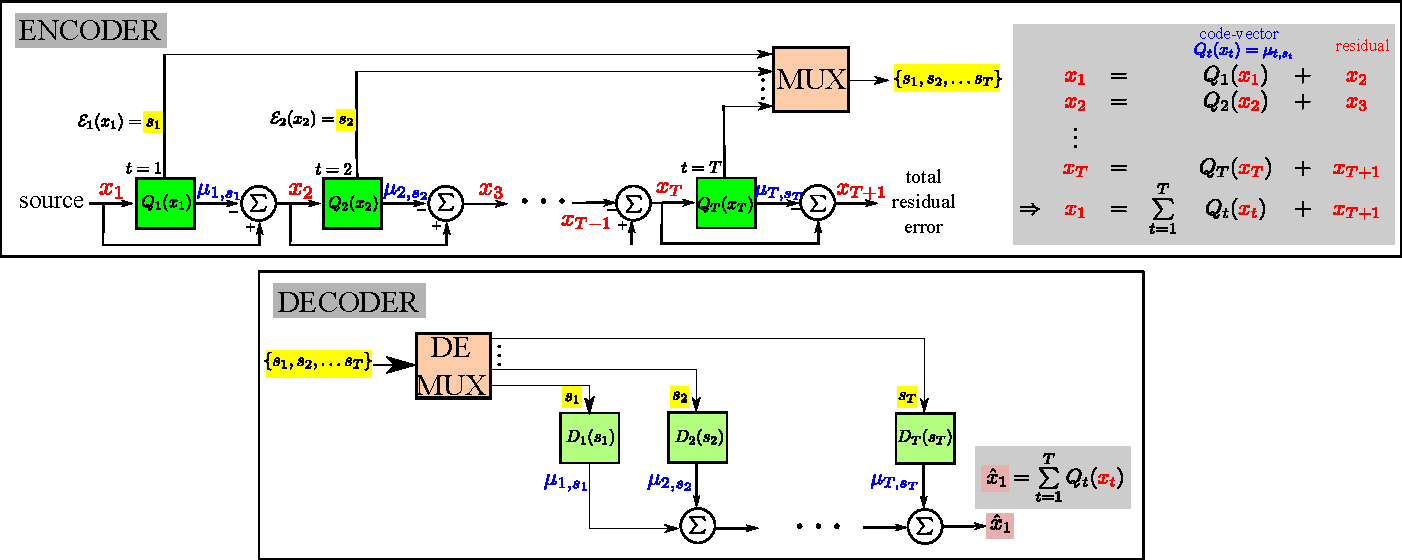
\includegraphics[width=1\textwidth]{thesis/RVQ_blockDiagram.pdf}
	\caption{RVQ: block diagram}
	\label{fig:RVQ_block_diagram}
\end{figure}

An RVQ is different from a traditional VQ in the sense that it partitions the input space $R^D$ into $M$ cells.  The residual space, also in $R^D$, is then partitioned again into $M$ cells.  This process is repeated $T$ times.  The advantage of this approach is that in obtaining $M^T$ partitions, we need to run our partitioning algorithm $T$ times and generate $M$ partitions at each stage.  In traditional VQ, the partitioning algorithm would run once but have to create $M^T$ partitions.  For the binary case (two code-vectors per stage, $M=2$) and a total of 8 stages ($T$=8), RVQ only requires 16 searches.  In $ESVQ$, this would require 256.  The exponential complexity is reduced to linear complexity.  Moreover, even the distortion of an ESVQ can be attained.  In general, all structurally constrained quantizers cannot provide performance as good as ESVQ.  However, since they are able to more efficiently implement codes, larger and larger vector sizes can be used, and if carefully designed, can achieve better performance that ESVQ \cite{1996_JNL_AdvancesRVQ_Barnes}.

\begin{figure}[ht]
	\centering	
	\subfigure[]
	{
		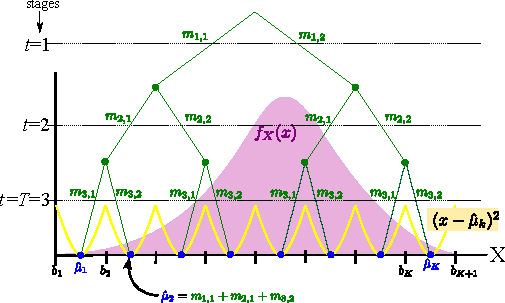
\includegraphics[width=0.65\textwidth]{thesis/RVQ_graphicalReconstruction.pdf}
		\label{fig:MTT_codebooks}	
	}
	\subfigure[]
	{
		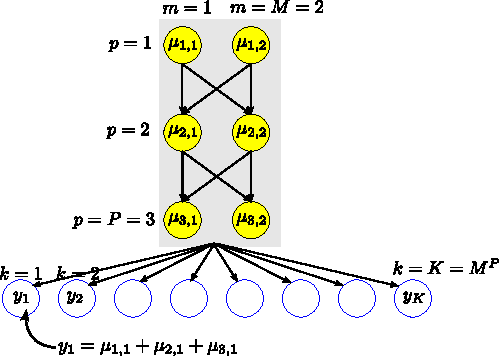
\includegraphics[width=0.65\textwidth]{thesis/RVQ_trellis.pdf}
		\label{fig:MTT_reconstruction}	
	}
	\caption{RVQ $\sigma$-tree, $T$=3, $S=2$, two alternate representations} 
	\label{fig:RVQ_sigma_tree}				
\end{figure}


%=======================
\subsection{Encoder}
%=======================
A vector quantizer with a direct sum codebook,

\begin{itemize}
\item is the source coding dual of a $\sigma$-tree structure \cite{1993_sigmaTrees_Barnes}, and
\item its design is the covering design problem
\end{itemize}

Since the dual of the covering problem is the packing problem \cite{BOOK_spheres_Conway}, it is shown in \cite{1993_sigmaTrees_Barnes} that $\sigma$-tree structures exist that provide good packing.  The design of RVQ direct sum codebooks is therefore studied in the context of $\sigma$-trees.

The set $\mathcal{S}$ of $K$ leaf nodes of a $T$-level $M$-ary $\sigma$-tree is the set of $M^T$ direct sums of $T$ vectors in $R^D$, one vector per level $t$ being picked from a \emph{constituent set} $G_t = \{m_{t,m} \in R^D \ | m=1, 2, \ldots M\}$ \cite{2002_JNL_SigmaTrees_Barnes},

\begin{equation}
\mathcal{S} = \{\hat{\mu}^{(k)} \in R^D \ | \ \hat{\mu}_k = \sum\limits_{t=1}^T m_t^{(k)}, k=1, 2, \ldots, K=M^T\}
\end{equation}

An example 3-level binary $\sigma$ tree is given in Figure~\ref{fig:RVQ_sigma_tree}.  The RVQ encoder can be designed in two major phases which are explained below and illustrated in Figure~\ref{fig:RVQ_encoder_flowDiagram}. 
 


 

\begin{figure}[ht]
\centering
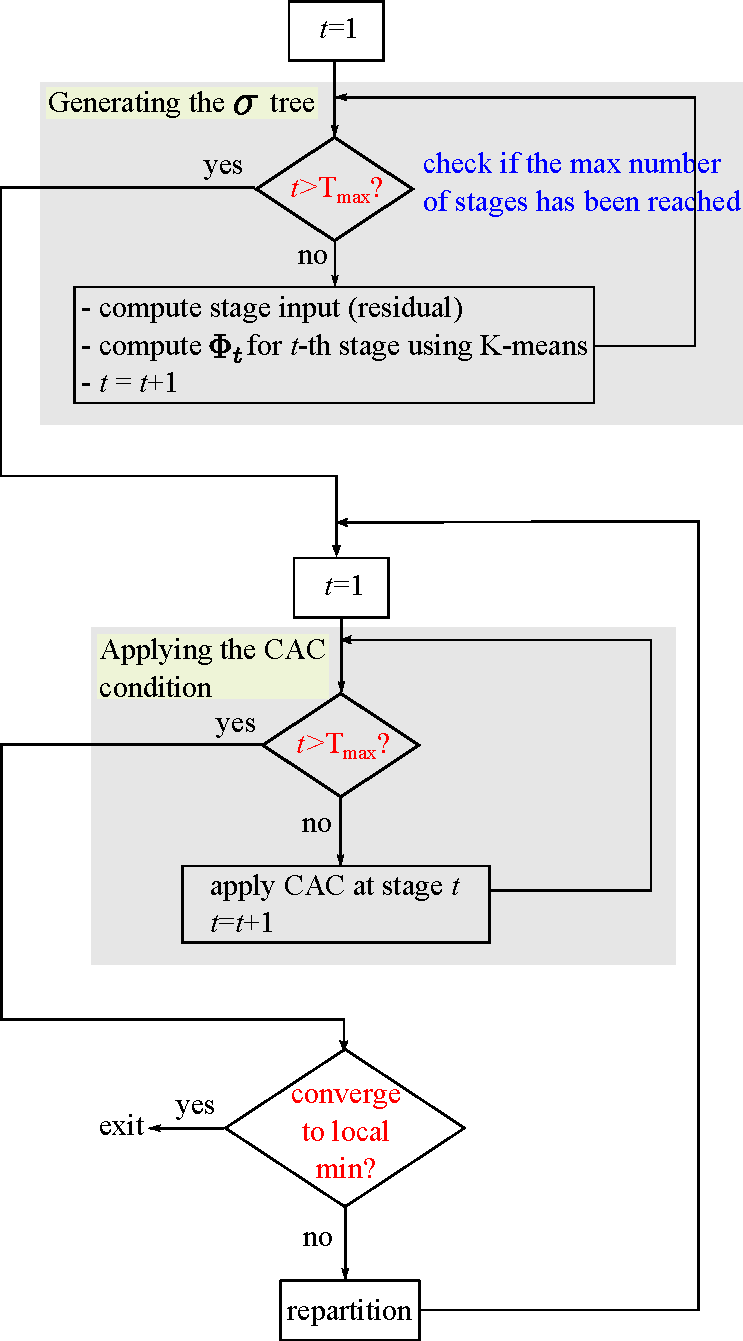
\includegraphics[height=0.6\textheight]{thesis/RVQ_encoder_flowDiagram.pdf}
\caption{Encoder flow diagram, generating codebooks $\Phi$}
\label{fig:RVQ_encoder_flowDiagram}
\end{figure}


\begin{enumerate}
\item \underline{Generating the $\sigma$ tree}.  The first design step is to generate the RVQ $\sigma$-tree by repeated application of the K-means algorithm to every stage in the following manner:  
\begin{enumerate}
\item \underline{First stage}. As in the K-means algorithm, standard practice is to generate several arbitrary partitionings and to retain the partition that results in least error as given by Equation~\ref{Eq:computingClusterCentroids}.  The objective function for the discrete case is,

\begin{equation}
\label{Eq:KmeansError}
e = \KmeansError
\end{equation}

The means of this partitioned data constitute the first stage codevectors.  In effect, this step generates $S$ stage codevectors, where typically, $S << K$.  For instance, if $K=16$ clusters are desired in ESVQ, RVQ can attain that many clusters with say $T=4$ stages and $S=2$ codevectors per stage.  Notice that in this equation, it is implicit that the partitions are known.  The outer summation that sums over the $K$ clusters is what makes this an NP hard problem, otherwise this would be a standard least squares problem.  Once the partitions are fixed, this can be solved as a standard least squares problem by setting the derivatives equal to 0.  

\begin{align}
\frac{\partial{e}}{\partial{\mu_k}} &= 0\notag\\
\KmeansInnerSum 2 \KmeansInner &= 0\notag\\
\KmeansInnerSum x_i - \KmeansSum \mu_k &= 0\notag\\
\KmeansInnerSum x_i - N_k \mu_k &= 0\notag\\
\mu_k &= \frac{\KmeansInnerSum x_i}{N_k}
\label{Eq:computingClusterCentroids}
\end{align}

In the equation above, $\mu_k$ is the cluster centroid for the $k$-th partition $\mathcal{K}_k$.  Once the $K$ cluster centroids have been computed, the data is repartitioned.  In other words, data points are mapped to the nearest new cluster centroids.  The cluster centroids are recomputed using Equation~\ref{Eq:computingClusterCentroids}.  This process of partitioning followed by centroid computation followed by repartitioning followed by centroid computation is repeated till the centroids converge.

\item \underline{Generating residual stages}.  In the step above, stage codevectors are subtracted from the data points that map to them.  This step generates a new set of data points, the first stage \emph{residual} data points.  The data at the output of stage $t$ is called the $t$-th residual data.  This causes each cluster in the first stage to be centered around the origin and also causes each data point to move closer to the origin.  These residual data points are now input into the K-means algorithm which generates a new set of partitions and new cluster centroids.  Using the same procedure discussed earlier, second stage residuals are generated and input to the third stage.  This process is repeated till the desired number of stages.  This Markovian style design process generates the initial RVQ $\sigma$-tree trellis.  
\end{enumerate}
\item \underline{Applying the CAC condition}.  The above step generates cluster centroids that are locally optimal at every stage.  Morever, the design of each stage depends on the previous or causal stage designs but does not depend on subsequent or anti-casual stage designs.   This can lead to a propagation of reconstruction error.  No optimality claims can be made regarding this design process.  An attempt to address this is a joint design strategy, also known as the Causal Anti-causal (CAC) condition.  This is explained next.
\end{enumerate}

\begin{figure}
\center
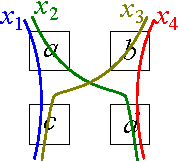
\includegraphics[width=0.5\textwidth]{thesis/RVQ_CAC_toyExample2_2x2.pdf}
\caption{2x2 RVQ example}
\label{fig:Figure1}
\end{figure}





\subsubsection{Causal Anti-causal condition}
%---------------------------------------------------
To understand CAC, it is beneficial to first introduce some notation:

\begin{itemize}
\item \emph{Path}.  A finite directed path through the RVQ $\sigma$-tree has as its vertices one stage codevector from every stage.  For $T$ stages and $S$ codevectors per stage, there are a total of $K = S^T$ possible paths.
\item \emph{Stage codevector}.  A stage codevector $m_{t, s}$ is the $s$-th codevector at the $t$-th stage.  An alternate notation used is $m^{(k)}_t$ which denotes the stage codevector at the $t$-th stage for the $k$-th path.
\item \emph{Optimal reconstruction}.  There are $K=S^T$ possible paths through the RVQ $\sigma$-tree.  Each data point $x_i$ propagates through the $\sigma$-tree on one of these $K$ paths.  If $x_i \mapsto \mathcal{K}_k$, then for optimal reconstruction, the following condition must hold true,

\begin{equation*}
\RVQunit = 0, \ \ \forall x_i \mapsto \mathcal{K}_k, \ \ i =1, 2, \ldots N\\
\end{equation*}

where $m^{(k)}_t$ is the stage codevector at the $t$-th stage of the $k$-th path through the $\sigma$-tree.  The above condition shows that

\begin{itemize} 
\item There are at most $K=S^T$ distinct data points that can result in 0 reconstruction error, irrespective of the dimensionality $D$ of the data. 
\item The non-Markovian reconstruction function produces a Direct Sum Successive Approximation (DSSA) of the input.
\end{itemize}\item \emph{Equivalent codevector}.  For every path through the RVQ $\sigma$-tree, we have an equivalent codevector $\hat{\mu}^{(k)}$ given by,
\begin{equation}
\hat{\mu}^{(k)} = \RVQequivalentCodevector, \ \ \ k=\{1, 2, \ldots, K\}
\end{equation}
In general, the $K$ equivalent codevectors and the accompanying $K$ partitions will approximate the $K$ cluster centroids and $K$ partitions produced by ESVQ.  The equivalent codevector can also be written as,
\begin{equation}
\label{Eq:RVQequivalentCodevectorBroken}
\hat{\mu}^{(k)} = \RVQequivalentCodevectorBroken
\end{equation}
\item \emph{RVQ objective function}.  The ESVQ objective function in Equation~\ref{Eq:KmeansError} can now be re-written in terms of the equivalent codevectors as 
\begin{equation}
e = \RVQerror
\end{equation}
\end{itemize}

Substituting for the equivalent codevector from Equation~\ref{Eq:RVQequivalentCodevectorBroken} gives

\begin{equation}
e=\KmeansSum{\bigg[\RVQmultipleKmeans\bigg]}^2, \ \ \tau=\{1, 2, \ldots T\}
\label{Eq:RVQmultipleKmeans}
\end{equation}

This equation states that for RVQ, the original objective function can be written as a series of coupled K-means equations, one equation per stage.    
 
\begin{align}
e&= \KmeansSum{\bigg[\RVQmultipleKmeansone\bigg]}^2, \ \ \tau=1\notag\\
&= \KmeansSum{\bigg[\RVQmultipleKmeanstwo\bigg]}^2, \ \ \tau=2\notag\\
&\ \ \ \  \ \ \ \vdots\notag\\
&=\KmeansSum{\bigg[\RVQmultipleKmeansT\bigg]}^2, \ \ \tau=T
\end{align}

Equation~\ref{Eq:RVQmultipleKmeans} can now be regrouped as,

\begin{align}
\label{Eq:RVQmeans}
e&= \KmeansSum{\bigg[\RVQmultipleKmeansonealternate\bigg]}^2, \ \ \tau=\{1, 2, \ldots T\}\notag\\
&={\RVQerroralternate}, \ \ \tau=\{1, 2, \ldots T\}
\end{align}

where $g_i$ is the \emph{graft residual} and is formed using the following steps,

\begin{itemize}
\item \emph{List all reconstruction stage codevectors in path}.  For a data point $x_i$, list all stage codevectors that are used to reconstruct it
\item \emph{Find graft residual at stage $\tau$}.  Subtract all stage codevectors in above step from $x_i$ except the stage codevector at the $\tau$-th stage  
 \end{itemize}

Equation~\ref{Eq:RVQmeans} is now quite clearly a K-means objective function for the $\tau$-th stage.  Here, $m_{\tau}^{(k)}$ is a single codevector at the $\tau$-th stage even though it has a superscript $k$ which tends to indicate that it might correspond to several codevectors.  The superscript $k$ refers to the fact that there are $K$ possible paths, but for a particular $g_i$, we choose the $m_{\tau}^{(k)}$ that lies in the reconstruction path of the corresponding $x_i$.  We can therefore rewrite Equation~\ref{Eq:RVQmeans} as,

\begin{equation}
e = \RVQOuterSum\RVQInnerSum\RVQinneralternatealternate
\end{equation} 

Now, to compute a particular stage codevector $m_{\tau, s}$, we use the standard GLA algorithm as in Equation~\ref{Eq:computingClusterCentroids} to get

\begin{equation}
m_{\tau, s} = \frac{\RVQInnerSum g_i}{N_{g_i \mapsto m_{\tau, s}}}
\label{Eq:finalCAC}
\end{equation}

\begin{figure}[ht]
\centering
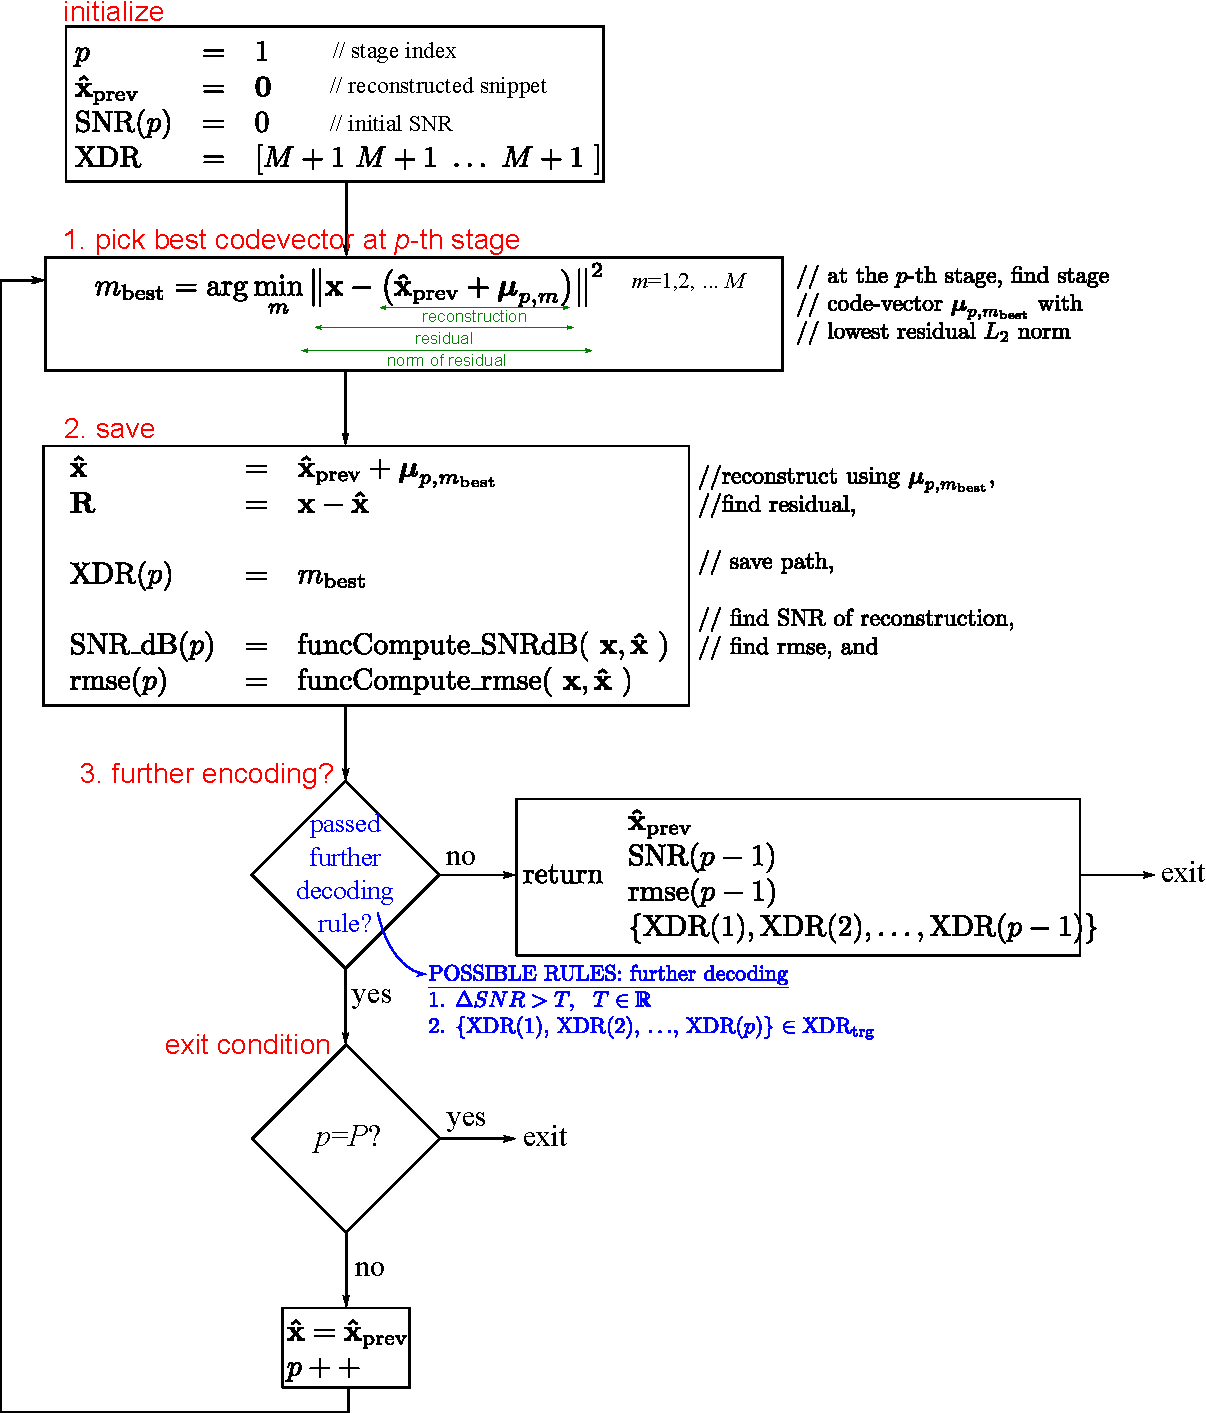
\includegraphics[height=0.6\textheight]{thesis/RVQ_explorer_flowDiagram.pdf}
\caption{Decoder flow diagram}
\label{fig:RVQ_decoderFlowDiagram}
\end{figure}


Equation~\ref{Eq:finalCAC} can now be used to compute the $S$ stage codevectors at the $\tau$-th stage.  $N_{g_i \mapsto m_{\tau, s}}$ is the number of graft residuals $g_i$ whose corresponding data points $x_i$ contain $m_{\tau, s}$ in their reconstruction path.  Recall that in ordinary K-means, computation of the centroids is followed by a repartitioning which is followed by a centroid computation and so on.  This process is repeated till convergence.  However, in this case of coupled K-means, two issues arise:

\begin{itemize}
\item repartitioning affects all stages.  
\item Moreover, recomputing the centroids for one stage changes the graft residuals for all other stages, since each graft residual depends on $S-1$ stage codevectors.  
\end{itemize}

Since RVQ update strategies are not the focus of this research, the reader is referred to  \cite{1996_JNL_AdvancesRVQ_Barnes} for more details.  The result of these steps is an RVQ codebook with $K$ codevectors,

\begin{equation}
\mathcal{M} = \{\hat{\mu}_1, \hat{\mu}_2, \ldots, \hat{\mu}_K\}
\end{equation}

Figure~\ref{fig:Figure1} shows a simple example of a 2x2 RVQ with 4 input data points.  The error is given by



\begin{equation}
\begin{array}{lllll}
e &=& \KmeansError \\
&=& {(x_1 - a - c)}^2 + {(x_2- a - d)}^2 + {(x_3 - b - c)}^2 + {(x_4 - b - d)}^2\\
&=& {e_1}^2 + {e_2}^2 + {e_3}^2 + {e_4}^2
\end{array}
\end{equation}

Applying the CAC condition to optimize stage 1, we get the following equations by grouping all input data points with stage codevectors that do not belong to stage 1,

\begin{equation}
\begin{array}{lllll}
e &=& {((x_1 - c) - a)}^2 + {((x_2- d) - a)}^2 + {((x_3 - c) - b)}^2 + {((x_4 - d) - b)}^2
\end{array}
\label{Eqn:2x2RVQ_stage1}
\end{equation}

And similarly, to optimize stage 2, we get,

\begin{equation}
\begin{array}{lllll}
e &=& {((x_1 - a) - c)}^2 + {((x_2- a) - d)}^2 + {((x_3 - b) - c)}^2 + {((x_4 - b) - d)}^2
\end{array}
\label{Eqn:2x2RVQ_stage2}
\end{equation}

which leads to the optimal stage codevectors,

\begin{equation}
\begin{array}{lllll}
a = \frac{(x_1 - c) + (x_2 - d)}{2}\\
b = \frac{(x_3 - c) + (x_4 - d)}{2}\\
c = \frac{(x_1 - a) + (x_3 - b)}{2}\\
d = \frac{(x_2 - a) + (x_4 - b)}{2}\\
\end{array}
\end{equation}

%=======================
\subsection{Decoder}
%=======================
The decoder has a DSSA (direct sum successive approximation) structure.  In other words, at the first stage, the best first stage codevector in the $L_2$ norm sense is picked.  This codevector is subtracted from the input signal to form a first stage residual signal.  This signal is fed as input to the second stage where again the best second stage codevector in the $L_2$ norm sense is picked.  The residual from this stage is fed as input to the third stage.  This process is repeated for all $T$ stages.  The final residual output from the $T$-th stage is the error signal.  The reconstructed output signal is a sum of the best codevectors at every stage.  This process is shown in detail in Figure~\ref{fig:RVQ_decoderFlowDiagram}.  In this diagram, the reconstructed signal is first initialized to the zero vector.  At every stage, the SNR of the reconstructed signal is computed.  The process of decoding is stopped when either the maximum number of stages have been achieved or if the SNR does not increase at any stage.  In other words, a monotonic SNR increase condition is imposed.  The computational complexity of this decoding process is $O(N)$.  


%=======================
\subsection{Toy example}
%=======================


%\mbox{testing method 1} &&& \mbox{maximize log likelihood}\\
%c^*_b&=& \mbox{arg}\max\limits_c & \log p(\mathcal{C}_c | \mathbf{Y})\\
%&=& \mbox{arg}\max\limits_c & \log p(\mathbf{Y} | \mathcal{C}_c)\\
%&=& \mbox{arg}\max\limits_c & \log p(Y_1 = \mathbf{b}_n(1), Y_2 = \mathbf{b}_n(2),  \ldots , Y_T = \mathbf{b}_n(T) | \mathcal{C}_c)\\
%&=& \mbox{arg}\max\limits_c & \sum\limits_{t=1}^{T} \log p \bigg(Y_t | Y_{t-1}, \mathcal{C}_c \bigg) \\ \\ \\ \\
%\mbox{testing method 2} &&& \mbox{maximize  KL divergence (relative entropy)}\\
%c^*_{r,c}&=& \mbox{arg}\max\limits_c & \sum \log \frac{p(\mathbf{X}|\mathcal{C}_c)}{p(\mathbf{Y})}p(\mathbf{X}|\mathcal{C}_c) \\
%
%&=& \mbox{arg}\max\limits_c & \bigg[\log p \bigg(\mathcal{C}_c|X_1=\mathbf{b}_{r,c}(1) \bigg) + \sum\limits_{t=2}^{T} \log p \bigg(\mathcal{C}_c | X_t = \mathbf{b}_{m,n}(t), X_{t-1} = \mathbf{b}_{r,c}(t-1) \bigg) - \\
%
%
%&&& \log p \bigg(Y_1=\mathbf{b}_{r,c}(1) \bigg) + \sum\limits_{t=2}^{T} \log p \bigg(Y_t = \mathbf{b}_{r,c}(t), Y_{t-1} = \mathbf{b}_{r,c}(a-1) \bigg) \bigg]p(X_1|\mathcal{C}_c)p(X_2|X_1, \mathcal{C}_c)p(X_3|X_2, \mathcal{C}_c) \ldots p(X_T|X_{T-1}, \mathcal{C}_c)
%\\ \\ \\ \\
%
%
%
%\mbox{testing method 3} &&& \mbox{maximize mutual information}\\
%p(\mathbf{X};\mathbf{Y}) &=&& H(\mathbf{X}) - H(\mathbf{X|Y})
%\end{array}
%\end{equation}

%$
%\mbox{- for an RVQ with $T$ stages, an SoC is a $T$-tuple containing reconstruction indeces for a block of source symbols} \\
%\mbox{- during training, each reconstruction index takes on values from the alphabet } \Phi_{trg}\\
%\mbox{- during testing, each reconstruction index takes on values from the alphabet } \Phi_{tst}\\
%\mbox{- for stage $t$, i.e. the $t$-th component of the SoC descriptor, the reconstruction index is the stage-codevector index $m$ for that stage as long as $m \leq M$} \\
%\mbox{- during testing, $M+1$ and $M+2$ are used as fillers to make sure that the test SoC has length $T$}
%$







%Another question here concerns the optimality of RVQ.  An RVQ is said to be \emph{jointly optimal} if a local or global minimum value of the average distortion $\mathcal{D}(E,D) = E[m(X_1, D(E(X_1)))]$ is achieved.  Here, $E$ is the encoder, $D$ is the decoder, $m(.,.)$ is a distortion metric, and $E[.]$ is the expectation operator.  The necessary condition for joint decoder optimality is that the code-vectors $y_p(i)$  of the $p$-th stage must satisfy the following condition:
%
%\begin{equation}
%\mathcal{D}=\frac{\partial D}{\partial y_p(i)}=0
%\end{equation}
%
%This condition is satisfied when the stage code-vectors are centroids of residuals formed from the encoding decisions of both \emph{causal} and \emph{anticausal} stages \cite{1995_JNL_OptimalityRVQ_Kossentini}.  On the other hand, if only causal stages are considered, then satisfying the condition above will help achieve \emph{sequential} optimality.  For the encoder case, it is not possible to design optimal stages.  Instead an overall global unconstrained encoder is designed, and then individual encoder stages are designed using nearest neighbor rules that try to match the performance of the global encoder.
%
%A final note is that due to the multiple stages of RVQ, it is possible to design with few code-vectors per stage.  This can be useful if the training data is limited, since this would necessitate the use of small stage-codebook sizes \cite{1996_JNL_AdvancesRVQ_Barnes}.


%Channel coding is sphere packing and rate distortion coding is sphere covering \cite{2006_BOOK_InformationTheory_Cover}. 



%@@@@@@@@@@@@@@@@@@@@@@@@@@@@@@@@@@@@@@@@@@@@@@@@@@
\chapter{Tracking Methods}
\label{chap_TRK}	
%@@@@@@@@@@@@@@@@@@@@@@@@@@@@@@@@@@@@@@@@@@@@@@@@@@
Visual tracking is an important and difficult area of computer vision that has received a lot of attention in the literature.  Refer to~\cite{2006_JNL_SURVEYtrk_Trucco, 2006_JNL_SURVEYtrk_Yilmaz, 2008_REP_SURVEYtrk_Cannons} for surveys on this topic.

The biggest challenge in tracking is difficulty in handling changes in target appearance~\cite{2008_JNL_subspaceTRK_Ross}.  Intrinsic variations include pose variation and shape deformations.  Extrinsic variations include illumination change, camera motion, camera viewpoint and occlusions.  In order to simplify the process of tracking, it is common to make certain assumptions.  These assumptions fall under two broad categories:


								\begin{figure}[t]
								\center
								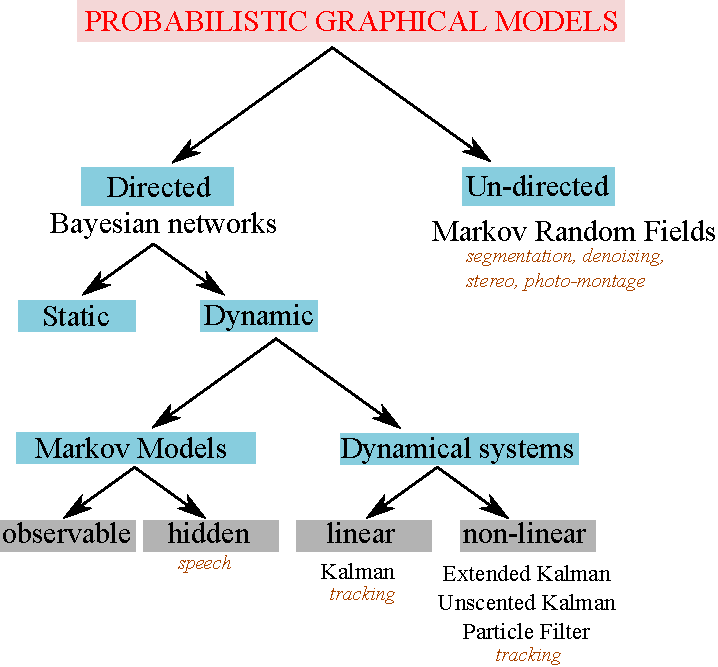
\includegraphics[width=0.7\textwidth]{figs/PRML_PGM_overview.pdf}
								\caption{Tracking, big picture.}
								\label{fig:TRK_big_picture}
								\end{figure}


\begin{itemize}
\item \underline{Assumptions related to camera}.  A common assumption, in particular in surveillance applications, is a stationary camera that allows for background maintenance.  Known camera-motion is also used although it is less common.
\item \underline{Assumptions related to target}.  These assumptions include constant velocity, constant acceleration, coherent motion (all parts of the target move together) and motion along a straight path.
\end{itemize}

								\begin{figure}[t]
								\center
								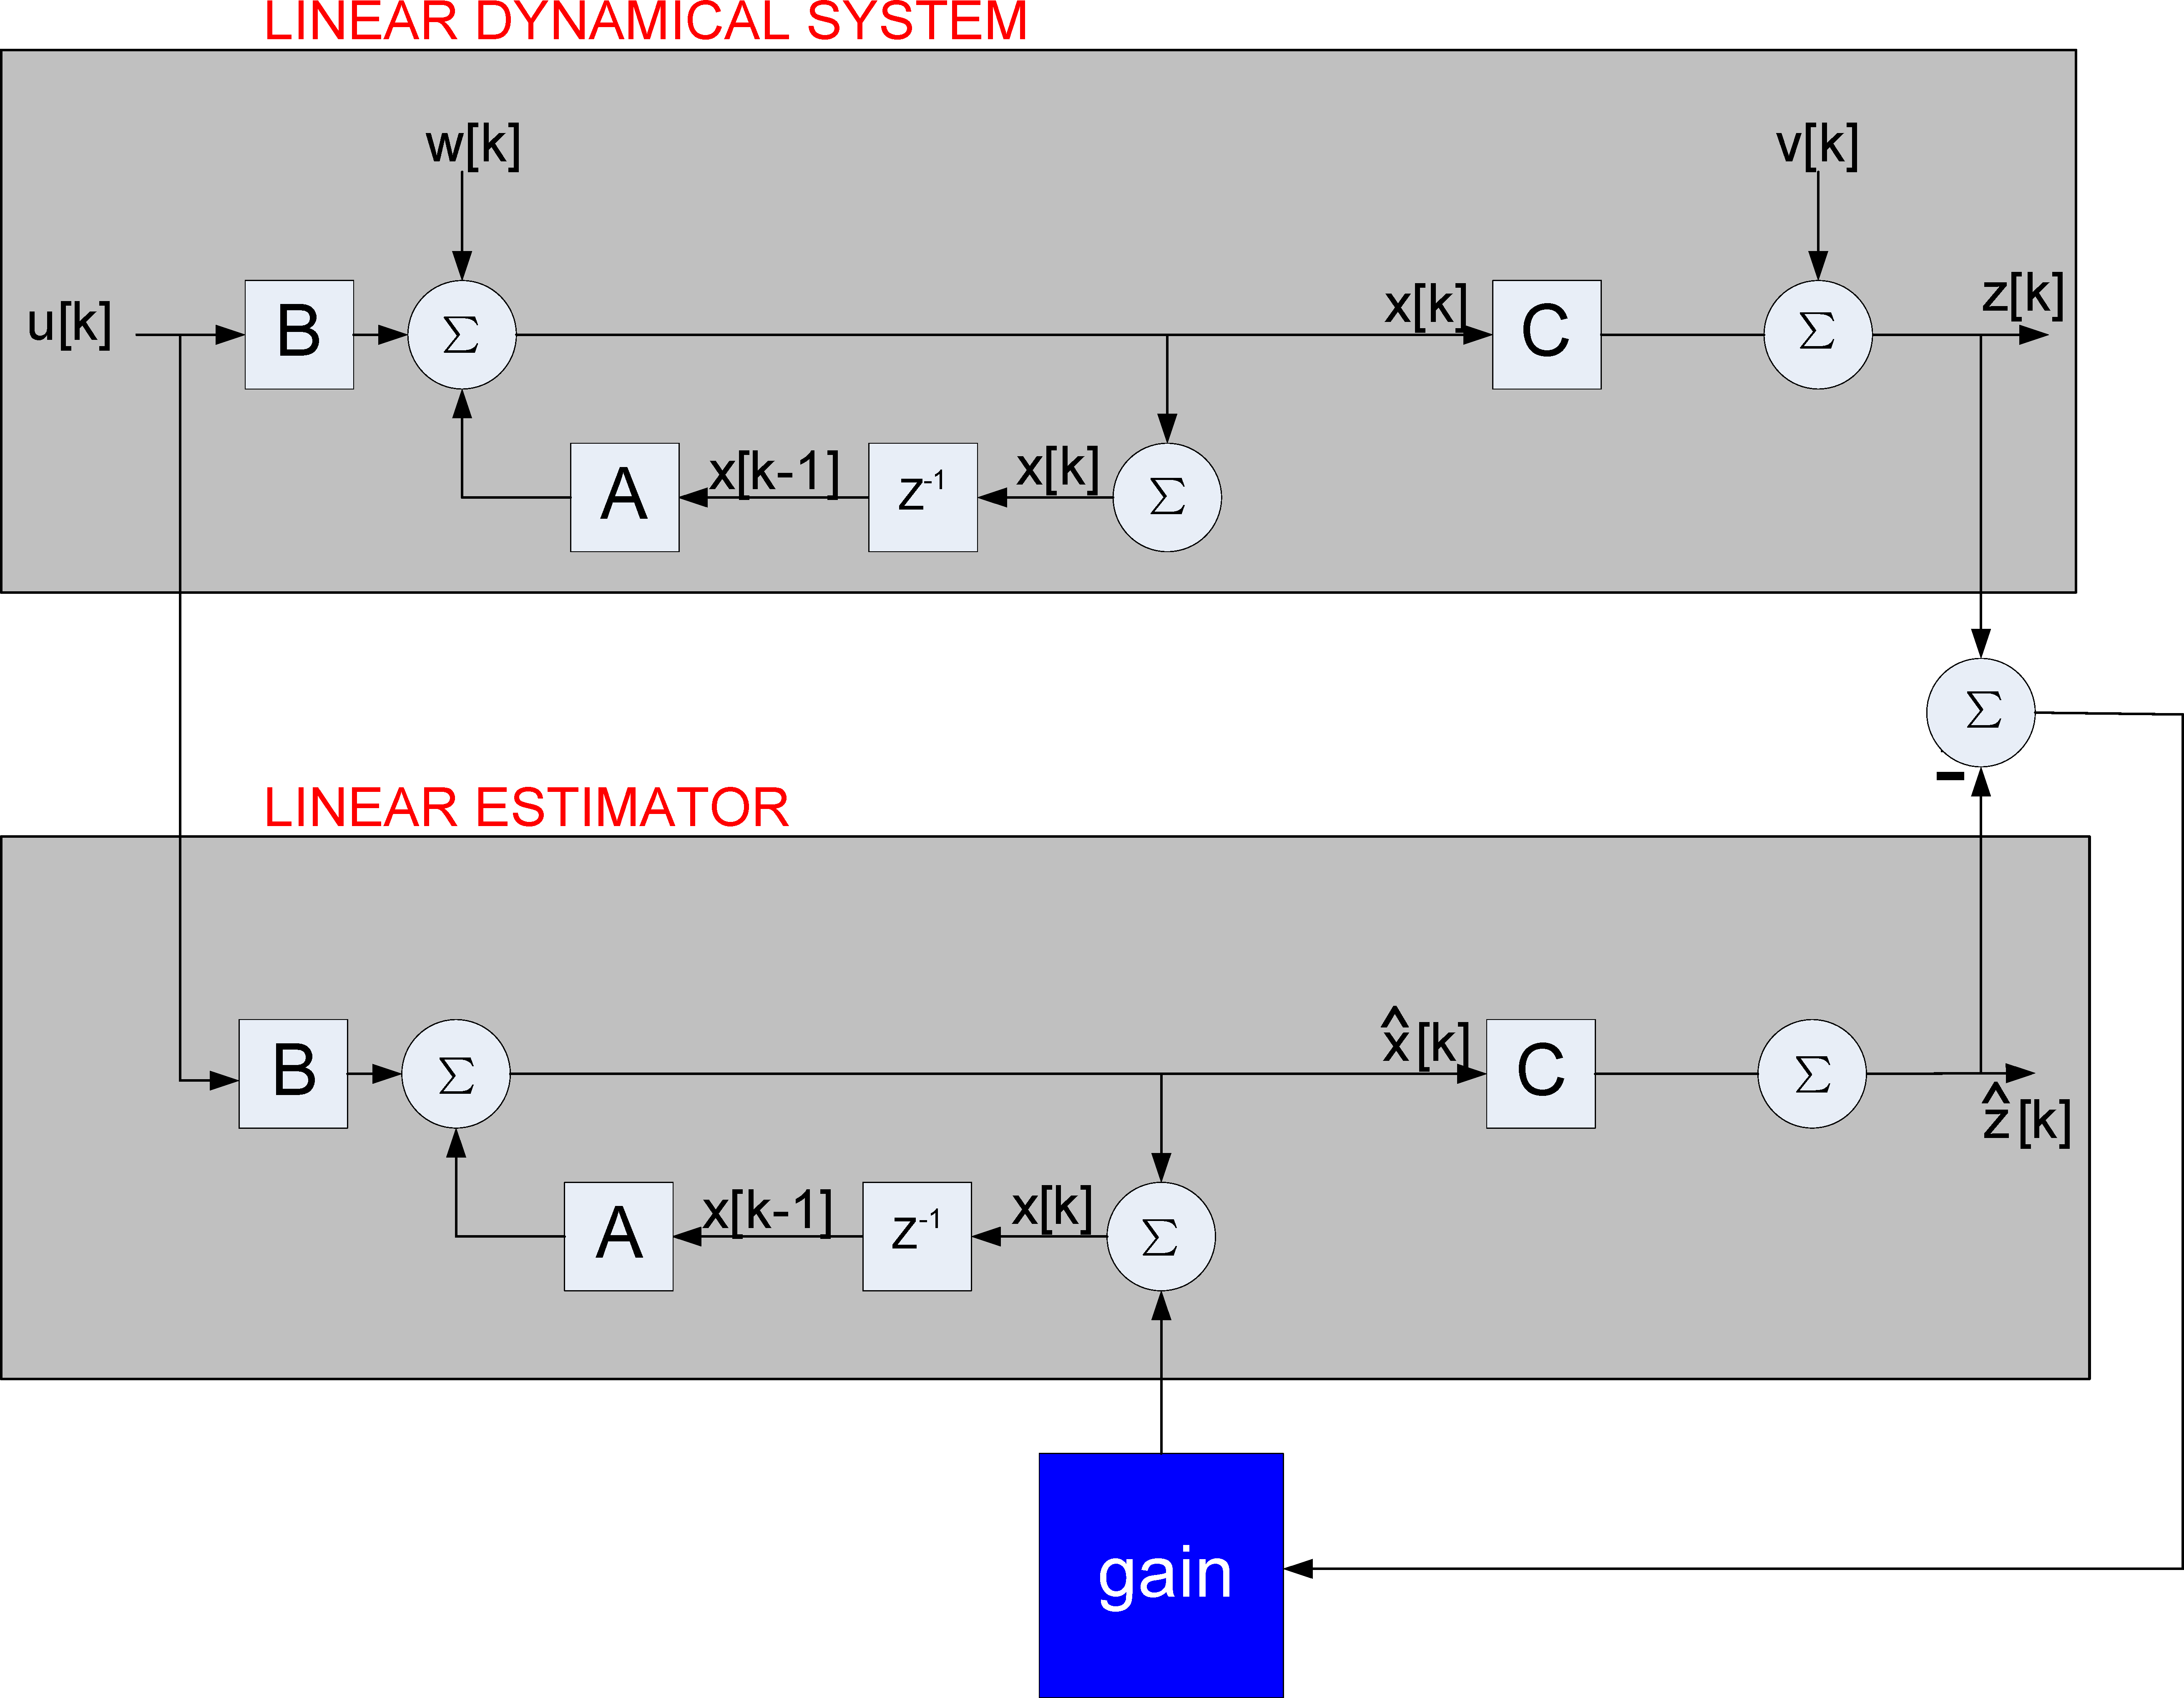
\includegraphics[width=1.0\textwidth]{figs/TRK_LinearEstimator_blockDiagram.pdf}
								\caption{Linear estimator.  The gain block is called the \emph{Kalman gain} for the Kalman filter.}
								\label{TRK_overviewDiagram}
								\end{figure}

Furthermore, several pre-processing steps may be required before tracking can be initiated.  These include stabilization for video registration, normalization, downsampling, background modeling and feature extraction.  Refer to~\cite{1999_CNF_Wallflower_Toyama} for a survey on background modeling. Commonly used features include corners, area, color, intensity distributions, contour descriptors and depth.

								\begin{figure}[t]
								\center
								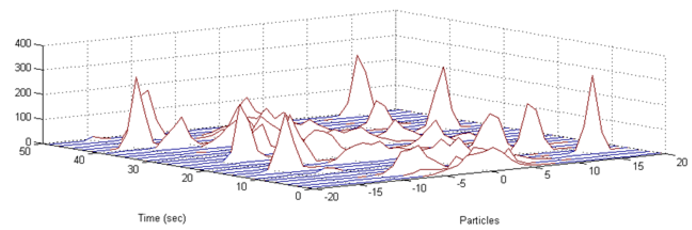
\includegraphics[width=1.0\textwidth]{figs/TRK_ParticleFilter_multimodalPDF_part.png}
								\caption{Tracking using a particle filter.  Notice that the density is non-Gaussian and multi-modal.}
								\label{fig:particle_filter_multi_modal_density}
								\end{figure}



%#######################		
\section{Bayesian estimation}
%#######################
A commonly used formulation for tracking is based on Bayesian estimation.  In this framework, target kinematics are modeled as the latent states of a time-dynamic system~\cite{2002_JNL_PF_Arulampalam}.  Time-dynamic systems are based on two models: (a) \emph{state prediction model}, ${f_t:R^D \times R^D \rightarrow R^D}$, describing state evolution, and (b) \emph{observation model}, ${h_t:R^N \times R^N \rightarrow R^N}$, relating observations to the states.  These models are described as,

\begin{align}
\mathbf{x}_t &= f_t(\mathbf{x}_{t-1}, \mathbf{v}_{t-1}) \notag\\
\mathbf{z}_t &= h_t(\mathbf{x}_t, \mathbf{n}_t)
\label{Eq:TDS}
\end{align}

$\mathbf{v} \in R^D$ is an independent, identically-distributed (IID) process noise sequence.  $\mathbf{n} \in R^N$ is an IID measurement noise sequence.  The goal is to find the estimate of the state $\mathbf{x}_t$ at time $t$, based on all observations $\mathbf{Z}_t={\{\mathbf{z}_i, i=1,...,T\}}$.   $\mathbf{z}_t$ is the observation vector at time $t$.  

At this point, it is interesting to place the process of tracking in the bigger picture of probabilistic graphical models, as shown in Figure~\ref{fig:TRK_big_picture}.  Mathematically, hidden Markov models (HMMs) can also be written using evolution and observation models even though the method was developed independently of time dynamic systems \cite{2007_BOOK_PRML_Bishop}.  

This two stage model lends itself well to Bayesian inference \cite{2002_JNL_PF_Arulampalam}.  The reason is that observations can be used as evidence to modulate the prior distribution on the states.  We can then infer the posterior distribution on the states using Bayes' Rule.  Mathematically, the Chapman Kolmogorov equation predicts the next state by combining information from the state prediction model $p(\mathbf{x}_t| \mathbf{x}_{t-1})$ and all previous observations $\mathbf{Z}_{t-1}$.  %This is given in Equation~\ref{Eqn:TRK_prediction}.

{%\Large
\begin{equation}
\begin{array}{lllllllll}
{\color{darkgreen}p(x_t|Z_{t-1})} &= \frac{p(x_t, Z_{t-1})}{p(Z_{t-1})}\\
&=\frac{\int p(x_t, x_{t-1}, Z_{t-1})dx_{t-1}}{p(Z_{t-1})}\\
&=\frac{\int {\color{Cyan}p(x_t|x_{t-1}, Z_{t-1})}p(x_{t-1},Z_{t-1})dx_{t-1}}{p(Z_{t-1})}\\
&=\frac{\int {\color{Cyan}p(x_t|x_{t-1})}{\color{red}p(x_{t-1}|Z_{t-1})}p(Z_{t-1})dx_{t-1}}{p(Z_{t-1})}\\
&=\int {\color{Cyan}p(x_t|x_{t-1})}{\color{red}p(x_{t-1}|Z_{t-1})}dx_{t-1}
\end{array}
\label{Eqn:TRK_prediction}
\end{equation}
}


%\begin{equation}
%p(x_k|\textbf{Z}_{k-1})=
%\int{p(\mathbf{x}_k| \mathbf{x}_{k-1})p(\mathbf{x}_{k-1}|\mathbf{Z}_{k-1})}d\mathbf{x}_{k-1}
%\label{eq:ChapmanKolmogorov}
%\end{equation}  

In the second step, the observation $\mathbf{z}_t$ at time $t$ and the predicted state $\mathbf{x}_t$ can be used to compute the posterior estimate of the state $\mathbf{x}_t$ using %Equation~\ref{Eqn:TRK_update}.


{%\large
\begin{equation}
\begin{array}{lllllllll}
{\color{red}p(x_t | Z_t)} &= \frac{p(x_t, Z_t)}{p(Z_t)}\\
&= \frac{p(x_t, z_t, Z_{t-1})}{p(z_t, Z_{t-1})}\\
&= \frac{{\color{blue}p(z_t|x_t,Z_{t-1})}p(x_t, Z_{t-1})}{p(z_t|Z_{t-1})p(Z_{t-1})}\\
&= \frac{{\color{blue}p(z_t|x_t)}{\color{darkgreen}p(x_t|Z_{t-1})}p(Z_{t-1})}{p(z_t|Z_{t-1})p(Z_{t-1})}\\
&= \frac{{\color{blue}p(z_t|x_t)}{\color{darkgreen}p(x_t|Z_{t-1})}}{\int{p(z_t|x_t){\color{darkgreen}p(x_t |Z_{t-1})}}dx_t}
\end{array}
\label{Eqn:TRK_update}
\end{equation}
}



%\begin{equation}
%p(\mathbf{x}_k|\textbf{Z}_k)	= \frac{p(\mathbf{z}_k|\mathbf{x}_k)p(\mathbf{x}_k |\textbf{Z}_{k-1})   }{p(\mathbf{z}_k| \textbf{Z}_{k-1})}
%\label{eq:posterior}			
%\end{equation}

Equations~\ref{Eqn:TRK_prediction} and~\ref{Eqn:TRK_update} form the optimal Bayesian solution for the recursive propagation of the posterior density.  This problem can be solved analytically using the closed-form Wiener-Kalman linear Minimum Mean Square Estimate (MMSE) in Gaussian noise \cite{1964_JNL_BayesianEstimation_Ho, 1993_BOOK_SSP_Kay}.  Non-analytical methods, such as grid-based methods, can be used if the state space is discrete and consists of a finite number of states.  For non-linear models, the Extended Kalman Filter (EKF) computes the Jacobian for a Taylor Series expansion of the system and observation models about the current state \cite{2005_Misc_KalmanFilterComparison_Orderud}.  Recently, the Unscented Kalman Filter (UKF) has been replacing the EKF in a wide range of applications.  The UKF, instead of explicitly computing the Jacobian, computes a set of points that capture the true mean and covariance of the prior.  When propagated through the non-linear system, these points capture the posterior mean and covariance \cite{1997_CNF_UKF_Julier}.  As a result, the UKF estimates the posterior mean and covariance accurately to at least the second-order Taylor Series expansion.  The EKF on the other hand achieves only first-order accuracy \cite{2004_CNF_SigmaPointKalman_Merwe, 2000_CNF_UKF_Wan}.  More recently, particle filters which use point mass representations for probability densities and are based on stochastic sampling have been introduced in the visual tracking literature \cite{1993_JNL_ParticleFilter_Gordon, 2001_JNL_PFjumpMarkov_Doucet}.  A primary difference between the UKF and the particle filter is that the former is based on deterministic sampling while the latter is based on stochastic sampling.  Particle filters offer an additional advantage of being able to handle arbitrary densities as shown in Figure~\ref{fig:particle_filter_multi_modal_density}.  However, since the particle filter uses non-parametric densities with no functional representations, its computations do not scale well as the dimensionality increases~\cite{2004_CNF_TrackingPeople_Zhao}.  

A variety of particle filters have now been introduced.   According to~\cite{2002_JNL_PF_Arulampalam}, sequential Monte Carlo (SMC) filtering has been called particle filtering~\cite{1999_CNF_PF_carpenter}, bootstrap filtering~\cite{1993_JNL_ParticleFilter_Gordon}, the condensation algorithm~\cite{1998_JNL_Condensation_IsardBlake}, interacting particle approximations~\cite{1999_JNL_PF_Crisan, 1999_BK_PF_Moral} and survival of the fittest~\cite{1995_CNF_PF_Kanazawa}.

  
%The particle filter formulation is generally similar to the method which is used for the Kalman Filter.  A prediction step is followed by an update step, which is followed by a prediction step, and so on.  The update equation at time $t$ for a state $x_t$ given all observations $z_T$ involves computing the posterior density $p(x_t | Z_t)$.  In this case, the posterior density factors into a likelihood at time $t$, $p(z_t|x_t)$ and a prior density, $p(x_t|Z_{t-1})$, 
%
%
%
%
%The prior density can be computed using the Chapman-Kolmogorov equation by introducing the nuisance parameter $x_{t-1}$,
%
%
%$p(x_t|x_{t-1})$ is computed using the motion model while $p(x_{t-1}|Z_{t-1})$ is the posterior density from the previous time step, $t-1$.
%
%
%Visual tracking in clutter is difficult using the Kalman filter since clutter can typically give rise to several competing observations which encourage a non-unimodal density and gaussian densities cannot represent simultaneous alternative hypotheses~\cite{1998_JNL_Condensation_IsardBlake}.  Moreover 


%However, currently, the most popular version is the SIR (Sampling Importance Resampling) filter \cite{2009_BOOK_PF_Doucet}.  The resampling step prevents the posterior from collapsing to a single point.  The steps involved in computing the solution to this filter are summarized below:

%\begin{itemize}
%\item \textbf{Sampling with replacement.}  This step is carried out to guarantee that the algorithm runs within given computational resources.  $N$ samples are chosen from the set $\mathbf{s}_{k-1}^n$, each element being chosen with probability $\pi_{k-1}^n$.  %a sampling with replacement st from $p(\mathbf{x}_k | \mathbf{x}_{k-1})$
%\item Calculate particle weights from the likelihood, $\mathbf{w}_k = p(\mathbf{z}_k|\mathbf{x}_k)$
%\item Calculate the posterior ($p(\mathbf{x}_k | \mathbf{x}_{k-1})$.  First normalize weights.  Then resample using normalized-weights and sampled-prior. 
%\end{itemize}









%#######################		
\section{Traditional methods}
%#######################


\subsection{Point tracking}
%==========================
The problem of point tracking in the field of Computer Vision is similar to the problem of point tracking in the field of Radar Signal Processing.  This problem has been extensively studied and is also known as the \emph{data association} problem.  In Computer Vision, an additional pre-processing step, \emph{interest-point detection}, is required to extract points of interest from the scene.  Point tracking methods can be broadly categorized into statistical methods and deterministic methods.

There are three main statistical methods for point tracking.  The \emph{Probability Data Association Filter (PDAF)} provides a computationally efficient method of data association for single targets \cite{1975_JNL_PDAF_BarShalom}.  It is largely based on the Kalman Filter.  However, it has a mechanism of accounting for clutter.  The primary difference between the Kalman filter and the PDAF algorithm is in the computation of the innovations process during the update stage.  For multiple targets, this algorithm is generalized by the \emph{Joint Probability Data Association Filter (JPDAF)}~\cite{1983_JNL_JPDAF_Fortmann}.  The \emph{Multiple Hypothesis Tracker (MHT)} handles multiple targets in non-linear conditions~\cite{1979_JNL_MTT_Reid}.  MHT requires ever-expanding memory as more and more data is processed.  However, computationally practical versions of MHT have been reported \cite{1996_JNL_EfficientMHT_Cox, 1994_CNF_MLPMHT_Streit}.  It may be noted that a carefully designed MHT can provide better performance than the PDAF and JPDAF algorithms \cite{2009_JNL_PDAF_Barshalom}.  Additional details can be found in a survey by Cox \cite{1993_JNL_SURVEYcorresp_Cox}.  

Statistical methods have a number of shortcomings.  First, the assumption that points move independently is not always valid.  Second, measurements are not always distributed normally around their predicted position.  Third, there are a number of parameters to estimate, such as apriori probabilities for false measurements and missed detections.  And finally, statistical methods can be computationally demanding \cite{2001_JNL_MotionCorrespondence_Veenman}.  To deal with these shortcomings, a number of researchers have worked on deterministic methods for point tracking.

Most deterministic methods minimize a cost of associating a target to an observation.  This correspondence cost is usually a combination of several constraints \cite{2006_JNL_SURVEYtrk_Yilmaz}: (a) proximity, (b) maximum velocity, (c) smooth motion, (d) common motion, and (e) rigidity.  A \emph{zero-scan} algorithm uses one frame for correspondence and picks the maximum likelihood hypothesis at every time frame.  On the other hand, a \emph{multiple-scan} algorithm uses multiple frames for correspondence \cite{1979_JNL_MTT_Reid}.    Sethi and Jain \cite{1987_JNL_FeatureTrajectories_Sethi} use path coherence and motion smoothness for solving the correspondence problem.  Unlike many previous approaches, they solve the correspondence problem using multiple frames rather than two.  Salari and Sethi \cite{1990_JNL_PointCorresp_Salari} extend this work to handle occlusions.  Rangarajan and Shah \cite{1991_JNL_MotionCorrespondence_Rangarajan} use a greedy non-iterative algorithm with a fixed number of feature points while allowing for temporary occlusion and missing point detections.  A \emph{common-motion} constraint is introduced in \cite{2001_JNL_MotionCorrespondence_Veenman}.  According to this constraint, two points lying on the same object should move coherently.  Finally, a generic and widely used one-to-one correspondence algorithm is the Hungarian algorithm \cite{1955_JNL_HungarianMethod_Kuhn}.

\subsection{Region tracking}
%==================================================
Several methods for tracking regions have been proposed in the literature.  We describe some of the more popular methods in the next few paragraphs.

\emph{Template matching} is one of the most common methods for tracking regions.  This method involves matching the sub-region of an image with a template.  A variety of distance measures have been used in template matching.  Some commonly used distance measures are SSD (sum of squared differences), SAD (sum of absolute differences) and correlation (CORR).  These measures can be computed using the following equations:


\begin{align}
SSD(x,y)  &=\sum_{x'}\sum_{y'} {[I(x+x', y+y')-t(x', y')]}^2 \notag\\
SAD(x,y)  &=\sum_{x'}\sum_{y'} |I(x+x', y+y')-t(x', y')| \\
CORR(x,y) &=\sum_{x'}\sum_{y'} I(x+x', y+y') t(x', y') \notag
\end{align}

SAD is widely used in the video coding literature.  As a matter of fact, it is used in almost all current video codecs, i.e., MPEG-1, MPEG-2, MPEG-4, H.261, H.263, and H.264.  The method of template matching has been applied in many areas of Computer Vision, including tracking.  Some examples of the usage of template matching are head tracking \cite{1998_CNF_HeadTracking_Birchfield}, motion identification \cite{1998_CNF_Tracking_Lipton, 2001_JNL_MotionTemplates_Bobick}, contour matching \cite{2009_CNF_HumanDetection_Beleznai}, human detection \cite{2010_JNL_HumanDetectionSegmentation_Lin}, pedestrian detection \cite{1997_CNF_PedestrianDetection_Oren}, finger tracking \cite{1995_CNF_Tracking_Rehg}, object recognition \cite{2000_CNF_MLtemplateMatching_Olson} and track initialization \cite{1998_CNF_Tracking_Lipton, 2010_CNF_TrkRVQ_Aslam}.  The advantages of template matching are simple implementation and robustness to short-term, gradual changes in appearance.  The disadvantages of template matching are high computational cost, failure under occlusions, and the need for updating over time.  However, methods exist to overcome some of these shortcomings.  Fast template matching \cite{2002_CNF_FastTemplateMatching_SchweitzerBellWu} and template updating are some of the solutions \cite{1998_CNF_Tracking_Lipton} proposed in the literature.

A number of researchers have used density based methods to track regions.  The Bhattacharya coefficient $\rho$ for two densities $p_i(x)$, and an associated distance measure, the Bhattacharya distance $B$ \cite{1967_JNL_Bhattacharyya_Kailath} have been commonly used to compare densities.  $\rho$ and $B$ are given by 

\begin{align}
\rho &= \int p_1(x)p_2(x) \notag\\
B &= -\text{ln}(\rho)
\label{Eq:Bhattacharya}
\end{align}

A commonly used method of density tracking is the \emph{mean-shift} algorithm.  In this algorithm, the gradient vector of the density is computed.  Repeated iterations lead to a local mode of the density.  This algorithm starts with a Parzen non-parametric density for $n$ data points, $x_i$, $i=1..n$, in $d$-dimensional space $R^d$.  This density is given by \cite{2007_BOOK_PRML_Bishop},

\begin{equation}
f(\mathbf{x}) = \frac{1}{nh^D}\sum_i K(\frac{\mathbf{x}-\mathbf{x}_i}{h})
\label{Eq:ParzenDensity}
\end{equation} 

where $h^D$ is the volume of a hypercube of side $h$ in $R^d$.  The gradient of this density is given by

\begin{equation}
\nabla f(\mathbf{x}) = \frac{2c}{nh^{D+2}} 
\left[ \sum_{i=1}^n  g \left({ \left\|   \frac{\mathbf{x}-\mathbf{x}_i}{h}\right\| }^2 \right) \right] 
\left[ \frac{ \sum_{i=1}^n  \mathbf{\mathbf{x}_i}g \left({ \left\|   \frac{\mathbf{x}-\mathbf{x}_i}{h}\right\| }^2 \right)}{\sum_{i=1}^n  g \left({ \left\|   \frac{\mathbf{x}-\mathbf{x}_i}{h}\right\| }^2 \right)} -\mathbf{x}\right] 
\end{equation}

where $c$ is a constant, $\left[ \sum_{i=1}^n  g \left({ \left\|   \frac{\mathbf{x}-\mathbf{x}_i}{h}\right\| }^2 \right) \right]$ is proportional to the density estimate at \textbf{x}, and $\left[ \frac{ \sum_{i=1}^n  \mathbf{\mathbf{x}_i}g \left({ \left\|   \frac{\mathbf{x}-\mathbf{x}_i}{h}\right\| }^2 \right)}{\sum_{i=1}^n  g \left({ \left\|   \frac{\mathbf{x}-\mathbf{x}_i}{h}\right\| }^2 \right)} -\mathbf{x}\right]$ is the \emph{mean-shift}.  The mean-shift always points in the direction of the density gradient, i.e., direction of maximum increase of the density.  Repeated application of this formula results in a series of mean-shift vectors which define a path leading to a stationary point of the estimated density \cite{2002_JNL_MeanShift_Comaniciu}.  This method has been successfully used in a number of scenarios including human tracking in dense crowds \cite{2000_CNF_RealTimeTrackingMeanShift_Comaniciu}, compressed video tracking \cite{2009_CNF_Compensation_Aslam} and airborne tracking in infra-red images \cite{2003_JNL_AirborneIRtracking_Yilmaz}.  

Finally, \emph{optical flow} is a method of computing the motion between two successive frames.  Since motion computation is an ill-posed problem, two constraints are commonly used to compute a solution: (a) brightness constraint, i.e. $I(x,y,t) = I(x+\delta x,y+\delta y,t+\delta t)$ and, (b) smooth velocity constraint, i.e. $\nabla^2 u + \nabla^2 v$, where $I(x,y,t)$ is an image pixel in image $I$ at location $(x,y)$ at time $t$, $u=dx/dt$ is the velocity in the x-direction, and $v=dy/dt$ is the velocity in the y-direction.  An iterative scheme to compute optical flow is given by Horn and Schunk \cite{1981_JNL_OpticalFlow_HornSchunck}.  An alternate method is given by Lucas and Kanade \cite{1981_CNF_IterativeImageRegistration_LucasKanade}.  A comparison of optical flow techniques can be found in \cite{1994_JNL_PerfOpticalFlow_Barron}.  Motion information is a useful feature in tracking.  However, in many tracking scenarios, optical flow assumptions of brightness constancy do not hold.  This is particularly true when multiple targets are being tracked and occlusions are common.  Nevertheless, some attempts at robust tracking have been made in these difficult situations \cite{1996_CNF_MultipleMotionsFlowFields_Black}.

\subsection{Contour tracking}
%============================
The third and final tracking method we discuss is contour tracking.  We describe some of the methods in this category in the next few paragraphs.

A closed contour can be represented by an Elliptical Fourier decomposition \cite{1982_JNL_EllipticalFourier_Kuhl} given by

\begin{align}
\centering
	\label{eq:EllipticalFourierTransform}
	a_0&=\frac{1}{2\pi}\int_0^{2 \pi}x(t)dt,       \notag\\ 
	c_0&=\frac{1}{2\pi}\int_0^{2 \pi}y(t)dt,       \notag\\ 
	a_k&=\frac{1}{\pi}\int_0^{2 \pi}x(t)cos(kt)dt,   \ \ \   b_k=\frac{1}{\pi}\int_0^{2 \pi}x(t)sin(kt)dt    \notag\\
	c_k&=\frac{1}{\pi}\int_0^{2 \pi}y(t)cos(kt)dt,    \ \ \  d_k=\frac{1}{\pi}\int_0^{2 \pi}y(t)sin(kt)dt    \notag\\
	\left[ \begin{array}{ccc}x(t) \\y(t) \end{array}\right] &=\left[ \begin{array}{ccc}a_0\\c_0 \end{array}\right] + \sum_{k=1}^K \left[ \begin{array}{ccc}a_k & b_k\\c_k & d_k \end{array}\right]\left[ \begin{array}{ccc}cos(kt)\\sin(kt) \end{array}\right]
\end{align}

This method has been used for contour tracking in infra-red images \cite{2010_CNF_VehicleContour_Aslam}.  However, this method has not been widely used for tracking.  We mention this technique for the sake of completeness, and to compare it to other contour based methods.  One of the reasons that this method has not been widely adopted for tracking is that it is difficult to incorporate prior information in the parameterization of Equation \ref{eq:EllipticalFourierTransform}.  The next few techniques address this issue.

The \emph{snakes} method \cite{1988_JNL_Snakes_Kass} is a contour evolution method.  In this method, a spline curve is represented parametrically as $\mathbf{v}(s) = (x(s), y(s))$.  Its energy functional is given by

\begin{align}
E_{snake} &= \int_0^1 E_{snake}(\mathbf{v}(s)) \notag\\
&=\int_0^1 E_{int}(\mathbf{v}(s)) + E_{ext}(\mathbf{v}(s)) ds
\label{Eq:Snakes}
\end{align}

where $E_{int}$ is the internal energy of the spline, and can be written as a sum of two terms: (a) membrane energy ($\frac{\alpha}{2}(x_s^2 + y_s^2)$), and (b) thin-plate energy ($\frac{\beta}{2}(x_{ss}^2 + y_{ss}^2)$).  $E_{ext}$ is the external energy and is derived from the image.  This additional term makes it possible to incorporate prior information about the image.  This is in contrast to Elliptical Fourier Descriptors.  A commonly used external energy term is the gradient evaluated along the contour.  In this case, Equation \ref{Eq:Snakes} can be written as

\begin{equation}
	\label{eq:SnakesEnergy1}
	E=\int_0^1 \left[\frac{\alpha}{2}(x_s^2 + y_s^2) + \frac{\beta}{2}(x_{ss}^2 + y_{ss}^2) - \left[\nabla{(x(s), y(s))}\right]\right]dt
\end{equation}

In order to model more complex shapes, level-sets were introduced in \cite{1995_JNL_LevelSets_Malladi}.  In this formulation, a contour is represented as the zero crossings in a level-set grid.  The evolution of the contour is governed by changing the grid values \cite{2006_JNL_SURVEYtrk_Yilmaz}.  Snakes have been used in a variety of applications, including walker tracking \cite{1994_CNF_WalkingFiguresXYT_Niyogi}, head tracking \cite{2001_JNL_ProbabilisticDataAssociation_Rasmussen}, and vehicle and hand tracking \cite{1999_JNL_KalmanSnakes_Peterfreund}.

A further extension to the snakes model is the \emph{active-appearance model}, or "smart" snake model, proposed by Cootes et al. \cite{1995_JNL_ActiveModels_Cootes}.  In this approach, structural constraints derived from a training set are imposed on the model.  This is done to guide the shape evolution.  As a result, this method captures the natural variability within a class of shapes.  The advantage over snakes is that shape deformation is always consistent with the training set.  This method has also been applied to tracking.  Examples include human tracking \cite{1994_CNF_ContourTracking_BaumbergHogg, 2003_JNL_ActiveShapeTracking_Koschan}.


\subsection{Complete trackers}
%=================
The tracking techniques mentioned in the last three sections, i.e. point tracking, region tracking and contour tracking, have been applied to a variety of applications.  In particular, a lot of attention has been given to human tracking.  In the following few paragraphs, we summarize the major research in this important area.


\begin{itemize}
\item \underline{KidsRoom \cite{1997_CNF_ClosedWorldTracking_Intille}}:  This system tracks little children in a reasonably realistic environment.  A background model is used to generate blobs.  Four features are used for tracking: average normalized color, distance, velocity and size.  

\item \underline{Pfinder \cite{1997_JNL_Pfinder_Wren}}.  This work popularized background subtraction \cite{2006_JNL_SURVEYtrk_Yilmaz}.  The advantage of background subtraction is that it can lead to a blob based representation.  Such a representation reduces the degrees of freedom in going from individual pixels to blobs.  In this sense, it is a form of regularization.  The Pfinder system tracks a single user.  The features used for tracking include skin color and 2D shape contour for head, hands and feet.  For each pixel, a likelihood is computed for each of the blob models.  The class membership likelihoods are resolved using spatial and connectivity constraints.  A major drawback of this system is the process of initialization in which a user is required to carry out specific actions.

\item \underline{CMU \cite{1998_CNF_Tracking_Lipton}}.  This is a classification and tracking system.  This system is based on the fact that properties of template matching and temporal differencing (DT) are complementary.  When the target is stationary, template matching is at its most robust, while DT does not do well.  If the target is moving, template matching does not do well while DT does.  This system classifies and tracks humans and cars based on size and \emph{dispersedness} ($\frac{{perimeter}^2}{area}$).  MLE is used for classification.  The templates are updated using an IIR filter.

\item \underline{W4 \cite{2000_JNL_W4_Haritaoglu}}:  This system detects foreground objects using a background, bimodal-gaussian, intensity distribution.  No use of color is made.  In comparison, Pfinder uses color information.  Another difference is that unlike Pfinder, W4 does not assume that there is only one person in the scene.  The features used are shape and appearance models.  Besides tracking humans, this system can recognize simple events such as carrying, leaving or exchanging bags.

\item \underline{Bramble \cite{2001_CNF_TRKhuman_Isard}}.  This system uses a known camera model and ground plane.  It can therefore track humans in 3D.  The state estimation is done using particle filters.  

\item \underline{Zhao and Nevatia \cite{2004_CNF_TrackingPeople_Zhao}}.  This state-of-the-art tracker simultaneously tracks up to 13 people in a crowd.  The researchers use a color-histogram based mean-shift tracker for appearance model correspondence.  The human body is modeled using a 3-ellipsoid, one for the head, one for the torso, and one for the legs.  The prior has spatial and temporal components.  The spatial prior penalizes unnecessary overlapping of targets and blobs with small sizes.  The temporal prior encourages smoothness and trajectory connectivity.  The likelihood is computed using background exclusion and correspondences.  The MAP estimate is computed using MCMC sampling.  State estimation for velocity is done using the Kalman filter.

\item \underline{Brostow and Cipolla \cite{2006_CNF_TRKhuman_Brostow}}  This tracker is also state-of-the-art.  An unsupervised Bayesian clustering method is used to detect individuals moving in crowded scenarios.  Interestingly, the only feature used is motion.  No training data is used, nor is there any appearance model.  The idea is to probabilistically cluster regions moving in unison.  Motion initialization is done using optical flow.  Subsequently, normalized cross correlation is used to match corners.  Regions with similar motion are clustered to form targets.
\end{itemize}

%#######################		
\section{Subspace based tracking}
%#######################
An adaptive subspace representation has several advantages:

\begin{itemize}
\item \textbf{Compact representation}.  A subspace represenation using say PCA or RVQ allows storage of a few basis eigenvectors or stage codevectors to capture variations in the target appearance.
\item \textbf{Object recognition}.  This method facilitates object recognition since an appearance model is built for each target.
\item \textbf{Continuous model update}.  As mentioned earlier, changes in target appearance are a big challenge in target tracking.  Online model updating allows the target appearance to be built dynamically.
\item \textbf{Less offline training data required}.  In many instances, few training examples are available that have the same distribution as the expected tracking scenario.  Systems that rely on offline training ignore the information available during online tracking.  An adaptive subspace representation can be used effectively in these scenarios since models are built and maintained online.
\item \textbf{No optimization}.  No complex optimization is required.
\item \textbf{Camera motion}.  This representation does not depend on background maintenance and can therefore be used with moving cameras.
\end{itemize}


One of the main factors limiting visual tracking is the lack of suitable appearance models~\cite{2003_JNL_TRKsubspace_Jepson}.  A solution to this problem is to use view-based representations of objects.  The view-based approach can be interpreted to mean one of three approaches:

\begin{itemize}
\item \underline{Multi-camera approach.}  As the name suggests, several cameras are used to generate simultaneous views of an object from different angles \cite{2000_JNL_EasyLiv_Krumm}.  
\item \underline{VBR approach (training phase).}  In this approach, a limited number of views of an object are sampled as it is rotated about the x, y and z axes of rotation during a training phase.  This approach forms the basis of view-based recognition (VBR) and allows replacing the matching of a single 3D model with matching a large number of 2D models~\cite{1992_JNL_VBR_Breuel, 1993_CNF_Gestures_Darrell}.
\item \underline{Online appearance approach (testing phase).}  In this approach, several views of an object are captured as it is tracked online and used to model the dynamic appearnce of the object~\cite{2008_JNL_subspaceTRK_Ross}.
\end{itemize}
								\begin{figure}[t]
								\center
								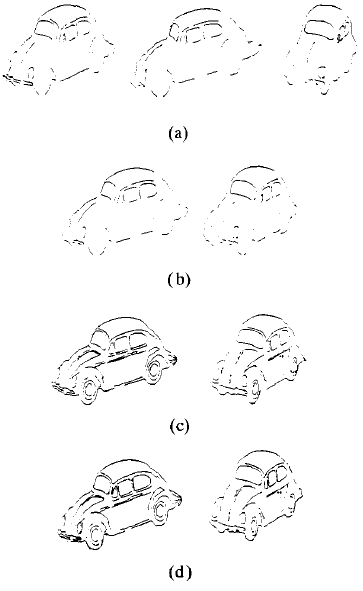
\includegraphics[height=0.6\textheight]{figs/1991_JNL_TRKsub_Ullman_fig3.png}
								\caption{(a) Original images, (b) Synthetic images created from linear combinations of original images, (c) More original images at approximately same orientation as the synthetic images, (d) Synthetic images superimposed on original images~\cite{1991_JNL_Recog_Ullman}}.
								\label{fig:1991_JNL_TRKsub_Ullman_fig3}
								\end{figure}

In this work, we do not focus on the multi-camera approach.  We start our discussion with the VBR approach and transition to the online appearance approach for two reasons: (a) it historically predates the online appearance approach, and (b) it naturally leads to the online appearance approach.

In order to classify or recognize complex articulated objects, a large range of appearances are required.  One approach has been to use interpolation of appearance from a small number of views.  \cite{1991_JNL_Recog_Ullman} makes the assumption that all possible views of an object after 3D transformations such as rotation, translation and scaling can be expressed as the linear combination of other views of the same object.  Therefore, object matching is done by finding the distance between the linear subspace (or low dimensional manifold) defined by previous views and an observed object, rather than measuring the distance between the object and each of the stored views.  Figure~\ref{fig:1991_JNL_TRKsub_Ullman_fig3} shows an example of generating different car views using linear combinations of existing views.  



								\begin{figure}[t]
								\center
								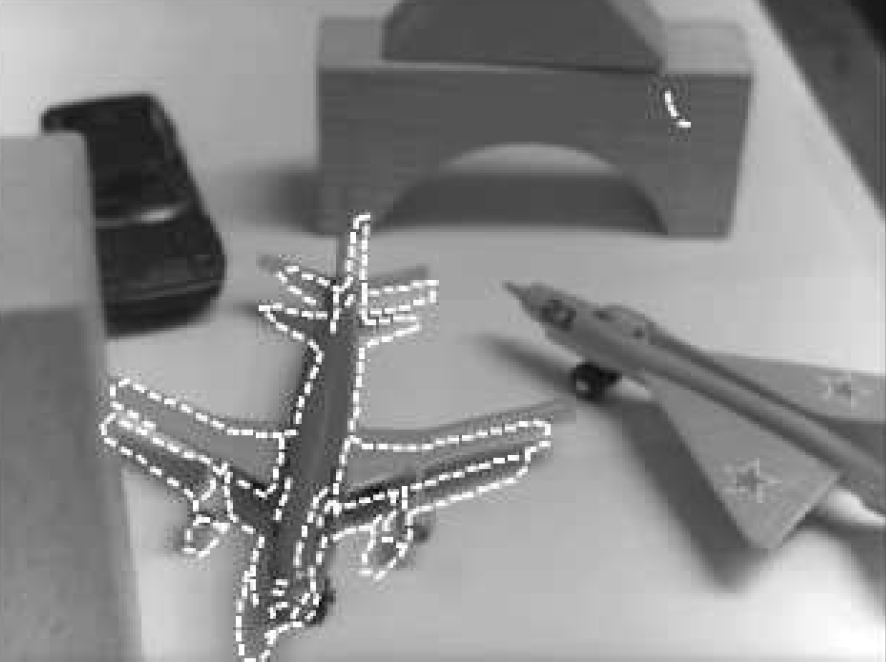
\includegraphics[width=0.6\textwidth]{figs/1992_JNL_VBR_Breuel_fig1.png}
								\caption{Airplane recognized by view-based recognition system \cite{1992_JNL_VBR_Breuel}}
								\label{fig:1992_JNL_VBR_Breuel_fig1}
								\end{figure}

A generalization to this approach points out that exact representations do not always exist for continuous functions in terms of simpler functions~\cite{1990_JNL_Network_Poggio}.  However, good and general approximating representations may exist.  For instance, interpolation can be used for hypersurface reconstruction.  Since this problem is ill-posed, i.e. generally there's not enough data for a unique reconstruction, various assumptions such as smoothness are made.  These forms of regularization can be justifed using Bayesian MAP estimation.  A theoretical framework is then developed based on regularization techniques to create a three-layer network called a \emph{regularization network} which is useful for approximation, such as interpolation.

A step forward in the justification of view-based representations is presented in  \cite{1992_JNL_VBR_Breuel}, where it is shown that 300 views need to be stored for each view-based model to achieve an error rate smaller than that of optimal 3D matching algorithms.  An example of such a matching is shown in Figure~\ref{fig:1992_JNL_VBR_Breuel_fig1}.%In these experiments, 1000 images of bent paper clips were used, each paper clip being represented by 20 line segments.  The system developed was then used to recognize real world 3D objects from several Canny edge detection generated 2D views.

A fundamental question here is how to learn an appropriate set of view models.  As mentioned earlier, in traditional tracking approaches, such as normalized correlation or template matching, there is a limitation that the image motion must be simple, such as translation and the viewpoint must be fixed or changing slowly.  \cite{1993_CNF_Gestures_Darrell} tackle this challenge by using sets of view models, rather than simple templates.  In this approach, a data-driven method of using normalized correlation scores to automatically construct a set of view models is developed.  One initial model is specified by the user using a cursor.  The target object is tracked using normalized correlation.  The search function correlation scores are saved so that when they fall below a certain threshold, a new model can be added to the search set using the image at the offset with the best current score.  Over time, a family of view models that sample the aspect space are accumulated.  Two thresholds are maintained, one for deciding if track has been lost, and the other sets the level at which a new model should be added.  This method is then used to recognize human gestures.

								\begin{figure}[t]
								\center
								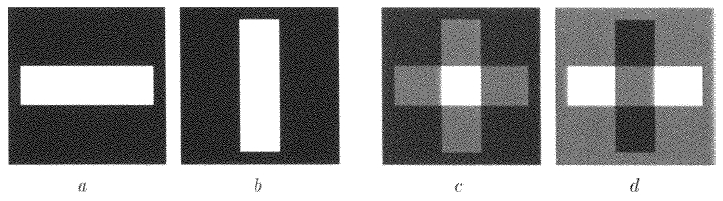
\includegraphics[width=1.0\textwidth]{figs/TrackingPapers_SubspaceTracking_1998_Black_fig2_nocaption.png}
								\caption{(a, b) Training images (c, d) Eigenspace basis images \cite{1998_JNL_Eigentracking_Black}}
								\end{figure}


								\begin{figure}
								\center
								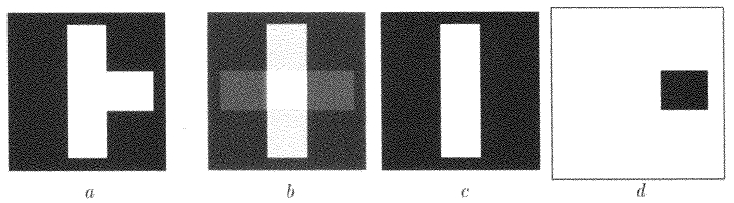
\includegraphics[width=1.0\textwidth]{figs/TrackingPapers_SubspaceTracking_1998_Black_fig3_nocaption.png}
								\caption{(a) Test image (b) Least squares reconstruction (c) Robust reconstruction \cite{1998_JNL_Eigentracking_Black}}
								\end{figure}

A multi-view method that deals with illumination changes, to which SSD (sum of squared differences) or correlation based tracking is sensitive to, is presented in \cite{1996_TRK_region_Hager}.  A set of 5 basis images is created offline for a single face under a single view but different illumination conditions.  Images with maximum singular values in the SVD decomposition are retained for the basis.  These basis images are then used to approximate the object under any illumination condition.  This work also accounts for geometric changes in the face through affine warping.  

The transition of VBR to view-based tracking is first made in the seminal work of \emph{eigentracking} presented in \cite{1998_JNL_Eigentracking_Black}.  This is an adoption of initial work in the area of PCA based methods to efficiently represent several views \cite{1995_JNL_ActiveModels_Cootes, 1991_CNF_Eigenfaces_Turk}.  Before this work, eigenspace representations had focused on the problem of object recognition and had only peripherally addressed the problem of object tracking over time.  Additionally, it was assumed that the object of interest could be located in the image, segmented and transformed into canonical form for matching with the eigenspace.  However, this is not always possible and eigenspace reconstruction methods are not invariant to image transformations such as translation, scaling and rotation.  Two primary observations are made in this work that have formed the basis of current subspace tracking methods:

								\begin{figure}[t]
								\center
								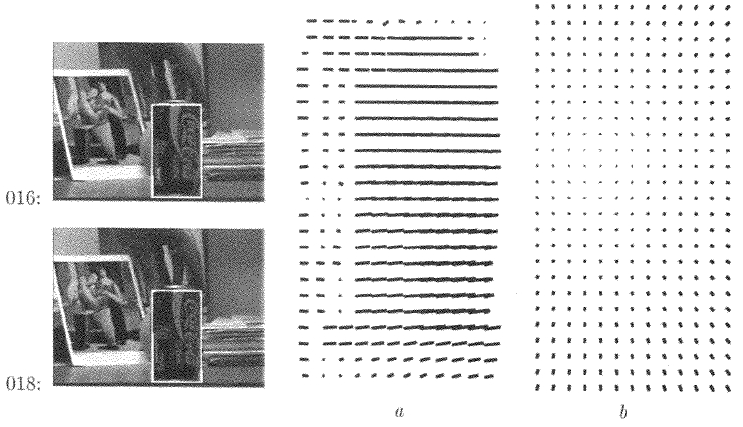
\includegraphics[width=1.0\textwidth]{figs/TrackingPapers_SubspaceTracking_1998_Black_fig11_nocaption.png}
								\caption{Brightness versus subspace constancy.  "Motion" between frames 16 and 18 ( computed within the white boxed region) (a) dense optical flow for the soda can computed using the brightness constancy assumption (b) "Flow" computed using the subspace constancy assumption for the same frames \cite{1998_JNL_Eigentracking_Black}}
								\end{figure}


\begin{figure}[t]
\centering	
\subfigure[Training image.]{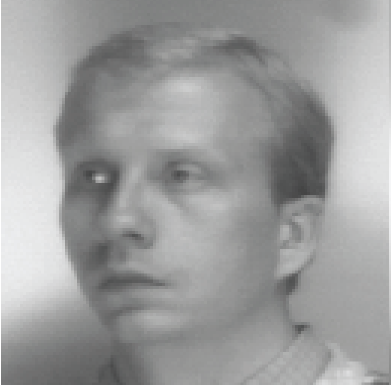
\includegraphics[width=0.3\textwidth]{figs/TrackingPapers_SubspaceTracking_1997_Moghaddam_fig13_trginp.png}}
\subfigure[Training image reconstruction, parametric eigenspace]{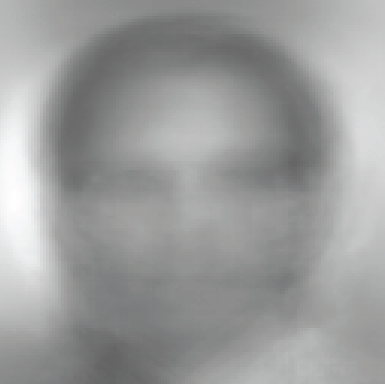
\includegraphics[width=0.3\textwidth]{figs/TrackingPapers_SubspaceTracking_1997_Moghaddam_fig13_trgout_paramPCA.png}}	
\subfigure[Training image reconstruction, view-based eigenspace]{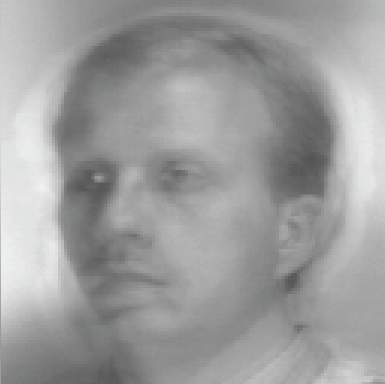
\includegraphics[width=0.3\textwidth]{figs/TrackingPapers_SubspaceTracking_1997_Moghaddam_fig13_trgout_viewPCA.png}}	
\subfigure[Test image.]{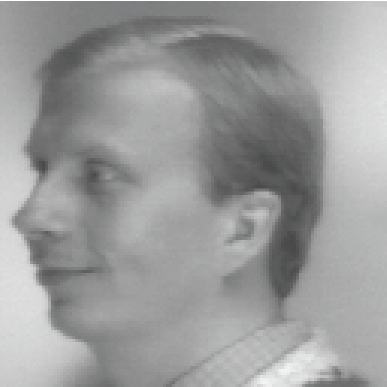
\includegraphics[width=0.3\textwidth]{figs/TrackingPapers_SubspaceTracking_1997_Moghaddam_fig13_tstinp}}	
\subfigure[Test image reconstruction, parametric eigenspace]{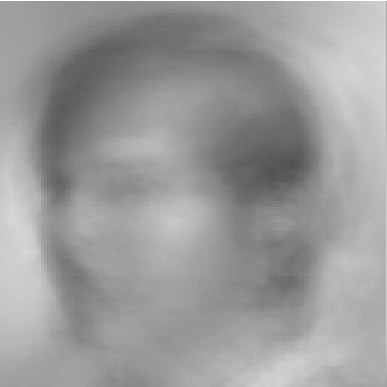
\includegraphics[width=0.3\textwidth]{figs/TrackingPapers_SubspaceTracking_1997_Moghaddam_fig13_tstout_paramPCA.png}}	
\subfigure[Test image reconstruction, view-based eigenspace]{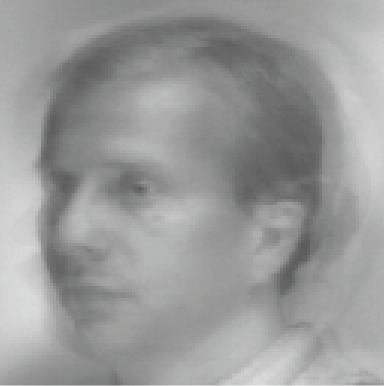
\includegraphics[width=0.3\textwidth]{figs/TrackingPapers_SubspaceTracking_1997_Moghaddam_fig13_tstout_viewPCA.png}}	
\caption{Comparing parametric eigenspace with view-based eigenspace.}								
\label{fig:parametric_vs_viewBased_eigenspace}				
\end{figure}

\begin{enumerate}
\item \underline{Robust estimation.}  PCA reconstruction relies on a least squares fit between an image and the eigenspace.  This can lead to poor results in the presence of structured noise.  This work reformulates the eigenspace matching problem as one of robust estimation.
\item \underline{Affine transformation.} Instead of storing all views of the object to be tracked or learn interpolating surfaces in the eigenspace, an affine transformation is allowed between the input image and the subspace.
\end{enumerate}

A fundamental issue of whether to create one eigenspace for all classes or one eigenspace per class is addressed in~\cite{1997_JNL_EigenTRK_Moghaddam}.  The classes correspond to $M$ human head orientations with $N$ examples in every class.  In a \emph{parametric} eigenspace, one eigenspace is created for all $NM$ images.  On the other hand, in a \emph{view-based} eigenspace, one eigenspace is created for each of $M$ head orientations, each with $N$ users per eigenspace.  Since multiple views of a face form a connected non-convex region \cite{1994_JNL_FaceTop_Bichsel}, the analogy of using a parametric versus a view-based eigenspace approach is that of modeling a complex distribution by a single cluster model or the union of several component clusters respectively.  It is expected that the latter approach will give better image reconstruction results and that is seen in Figure~\ref{fig:parametric_vs_viewBased_eigenspace}.  

The state of the art in subspace tracking is presented in \cite{2008_JNL_subspaceTRK_Ross}.  In this work, the authors initially create an offline eigenbasis.  Subsequent images are added using an incremental PCA update with a forgetting factor to update the eigenbasis every 5 frames.  They use a particle filter for motion parameter estimation.  Pose, expression, lighting, temporary occlusion and structured appearance changes are all addressed and tracked successfully.

In \cite{2003_JNL_TRKsubspace_Jepson}, phase is chosen as the basis of the appearance model since it provides some amplitude and illumination independence.  They compute the optimal image warp from the stable properties of image appearance.  They develop a $\mathcal{WSL}$ tracker, where $\mathcal{S}$ rerers to the stable component, $\mathcal{L}$ refers to the "lost" component, and $\mathcal{W}$ refers to the wandering component.  The $\mathcal{S}$ component captures the behavior of the stable and slowly varying image observations when and where they occur.  The $\mathcal{L}$ component accounts for data outliers which arise as a result of tracking failures due to tracking, occlusion, or noise.  The $\mathcal{W}$ component allows for adaptation to short term image appearance changes.  A mixture model is used to model these 3 components.  The image feature used to generate the mixture model is the phase.  The model is learned online using the EM algorithm.  This method can handle variations in pose, illumination and expression.  However, since pixels are treated independently, within the target region, a notion of an object being tracked does not exist.  This can result in modeling the background as well. 

								\begin{figure}[t]
								\centering	
								\subfigure[In the image on the right, dimension is fixed to 50]{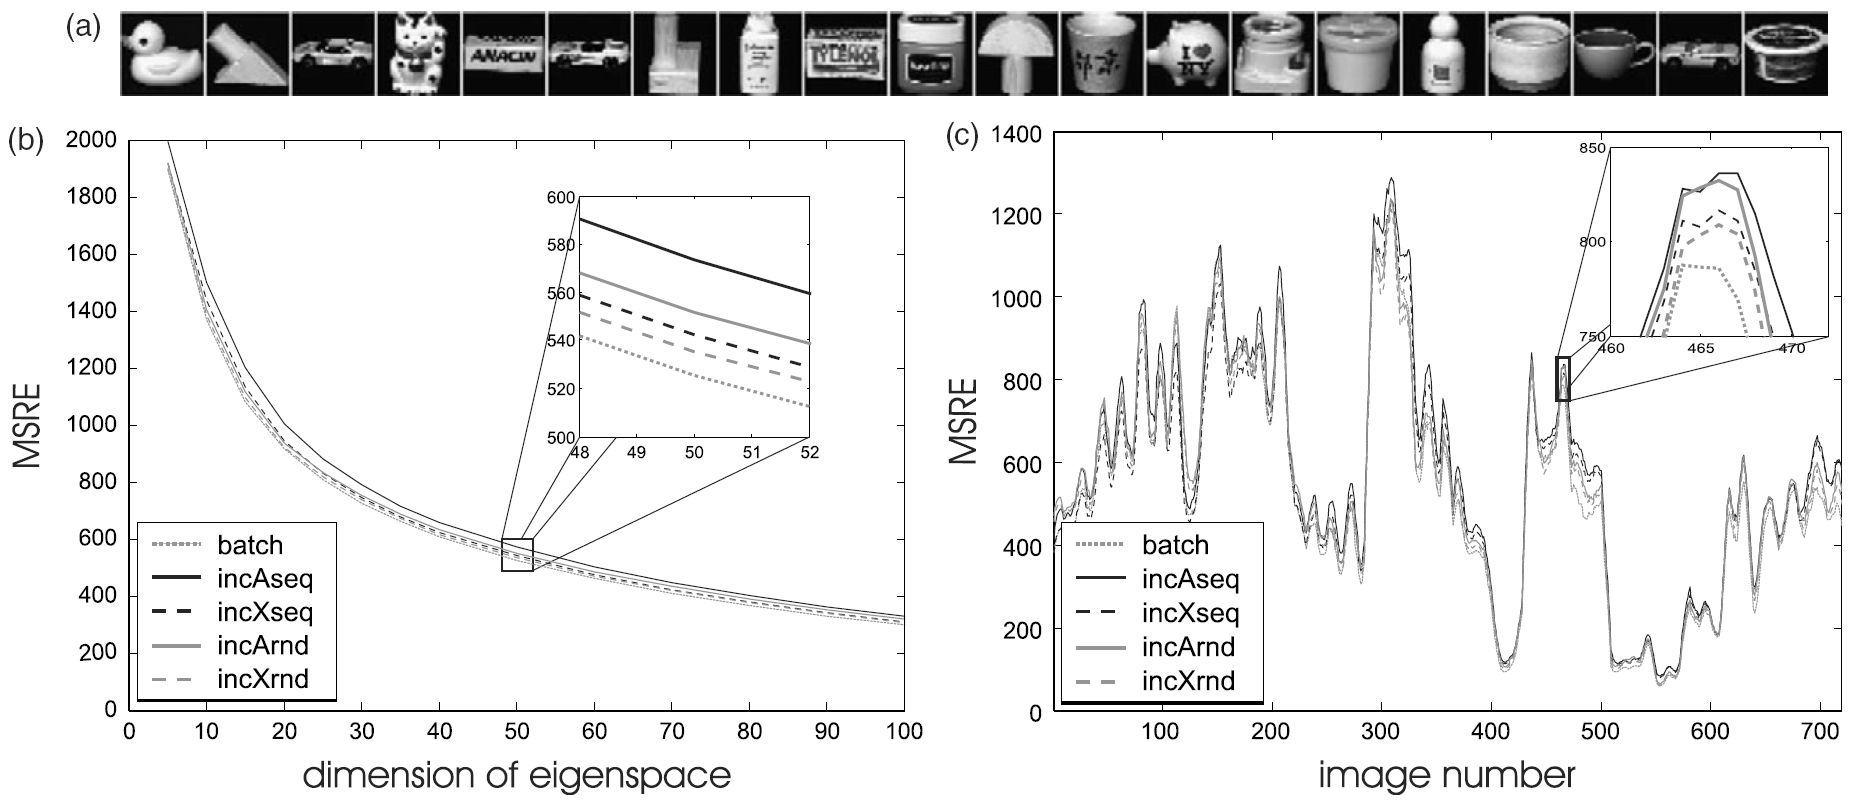
\includegraphics[width=1.0\textwidth]{figs/2008_JNL_TRKsub_Skocaj_fig4.png}}
								\subfigure[Comparison of weighted vs non-weighted batch and incremental PCA algorithms]{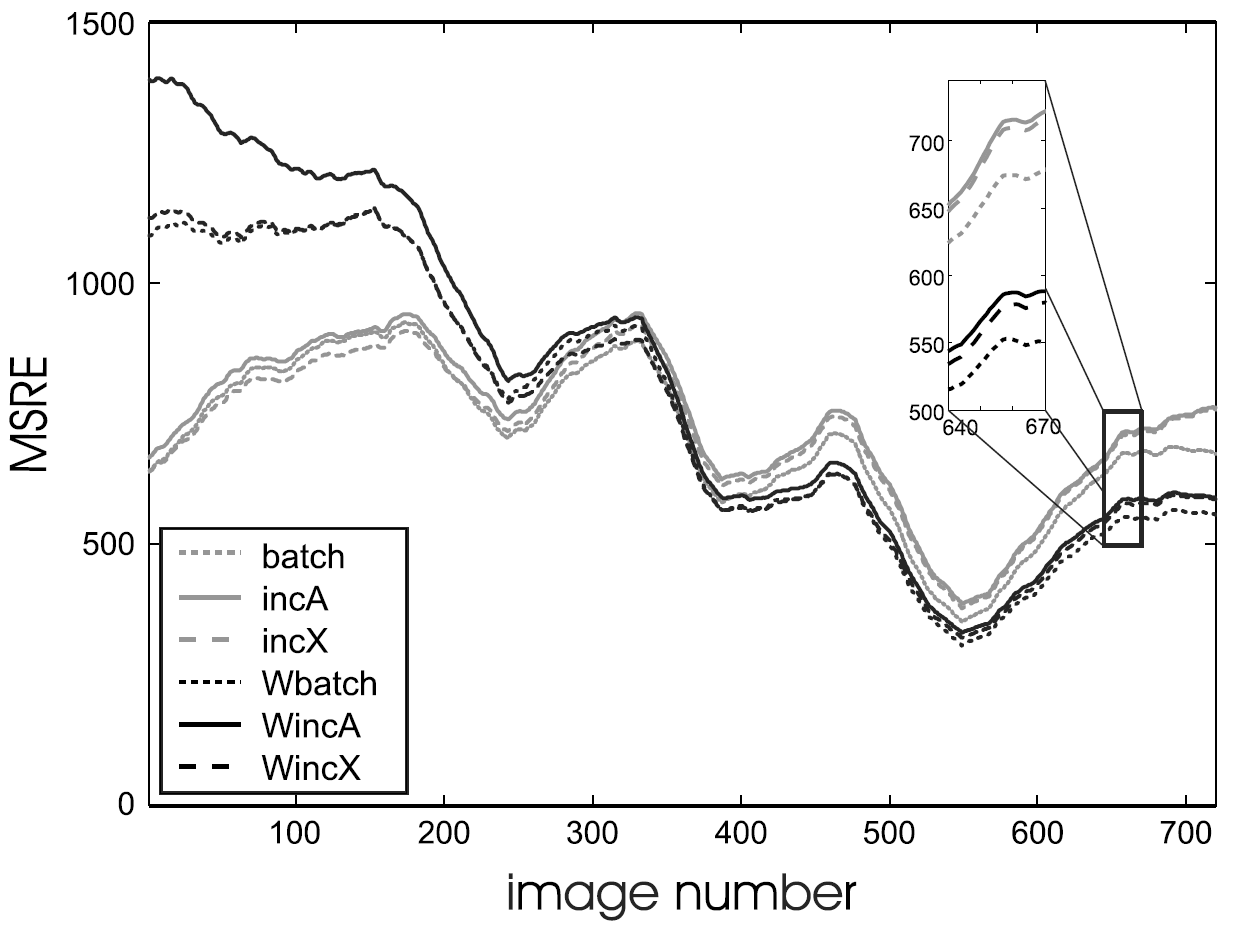
\includegraphics[width=0.5\textwidth]{figs/2008_JNL_TRKsub_Skocaj_fig5.png}}
								\caption{Comparison of batch PCA with various incremental PCA update algorithms \cite{2008_JNL_TRKsubs_Skocaj}}
								\label{fig:2008_JNL_TRKsub_Skocaj}				
								\end{figure}

\cite{2008_JNL_TRKsubs_Skocaj} try to find the error associated with using an incremental PCA update algorithm versus using the optimal batch PCA algorithm.  They build eigenspaces of various dimensions from 720 images of 20 objects taken from the Columbia University Image Library (COIL-100)  \cite{Web_COIL}.  Figure~\ref{fig:2008_JNL_TRKsub_Skocaj} shows the mean squared reconstruction errors (MSRE) for the batch and various incremental methods.  In all experiments, squared reconstruction error degradation is less than 10\%.  Moreover, the sequential order in which the images are presented influences results.  It is pointed out that to obtain good results, the initial images should be heterogenous encompassing different objects and views.  This results in an evolving eigenspace that is rich and comprehensive enough in the beginning and is not specialized for representing a specific object only.  In this work, it is also shown that the reconstruction errors of the various incremental weighted PCA methods (\emph{WincA, WincX}) do not differ significantly from the results of the batch weighted method (\emph{Wbatch}).  This method is used by \cite{2010_CNF_TRKsubs_Qian} for object tracking in a manner quite similar to the approach used in \cite{2008_JNL_subspaceTRK_Ross}.  They sample a collection of image patches and likelihood of each image patch is generated by reconstruction.  Comparison is made between PCA subspace tracking with and without weighting prior observations.  They show that temporal weighting the data results in less background clutter penetrating the target of interest and therefore leads to better occlusion handling in tracking.  Another incremental PCA update algorithm is developed by \cite{2004_JNL_TRKsubs_Li}.  They also propose an incremental algorithm robust PCA in addition to standard PCA.

Having discussed traditional and subspace based tracking methods, we now turn to the usage of RVQ in tracking.


%								\begin{figure}[t]
%								\center
%								\includegraphics[width=0.5\textwidth]{figs/PRML_hierarchy_Bayes_MRF_regularization.pdf}
%								\caption{Splines are equivalent to standard (smoothness based) regularization.  Standard regularization is a special case of MRF models.  MRF models are a subset of Bayesian estimators \cite{1990_JNL_Network_Poggio}}
%								\label{fig:PRML_hierarchy_Bayes_MRF_regularization}
%								\end{figure}

%@@@@@@@@@@@@@@@@@@@@@@@@@@@@@@@@@@@@@@@@@@@@@@@@@@
\chapter{Visual Tracking Using RVQ}
\label{chap_RVQ_TRK}	
%@@@@@@@@@@@@@@@@@@@@@@@@@@@@@@@@@@@@@@@@@@@@@@@@@@
%===================
\section{Introduction}
%===================
A learning-based tracking framework builds the target model while it tracks, thus avoiding the costly step of building target models prior to tracking.  This has been demonstrated successfully for PCA based tracking using publicly-available challenging datasets.  In this work, we use Residual Vector Quantization in a learning-based tracking framework using the same datasets and show that RVQ performs as well as PCA.  Moreover, we introduce 2 new distance metrics for relative weighting of target candidates allowing RVQ to be used as a generative model, similar to the way probabilistic PCA converts PCA into a generative framework.

In this chapter, we combine information on target representations presented in Chapter~\ref{chap_Introduction}, theoretical knowledge of RVQ presented in Chaper~\ref{chap_RVQ} and an overview of tracking methods presented in Chapter~\ref{chap_TRK} into a visual tracking framework using RVQ and compare it with visual tracking using PCA and TSVQ.  

This work is significant since PCA is commonly used in the Pattern Recognition, Machine Learning and Computer Vision communities.  On the other hand, TSVQ is commonly used in the Signal Processing and Information Theory communities.  RVQ with more than two stages has not received much attention due to the difficulty in producing stable designs.  In this work, we bring together these different approaches and compare them in a combined visual tracking framework.  The result is a robust tracker for all 3 methods, but with RVQ performing the best according to certain defined criteria to be described later in the chapter.

The approach we take in this work builds on work presented by Ross et. al. in 2008 \cite{2008_JNL_subspaceTRK_Ross}.  As a matter of fact, we have used part of their software with their permission~\cite{2008_SFT_Ross}.  In this spirit, we make our software available for download to the community at \url{https://github.com/SalmanAslamPhD/current}.  

%----------------------------------------
\subsection{Challenges}
%----------------------------------------
Visual tracking is the task of estimating a target's state over time.  In many cases, the state represents target position and a bounding box around it, or its contour.  However, this is a challenging problem due to the following reasons:

\begin{enumerate}
\item \underline{Appearance and contour changes}:  A target of interest can undergo arbitrary change in appearance and contour.  This can be due to the following reasons:
\begin{enumerate}
\item \underline{Pose change}:  The target can rotate and present a different view to the camera.
\item \underline{Warping}: The target can undergo warps, such as expression changes for humans.
\item \underline{Self occlusion}:  The target can be occluded or unoccluded by itself or its surroundings.
\item \underline{Blur}:  Motion blur can severely distort a target's appearance.
\item \underline{Structured noise}:  The target can change appearance in an orderly manner, for instance, a target of interest can put on or remove glasses or a hat.
\item \underline{Random noise}:  Random noise is added to the light rays coming from a target of interest.  On the hardware side, this is caused by atmospheric effects in the optical channel.  On the receiving side, it is caused by sensor noise, electronics noise and EMI (electromagnetic interference).  On the software side, it can be caused by compression artefacts.
\item \underline{Non-symmetic BRDF}:  The light reflected off of an object in all directions is modeled by the BRDF (Bidirectional Radiation Transfer Function).  Since this function may not be symmetric in all directions, the amount of light reflecting off of the object may be different in different directions.  Multiple cameras viewing the same point will receive different intensity levels.
\end{enumerate}
\item \underline{Lighting change}: Lighting changes can be caused by turning on or off lights in indoor environments, or moving into or out of shades in outdoor environments.
\item \underline{Sudden motion (target or camera)}:  Besides motion blur, sudden motion by the target or camera can cause the target to exit the window in which the tracker looks for the target leading to incorrect track assignment.
\end{enumerate}

For a tracker that tries to learn the appearance and/or contour model of the target, inclusion of background pixels is an added problem that can cause drift.  If none of the problems mentioned above were present, a simple template matching stategy would suffice for robust tracking.  This has complexity $O(nm)$, where $n$ is the number of pixels in the target and $m$ is the number of locations at which the target is searched.  For most practical situations, this does not represent significant computational load and can be done in real time even while tracking several targets.
								\begin{figure}[t]
								\centering
								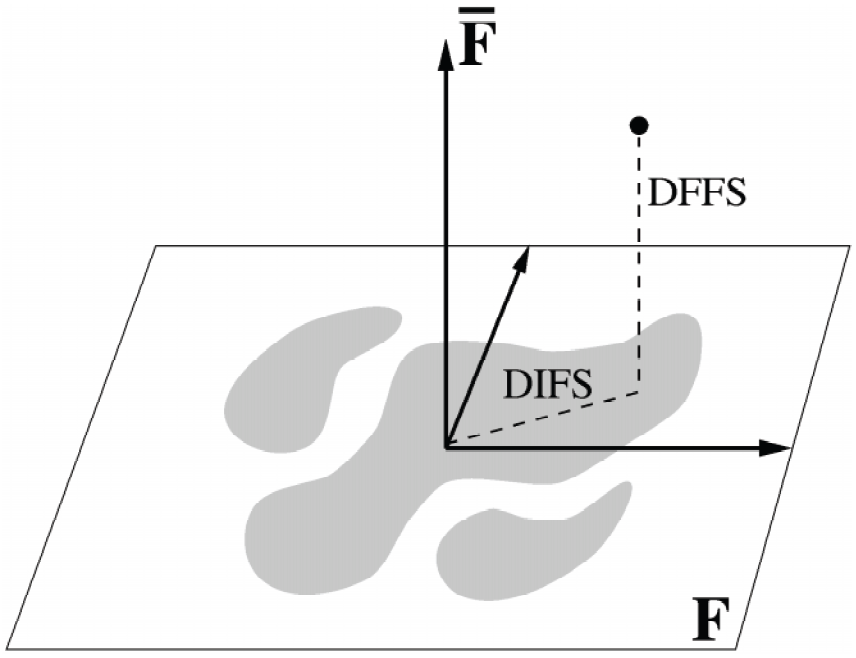
\includegraphics[width=0.5\textwidth]{thesis/1998_JNL_ProbVisLearning_Moghaddam_fig3.png}
								\caption{Graphical illustration of DFFS (distance-from-feature-space) and DIFS (distance-in-feature-space).  The feature space is $\mathbf{F}$ while the subspace orthogonal to the feature space is $\bar{\mathbf{F}}$.  DFFS is the signal residual error and DIFS is the $\mathbf{F}$-space likelihood \cite{1997_JNL_EigenTRK_Moghaddam}.}
					\label{fig:1997_JNL_DIFSDFFS_Moghaddam}
								\end{figure}


%----------------------------------------
\subsection{Brief history}
%----------------------------------------
In this work, we try to address single-target visual-tracking under several of the challenges mentioned above while trying to learn the appearance model of the target.  Seminal work here can be traced back to 1996 when Black and Jepson experimented with tracking using an eigenspace representation of the target appearance model~\cite{1998_JNL_Eigentracking_Black}.  The next notable work is by Moghaddam and Pentland, 1997~\cite{1997_JNL_EigenTRK_Moghaddam} in which they try to address a fundamental limitation of PCA.  In PCA, 2 vectors, $\mathbf{x}_1$ and $\mathbf{x}_2$ can have the same distance to a reduced eigenspace even if they have different distance to the mean of the data.  This is shown for a trivial case in $\mathbb{R}^2$ in Figure~\ref{fig:PRML_PCA_problem} where $\mathbf{e}_1=\mathbf{e}_2=\mathbf{e}$ even though $\mathbf{x}_1$ is closer to the mean $\boldsymbol\mu$ than $\mathbf{x}_2$.  They formulate the problem using DIFS (distance in feature space) and DFFS (distance from feature space) so that both projection error and distance to the mean of the data are used while trying to determine how well the subspace explains a new data-point.  The next breakthrough came with the work of Bishop and Tipping in 1999~\cite{1999_JNL_PPCA_Tipping} where they show that a probabilistic variation of PCA (PPCA) allows PCA to be used as a generative model.  The advantage in tracking is that this methodology allows an assignment of probabilities to new data-points.  This relative weighting can be used to determine best candidates.  All three works were combined into a tracking framework for the first time by Ross et. al. in 2008~\cite{2008_JNL_subspaceTRK_Ross}.  Moreover, they used incremental SVD to make their tracker run in real time.  

Here, we extend this work using RVQ instead of PCA and introducing two new distance based measures for relative weighting of tracking candidates.  The result is a generative framework for RVQ that leads to robust tracking.  Whereas RVQ was first introduced by Juang and Gray in 1982~\cite{1982_CNF_SpeechRVQ_JuangGray}, subsequently greatly extended by the seminal work of Barnes~\cite{1991_CNF_DesignPerformanceRVQ_Frost,1992_JNL_RVQ_Barnes,1992_CNF_ImageCodingRVQ_Kossentini,1993_sigmaTrees_Barnes,1993_JNL_RVQDSC_Barnes,1995_JNL_OptimalityRVQ_Kossentini,1996_CNF_VQclassification_Barnes,1996_JNL_AdvancesRVQ_Barnes,2002_JNL_SigmaTrees_Barnes,2004_CNF_DSSAdataMining_Barnes,2007_JNL_Katrina_Barnes,2007_JNL_IDDM_Barnes} and widely known in the signal processing and information theory communities, relatively little attention has been given to this work in the computer vision and machine learning fields where a much simpler version, K-means, has been widely used.  Our goal is to remedy this situation and introduce RVQ in the context of an important and challenging problem, visual target tracking.

								\begin{figure}[t]
								\centering
	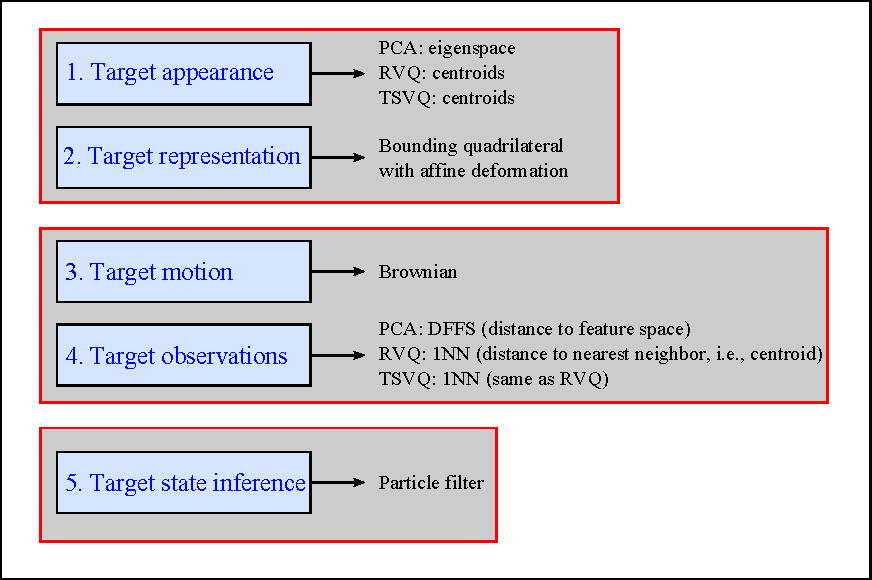
\includegraphics[width=1.0\textwidth]{thesis/PhD_experimentalOverview.pdf}
								\caption{Overview.}
								\label{fig:overview}
								\end{figure}

								\begin{figure}[t]
								\centering
								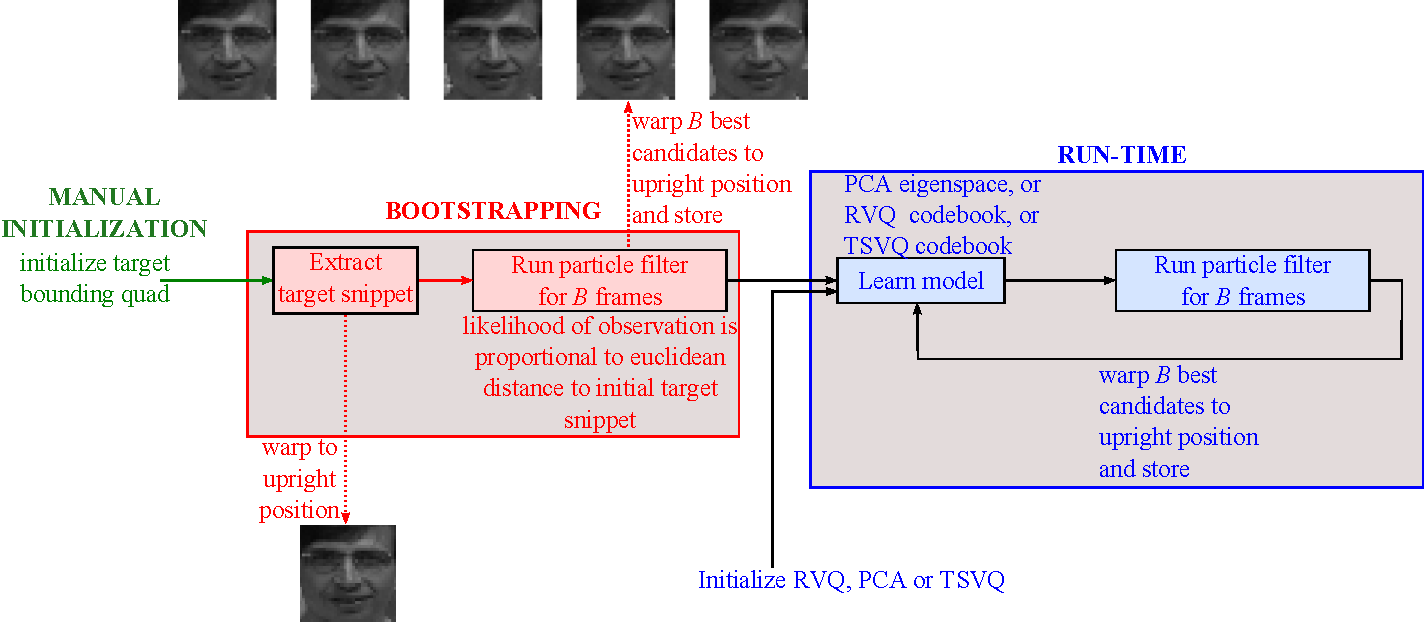
\includegraphics[width=1\textwidth]{thesis/PhD_experimentalTemporalOverview.pdf}
								\caption{Temporal overview.}
								\label{fig:temporal_overview}
								\end{figure}
%----------------------------------------------------
\subsection{Overview of approach used}
%----------------------------------------------------
Our tracking framework is based on five components as shown in Figure~\ref{fig:overview} .  Each of these components is described in detail in later sections.  Here, we present an overview of each:

\begin{enumerate}
\item \underline{ Target appearance}.  Target appearance is modeled using a learned eigenspace, a trained $\sigma$-tree codebook or a binary balanced-tree TSVQ codebook for PCA, RVQ and TSVQ respectively.  Refer to Chapter~\ref{chap_RVQ} for a description of RVQ  $\sigma$-trees.

\item \underline{Target representation}.  Several target representation methods are described in Chapter~\ref{chap_Introduction}.  We use the bounding quadrilateral method.  This quad encloses the pixels of a target of interest.  It is also allowed to warp affinely from frame to frame to minimize inclusion of background pixels as the target changes shape, size and orientation.

\item \underline{Target motion}.  In order to keep our work general, we do not assume any deterministic target motion model.  The target is expected to move according to a Wiener process, i.e., brownian motion.  This allows for robust tracking under arbitrary target and camera motion.

\item \underline{Target observations}.  For PCA, the likelihood of a target observation is assumed proportional to the DFFS (distance to feature space).  DFFS is explained in Chapter~\ref{chap_TRK}.  For RVQ, the likelihood of a target observation is assumed to be proportional to the Euclidean distance to the closest equivalent code-vector.  Equivalent code-vectors are explained in Chapter~\ref{chap_RVQ}.  For TSVQ, the likelihood of a target observation is assumed to be proportional to the Euclidean distance to the closest terminal code-vector.

\item \underline{Target state inference}.  In tracking, the correspondence of observations in the current frame to existing targets in the previous frame is generally an ill-posed problem~\cite{2005_CNF_TRK_Yang}.  We use the particle filter to deal with this problem by propagating multiple hypotheses from frame to frame~\cite{1998_JNL_Condensation_IsardBlake}.

\end{enumerate}

%----------------------------------------------
\subsection{Overview of temporal process}
%----------------------------------------------
In the previous section, we described the five major components of our visual tracking framework.  In this section, we describe the temporal relationship between these components.  Refer to Figure~\ref{fig:temporal_overview} for a graphical overview.  A brief description of this temporal process is given below while detailed explanation is given in later sections in this chapter.

\begin{enumerate}
\item \underline{Manual initialization}.  The target is identified in the first frame by manually drawing a bounding box around it.

%The box is allowed to be affinely deformed as discussed later in this chapter.  Template matching then allows a certain number of frames to be designated as initial training frames.  Currently this value is set to $N_B=5$. 

\item \underline{Bootstrapping}.  A particle filter is run for $B$ frames.  The likelihood of observations is assumed to be proportional to the Euclidean distance from the manually segmented target in the first frame.  The $B$ MAP estimates, i.e. $B$ snippets, one from each of the $B$ frames is stored.

  \item \underline{Run-time}.  During this step, the learning process and the particle run alternately.  For PCA, the learning process includes updating its eigenbasis with the MAP estimates of the particle filter.  For RVQ and TSVQ, the learning process includes updating their codebooks. 
\end{enumerate}


%This model ties in multiple possible spatial observations in a temporal framework to enable sequential inference through the tracking process.
%Every frame after the one-time initialization is tested against the iPCA, bPCA, RVQ and TSVQ models and results are compared.  The Condensation algorithm is used for temporal and spatial integration of observation and state information.  Spatial processing includes generating several candidate window chips (snippets) and picking the one that gives least mean squared reconstruction error.  Temporal processing includes carrying over the posterior density from a frame as the prior density for the next frame.  The snippet that gives the least squared error is retained and added to the pool of training images in FIFO (first-in first-out) fashion, i.e. a moving window of $N_w$ training images is maintained.

The integration of the above-mentioned 5 components in the temporal process just explained enables us to handle the following tracking challenges:

\begin{itemize}
\item \underline{Target appearance related}: Target pose changes, lighting changes, structured noise and temporary occlusions.
\item  \underline{Target representation related}: Target scale and orientation changes.
\item  \underline{Target motion related}: Arbitrary camera and target motion.
\end{itemize}

We now discuss each component in our tracking framework (Figure~\ref{fig:overview}).  

%============================
\section{Model 1: Appearance model}
\label{Sec:RVQ_trk_appearance_model}
%============================
\begin{figure}[t]
\subfigure[Uniform random variable $U\sim$ \texttt{[}0, 1\texttt{]} in $\mathbb{R}^{1089}$, 100 realizations.]{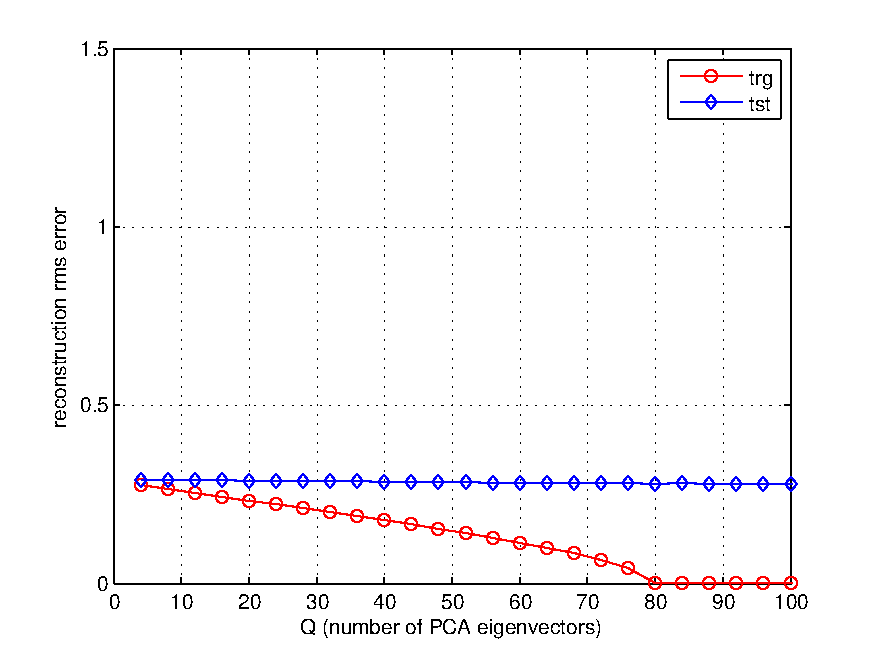
\includegraphics[width=0.45\textwidth]{thesis/PCA_Uniform.pdf}}
\subfigure[Gaussian random variable $\mathcal{N}\sim$(0, 1) in $\mathbb{R}^{1089}$, 100 realizations.]{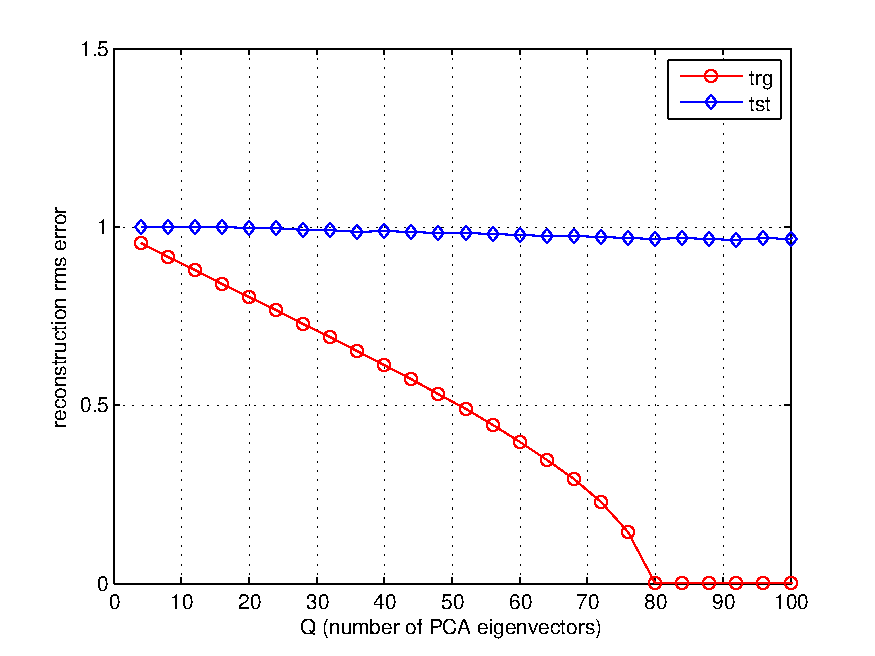
\includegraphics[width=0.45\textwidth]{thesis/PCA_Gaussian.pdf}}
\subfigure[Gauss-Markov random variable $\mathcal{N}\sim$(0, 1) in $\mathbb{R}^{1089}$ with 0.9 correlation, 100 realizations.]{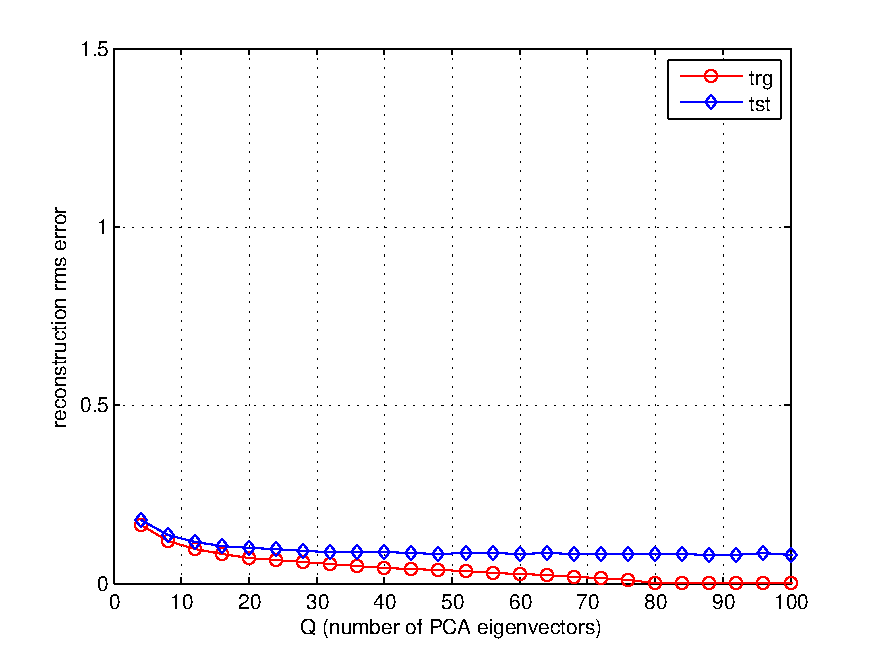
\includegraphics[width=0.45\textwidth]{thesis/PCA_GaussMarkov.pdf}}\hspace{0.55in}
\subfigure[Dudek sequence, 33x33 ($\mathbb{R}^{1089}$) face snippets were extracted from the first 100 images.]{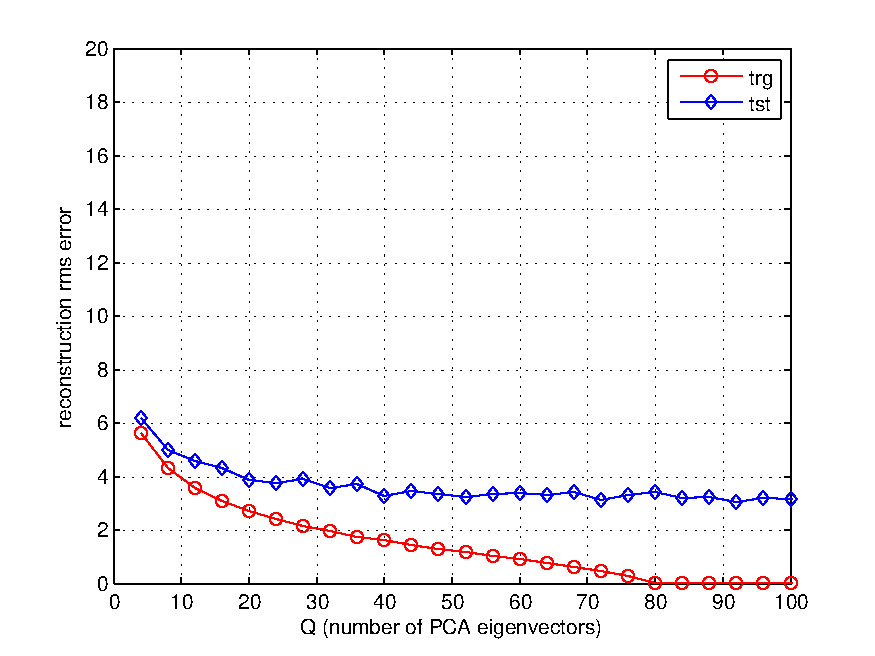
\includegraphics[width=0.45\textwidth]{thesis/PCA_Dudek.pdf}}
\caption{PCA, 100 training examples in $\mathbb{R}^{1089}$ were used for each of these experiments. Results were averaged over 10 cross-validation runs. For each run, 20\% of the data, i.e., 20 examples were randomly picked for testing while the remaining 80 examples were used for training.}
\label{fig:PCA_results}
\end{figure}

\begin{figure}[t]
\subfigure[Uniform random variable $U\sim$ \texttt{[}0, 1\texttt{]} in $\mathbb{R}^{1089}$, 100 realizations.]
{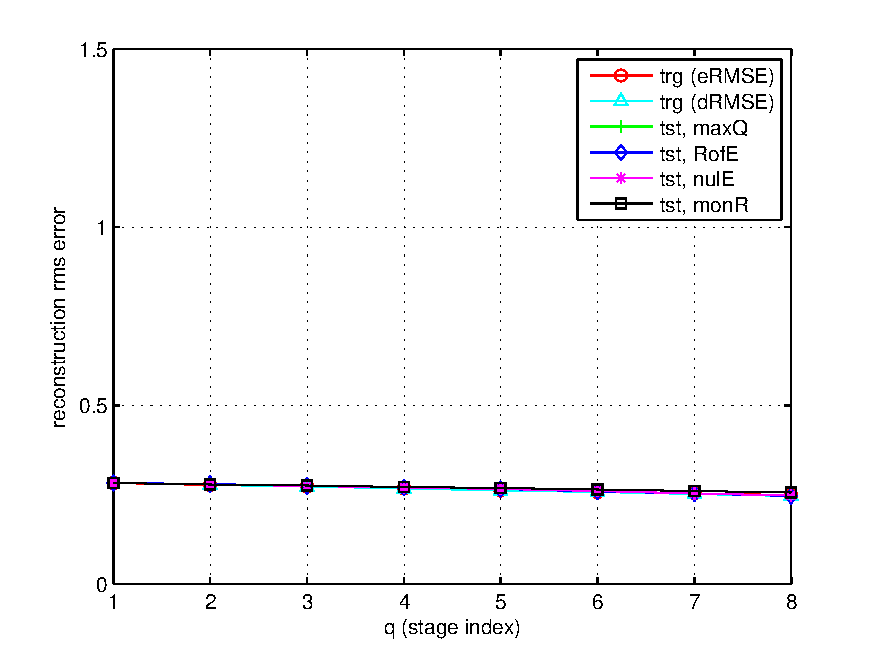
\includegraphics[width=0.45\textwidth]{thesis/RVQ_8x4_Uniform.pdf}}
\subfigure[Gaussian random variable $\mathcal{N}\sim$(0, 1) in $\mathbb{R}^{1089}$, 100 realizations.]
{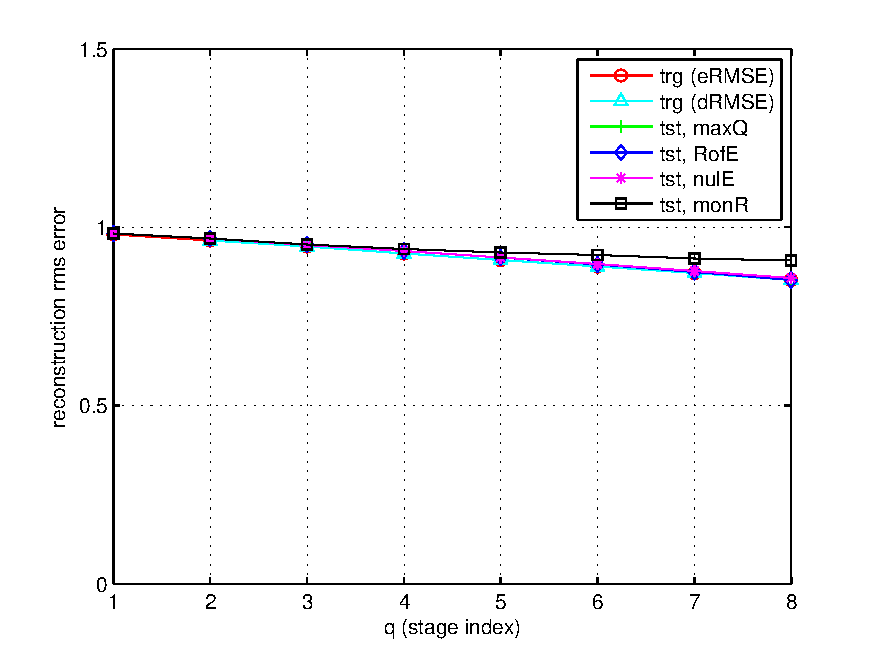
\includegraphics[width=0.45\textwidth]{thesis/RVQ_8x4_Gaussian.pdf}}
\subfigure[Gauss-Markov random variable $\mathcal{N}\sim$(0, 1) in $\mathbb{R}^{1089}$ with 0.9 correlation, 100 realizations.]
{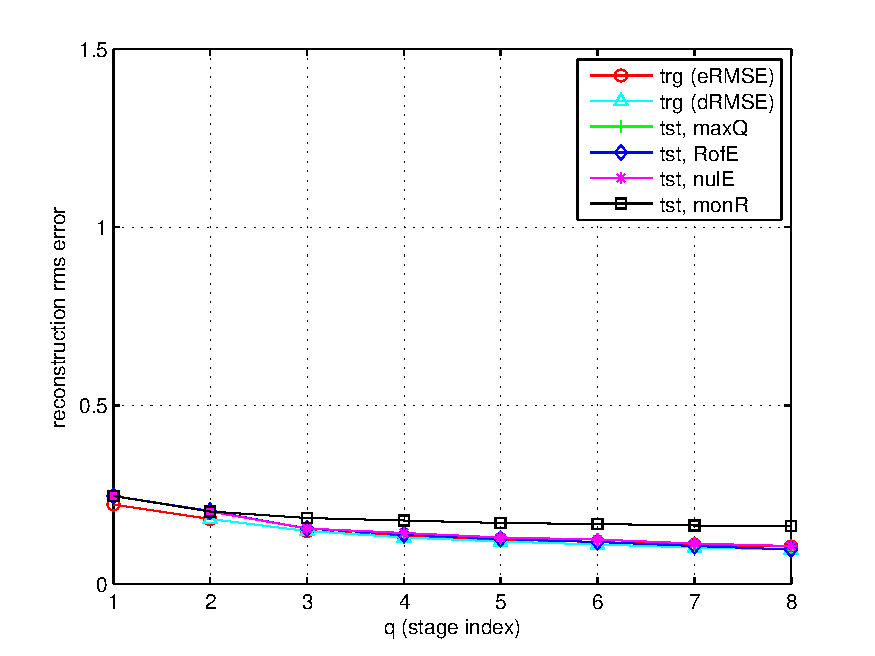
\includegraphics[width=0.45\textwidth]{thesis/RVQ_8x4_GaussMarkov.pdf}}\hspace{0.55in}
\subfigure[Dudek sequence, 33x33 ($\mathbb{R}^{1089}$) face snippets were extracted from the first 100 images.]
{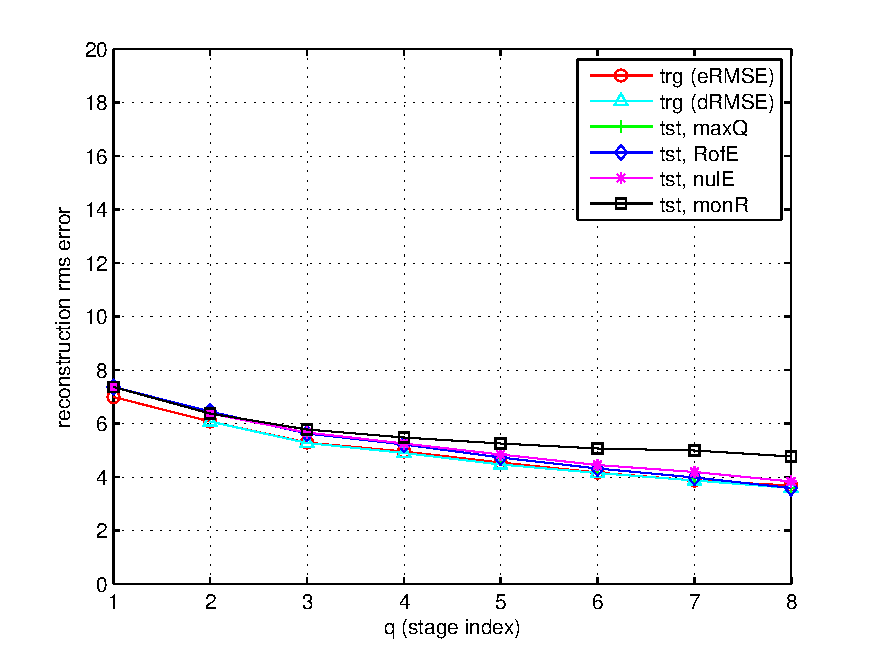
\includegraphics[width=0.45\textwidth]{thesis/RVQ_8x4_Dudek.pdf}}
\caption{RVQp, varying number of stages $P$ with number of code-vectors per stage held constant at $M=4$. 100 training examples in $\mathbb{R}^{1089}$ were used for each of these experiments. A single test example in $\mathbb{R}^{1089}$ was reconstructed.}
\label{fig:RVQ_results_varyingP}
\end{figure}

\begin{figure}[t]
\subfigure[Uniform random variable $U\sim$ \texttt{[}0, 1\texttt{]} in $\mathbb{R}^{1089}$, 100 realizations.]
{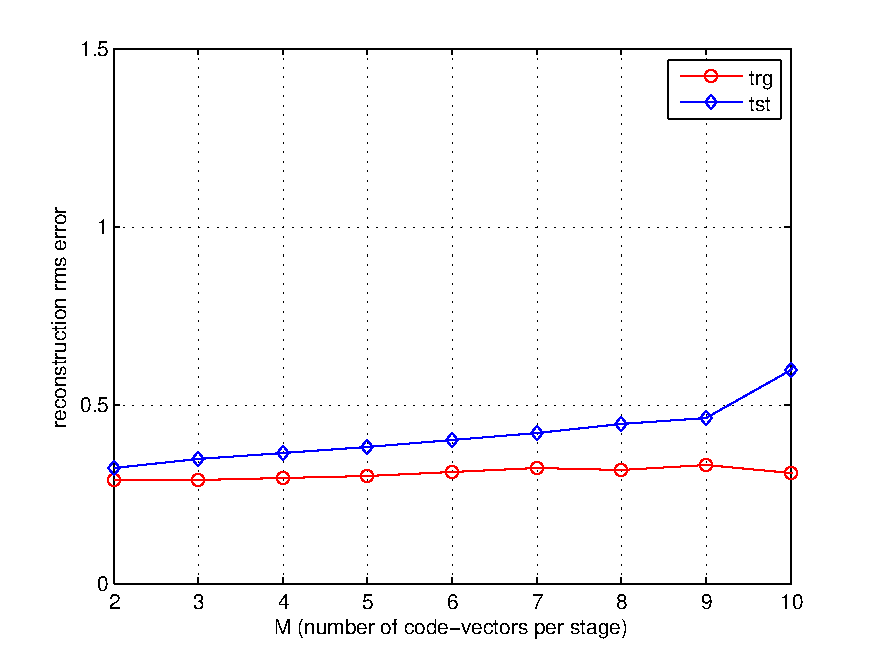
\includegraphics[width=0.45\textwidth]{thesis/RVQ_uniform.pdf}}
\subfigure[Gaussian random variable $\mathcal{N}\sim$(0, 1) in $\mathbb{R}^{1089}$, 100 realizations.]
{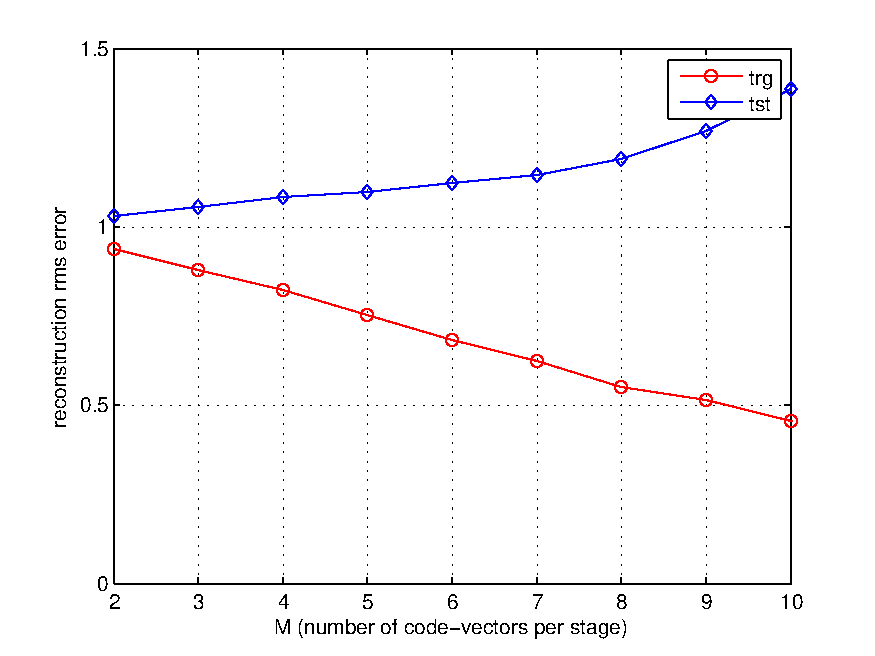
\includegraphics[width=0.45\textwidth]{thesis/RVQ_Gaussian.pdf}}
\subfigure[Gauss-Markov random variable $\mathcal{N}\sim$(0, 1) in $\mathbb{R}^{1089}$ with 0.9 correlation, 100 realizations.]
{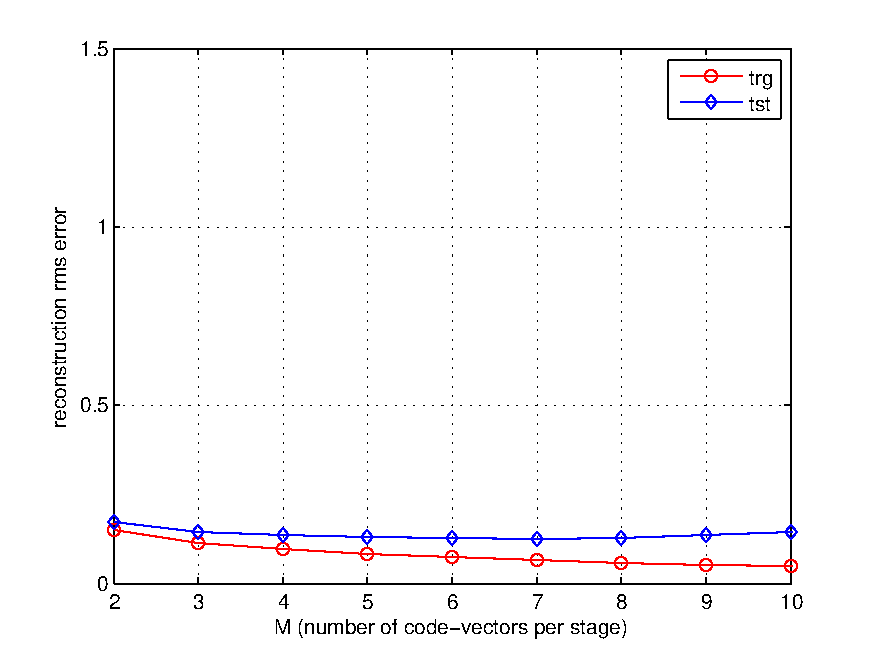
\includegraphics[width=0.45\textwidth]{thesis/RVQ_GaussMarkov.pdf}}\hspace{0.55in}
\subfigure[Dudek sequence, 33x33 ($\mathbb{R}^{1089}$) face snippets were extracted from the first 100 images.]
{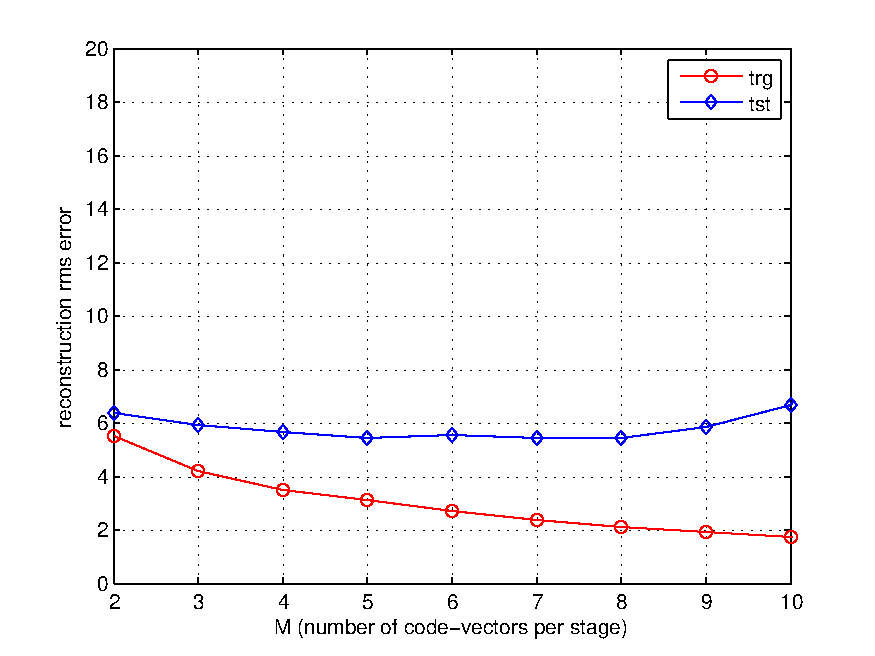
\includegraphics[width=0.45\textwidth]{thesis/RVQ_Dudek.pdf}}
\caption{RVQm, experiments, varying number of code-vectors per stage $M$ with number of stages held constant at $P=8$. 100 training examples in $\mathbb{R}^{1089}$ were used for each of these experiments. Results were averaged over 10 cross-validation runs. For each run, 20\% of the data, i.e., 20 examples were randomly picked for testing while the remaining 80 examples were used for training.}
\label{fig:RVQ_results_varyingM}
\end{figure}

\begin{figure}[t]
\subfigure[Uniform random variable $U\sim$ \texttt{[}0, 1\texttt{]} in $\mathbb{R}^{1089}$, 100 realizations.]{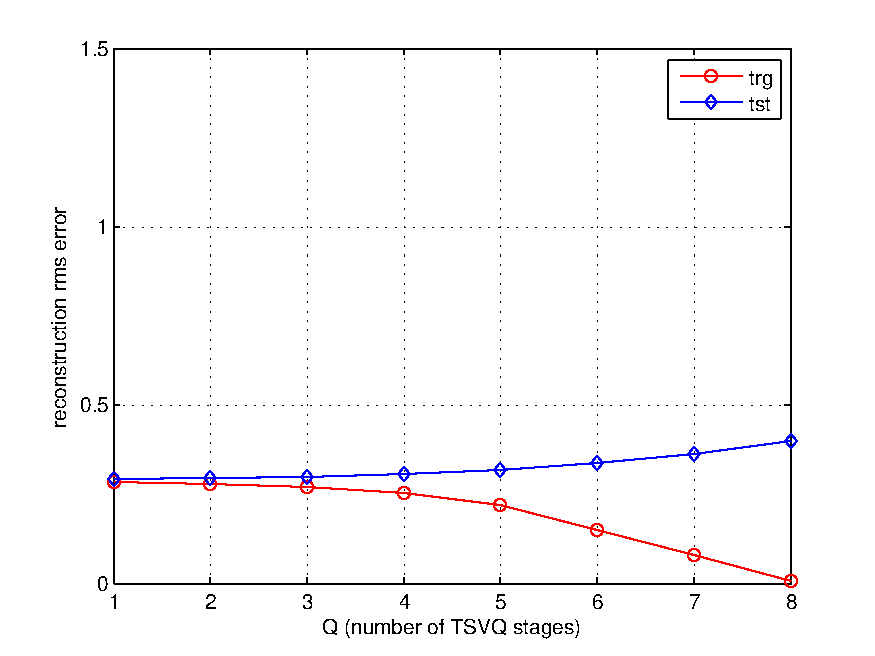
\includegraphics[width=0.45\textwidth]{thesis/TSVQ_Uniform.pdf}}
\subfigure[Gaussian random variable $\mathcal{N}\sim$(0, 1) in $\mathbb{R}^{1089}$, 100 realizations.]{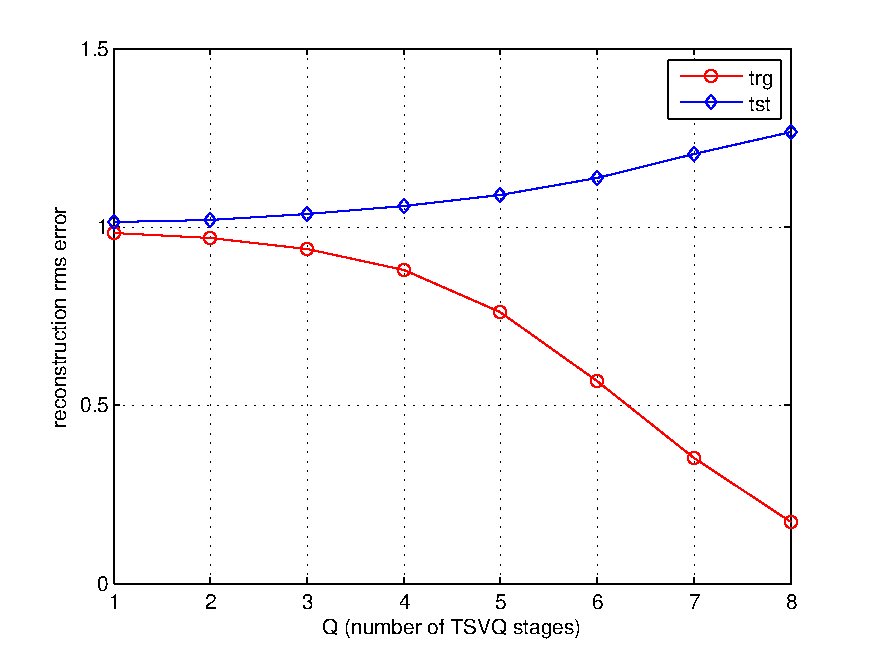
\includegraphics[width=0.45\textwidth]{thesis/TSVQ_Gaussian.pdf}}
\subfigure[Gauss-Markov random variable $\mathcal{N}\sim$(0, 1) in $\mathbb{R}^{1089}$ with 0.9 correlation, 100 realizations.]{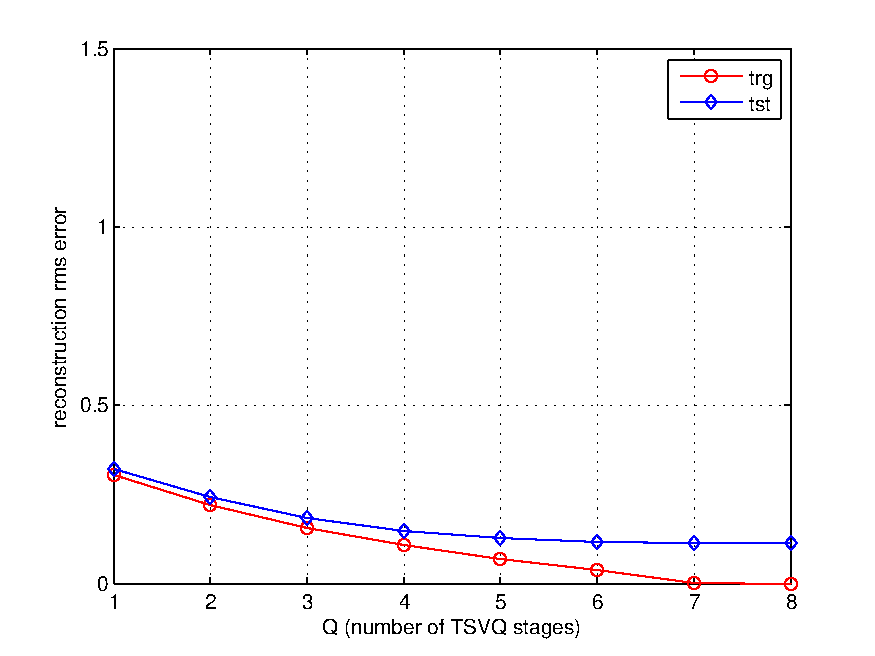
\includegraphics[width=0.45\textwidth]{thesis/TSVQ_GaussMarkov.pdf}}\hspace{0.55in}
\subfigure[Dudek sequence, 33x33 ($\mathbb{R}^{1089}$) face snippets were extracted from the first 100 images.]{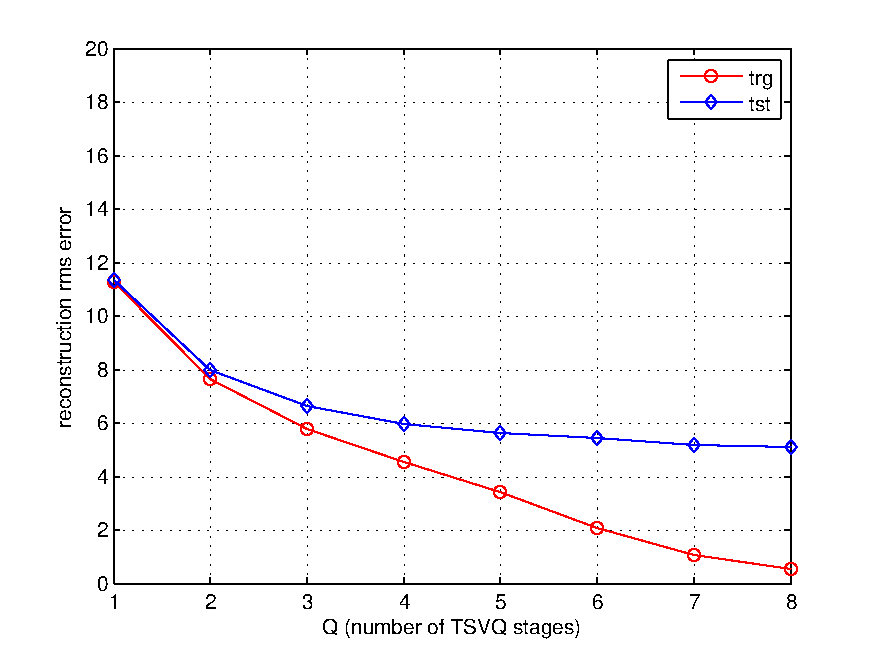
\includegraphics[width=0.45\textwidth]{thesis/TSVQ_Dudek.pdf}}
\caption{TSVQ, 100 training examples in $\mathbb{R}^{1089}$ were used for each of these experiments. Results were averaged over 10 cross-validation runs. For each run, 20\% of the data, i.e., 20 examples were randomly picked for testing while the remaining 80 examples were used for training.}
\label{fig:TSVQ_results}
\end{figure}

Common appearance models include just the raw values of the pixel intensities~\cite{2000_CNF_TRK_Mallet, 1981_JNL_OpticalFlow_HornSchunck}, pixel intensity distributions~\cite{2002_JNL_MeanShiftFeatureSpaceAnalysis_Comaniciu, 1996_JNL_TRK_Zhu, 2002_JNL_TRK_Paragios, 2002_JNL_TRK_Elgammal}, templates\cite{1997_CNF_TRK_Fieguth}, active appearance models\cite{1998_CNF_ActiveModels_Edwards, 1995_JNL_ActiveModels_Cootes}, pixel intensity centroids~\cite{1997_CNF_TRK_Heisele} and subspace based methods~\cite{1997_JNL_EigenTRK_Moghaddam, 1998_JNL_Eigentracking_Black}.  

In order to understand appearance modeling, we conduct the following 4 experiments using PCA, RVQ and TSVQ to measure rms errors for target reconstruction:

\begin{enumerate}
\item PCA: varying number of eigenvectors, $Q$.
\item RVQp: varying number of stages $P$ for RVQ while holding the number of code-vectors per stage constant at $M=4$.
\item RVQm: varying number of code-vectors per stage for RVQ while holding the number of stages constant at $P=8$.
\item TSVQ: varying number of stages, $P$.
\end{enumerate}

It is hoped that investigating reconstruction errors will aid in understanding the behavior of these various algorithms when used to model target appearance in tracking applications.

We use four datasets in $\mathbb{R}^{1089}$: (a) Uniform random variable, (c) Gaussian random variable, (c) Gauss-Markov random variable, and (d) images from the Dudek sequence. The reason for using $\mathbb{R}^{1089}$ is that our targets for all our tracking datasets are warped to a canonical size of 33-pixel height and 33-pixel width (33x33=1089). In all cases, we take 100 examples and split them up using an 80/20 rule, i.e. 80 training examples and 20 test examples. 10 cross-validation runs are used. In each cross-validation run, the training and test examples are picked randomly in the 80/20 ratio.

Results for PCA, RVQp, RVQm and TSVQ are shown in Appendix~\ref{App:plots} as Figures~\ref{fig:PCA_results}, \ref{fig:RVQ_results_varyingP} \ref{fig:RVQ_results_varyingM} and \ref{fig:TSVQ_results} respectively.
We make the following observations from the results:
\begin{enumerate}
\item \textbf{Training error}. Training error is always less than test error, as expected. Also, for each of the algorithms individually, we observe,
\begin{itemize}
\item \underline{PCA}: Monotonic decrease with increasing $Q$. Training error becomes 0 when 80 eigenvectors are used, since there are 80 training examples.
\item \underline{RVQp}: Monotonic decrease with increasing $P$.
\item \underline{RVQm}: Can increase or decrease with increasing $M$, but slight variation.
\item \underline{TSVQ}: Monotonic decrease with increasing $P$.
\end{itemize}
\item \textbf{Test error}.
\begin{itemize}
\item \underline{Statistically independent data}: For the uniform and Gaussian random variables, test error for PCA and RVQp stays almost constant with increasing $Q$ and $P$ respectively. For RVQm and TSVQ, test error increases with increasing $P$. The reason is that PCA and RVQp use successive refinement when increasing $Q$ and $P$ respectively. Test error is therefore not expected to get better since it is not possible to better explain random data with increasing $Q$ and $P$.
On the other hand, RVQm and TSVQ control generalization ability with increasing $Q$, as discussed in an earlier report on VC dimension. Therefore, when the number of code-vectors increases, they tend to explain the training data well and are unable to explain the test data. For both RVQm and TSVQ, notice that when training error falls off sharply, test error increases sharply. Also, when training error drop is gradual, so is test error increase rate. This confirms over-generalization behavior. Also, RVQ increase or decrease rates are more gradual than TSVQ. And finally, the over-generalization for both RVQm and TSVQ is less pronounced with uniform random data than with Gaussian random data since there is more uncertainty in the latter distribution.
\item \underline{Statistically dependent data}: For the Gauss-Markov and Dudek cases, all 4 algorithms display decreasing test error with increasing $Q$ or $P$. The "knee" is visible in all cases.
\end{itemize}
\end{enumerate}
In general, the training and test errors for RVQ are less than TSVQ. This is due to the fact that RVQ has access to all data at every stage while designing codebooks, and can therefore better optimize stage code-vectors. In TSVQ, data is partitioned at every stage and can lead to data starvation.
Training error of PCA is in general better than RVQ. This is expected since PCA can achieve perfect reconstruction when $Q$ comes close to the number of training examples $N$, $N<<D$. Test errors however are comparable.

RVQ has 2 knobs, $P$ and $M$. In varying $P$, it acts like PCA in providing successive approximation. In varying $M$, it acts like TSVQ in changing its VC dimension, and therefore its generalization ability.
Given this flexibility, it is expected that RVQ will perform well in tracking experiments.

%=======================		
\section{Model 2: Observation model}
%=======================
								\begin{figure}
								\centering
								\includegraphics[width=0.45\textwidth]{thesis/PRML_PCA_problem.pdf}
								\caption{In $\mathbb{R}^2$, a reduced eigenspace means that eigenvector $u_2$ is discarded.  Vectors $\mathbf{x}_1$ and $\mathbf{x}_2$ have the same projection error on eigenvector $u_1$ even though $\mathbf{x}_1$ is closer to the mean $\boldsymbol\mu$ of the training data $\mathbf{x}_i$.}
								\label{fig:PRML_PCA_problem}
								\end{figure}
		

In this work, for PCA, it is assumed that an image $\mathbf{X}$ in $R^D$ is probabilistically generated from a subspace $\mathbf{U}$ spanned by earlier observed images.  The covariance matrix $\Sigma$ of the input training images can be written as follows,  

\begin{equation}
\Sigma = \mathbf{U}\mathbf{\Lambda} \mathbf{V}^T
\end{equation}

Here $\mathbf{\Lambda}$ is the matrix of eigenvalues.  The distribution is assumed to be Gaussian centered at $\mathbf{\mu}$.  The probability of an image being generated under this distribution is inversely proportional to its distance from $\mathbf{\mu}$.  This distance can be decomposed into two parts:

\begin{enumerate}
\item DFFS (distance-from-feature-space):  In a partial KL expansion using $Q$ eigenvectors, the space spanned by these $Q$ eigenvectors is given by $\mathbf{F}$ and the signal residual $\epsilon^2$ is given by

\begin{equation}
\epsilon^2 = \Vert \tilde{\mathbf{X}} \Vert^2 - \sum\limits_{i=1}^M \mathbf{u}_i^2 = \sum\limits_{i=M+1}^D \mathbf{u}_i^2
\end{equation}

where $\mathbf{u}_i$ are the eigenvectors of $\Sigma\Sigma^T$ and $\tilde{\mathbf{X}}$ is the mean removed input image.  This signal residual is referred to as DFFS.
\item DIFS (distance-in-feature-space):  This is the component of $\mathbf{X}$ which lies in the feature space $\mathbf{F}$.  
\end{enumerate}

DIFS and DFFS are illustrated graphically in Figure~\ref{fig:1997_JNL_DIFSDFFS_Moghaddam}.  

%This leads the likelihood function to be a function of two distributions,
%
%\begin{equation}
%p(\mathbf{I}|\mathbf{X}) =  \mathcal{N}()
%\end{equation}
%
%\begin{equation}
%p(I_t|X_t) = \mathcal{N}
%\end{equation}

For RVQ, the appearance model is exactly the same as that used in Chapter~\ref{chap_RVQ_CV_recog}.  The only difference is that the codebooks are now dynamic and updated every $N_B=5$ frames. 


The Tree Structured Vector Quantizer (TSVQ) has received a lot of attention in the literature~\cite{1991_BOOK_VQ_GershoGray}.  The reason is that the codebook produced by a TSVQ approximates the codebook produced by an Exhaustive Search Vector (ESVQ) but the run-time computational cost is logarithmic in the number of code-vectors.  The storage requirements however are greater.  A comparison of ESVQ, TSVQ and RVQ can be seen in Table~\ref{tab:comparison_ESVQ_TSVQ_RVQ}.

In TSVQ design, the first step is to compute the mean of the data.  All the data is mapped to this mean.  The mean is then split off into $M_{TSVQ}$ centroids (code-vectors).  For a binary TSVQ, $M=2$.  The data is mapped to these centroids using the Nearest Neighbor rule.  Each of these $M_{TSVQ}$ parent centroids is then again split into $M_{TSVQ}$ child centroids.  Splitting can be achieved by multiple iterations of the K-means algorithm to get centroids that give low mean squared error.  At every stage of the tree, data belonging to a parent code-vector is mapped to the child code-vectors after the splitting occurs.  Notice that the important code-vectors are the last stage children code-vectors, i.e. the terminal leaves of the tree.  However, during run-time, the parent code-vectors, i.e., the non-terminal nodes of the tree have to be stored in order to be able to traverse the tree to get to the terminal code-vectors.  The process of mapping data at run-time to the terminal code-vectors is quite straightforward.  The data is first mapped to the mean, which is a trivial step, since all data starts at the top of the tree, i.e., the mean.  Each data-point is then mapped to one of the two children nodes at the first stage using the Nearest Neighbor method.  This process continues till a terminal code-vector is reached which is then used as an approximation to the input data-point.

In this work, we use a binary and balanced TSVQ.  In the binary case, the storage requirements are double the storage requirements for an equivalent ESVQ.  However, the run-time savings decrease logarithmically.  For instance, a codebook size of $K=256$ requires 256 matches for ESVQ but only 8 matches for a binary TSVQ.  

During tracking, a TSVQ codebook is designed every $N_B=5$ frames using $N_w$ images in the training buffer.  The particle filter candidate target regions in the current frame are tested against this code-book, i.e., for each candidate region, the terminal code-vector  to the mean squared error between that region and the terminal code-vector in the tree that 

The candidate that gives least mean squared error is chosen as the most likely  to find the terminal code-vector in the TSVQ tree that minimizes mean-squared error.  

An observation model $p(z_t|x_t)$ relates the state $x_t$ at time $t$ to the observation $z_t$ at time $t$.  Unfortunately, it is not possible to estimate it from the data and so reasonable assumptions must be made.  The observations are assumed to be independent of each other as well as of the dynamical process \cite{1998_JNL_Condensation_IsardBlake}. 

In this work, for PCA, the observation model assumes that the candidate window chips (snippets) in the image that can contain the target were generated from a subspace of the target $\mathbf{U}$ centered at $\mathbf{\mu}$.  The distance metric used to score each candidate window is explained in Section~\ref{Sec:Chap5_PCA}.  For RVQ and TSVQ, the observation model assumes that the candidate snippets were generated from the RVQ and TSVQ codebooks respectively.  The distance metric used to score snippets is based on the mean squared reconstruction error.  For RVQ, an additional constraint is monotonic SNR increase in the DSSA (direct sum successive approximation) reconstruction.  In other words, not all RVQ stages have to be used to reconstruct the target.  The reconstruction must stop if the stage code-vector at the next additive stage does not result in SNR increase.


It has been shown by Roweis and Ghahramani~\cite{1999_JNL_Gaussian_roweis} that under the assumption of gaussian noise, factor analysis (FA), principal component analysis (PCA), mixtures of gaussian (MoG) clusters, vector quantization (VQ), independent components analysis (ICA), Kalman filters and hidden Markov models (HMMs) are instances of a single basic generative model, the linear gaussian model.  The linear gaussian model can be written as,

\begin{equation}
\begin{array}{llllllllllllll}
\mathbf{x}_{t+1} &=  \mathbf{A}\mathbf{x}_{t} +  \mathbf{w}_t   & & & \mathbf{w}_t \sim \mathcal{N}(0, \mathbf{Q})\\
\mathbf{y}_t 		 &=  \mathbf{C}\mathbf{x}_{t} +  \mathbf{v}_t    & & & \mathbf{v}_t \sim \mathcal{N}(0, \mathbf{R})
\end{array}
\label{LGM}
\end{equation}

where $\mathbf{A}$ is the state transition matrix, $\mathbf{C}$ is the observation matrix, and $\mathbf{w}_t$ and $\mathbf{v}_t$ are zero-mean gaussian random variables.  Under conditions where each data point $\mathbf{x}$ was generated independently and identically without any temporal ordering, i.e., $\mathbf{A}=\mathbf{0}$, we can write,

\begin{equation}
\begin{array}{llllllllllllll}
\mathbf{x} &= \mathbf{w} 											& & & \mathbf{w} &\sim \mathcal{N}(0, \mathbf{Q})\\
\mathbf{y} &=  \mathbf{C}\mathbf{x} +  \mathbf{v} 		& & & \mathbf{v} & \sim \mathcal{N}(0, \mathbf{R})
\end{array}
\label{LGM1}
\end{equation}



\begin{table}[t]
\centering
\begin{tabular}{| c | c | c | c | c |}\hline
 				 	&\textbf{A}	 	&	\textbf{C}  									& \textbf{Q} 	&  \textbf{R}                                                                		\\\hline
\textbf{PCA} 	&\textbf{0}		&	principal eigenvectors of $\boldsymbol\Sigma$	& \textbf{I}  	&  $\lim\limits_{\sigma^2 \rightarrow 0} \sigma^2\mathbf{I}$ 	\\\hline
\textbf{PPCA} &\textbf{0}		& 	scaled principal eigenvectors of $\boldsymbol\Sigma$	& \textbf{I}	&										      $\sigma^2 \mathbf{I}$	 \\\hline
\textbf{FA}   	&\textbf{0}		&													& \textbf{I} 	&  diagonal matrix 																\\\hline
\textbf{VQ}	 	&\textbf{0} 	&	cluster means								& \textbf{I}	& 	-																					\\\hline
\end{tabular}
\caption{Unifying PCA, PPCA, FA, and VQ using linear gaussian models~\cite{1999_JNL_Gaussian_roweis, 1999_JNL_PPCA_Tipping}.}
\label{table:LGM_unifying}
\end{table}

Moreover, for non-linear mappings, such as in MoG and VQ, a function $\mathbf{WTA[.]}$, \emph{winner-take-all} is introduced which returns a vector with unity in one position and all remaining zeros,

\begin{equation}
\begin{array}{llllllllllllll}
\mathbf{x} &= \mathbf{WTA}(\mathbf{w}) 						& & & \mathbf{w} &\sim \mathcal{N}(\mathbf{\boldsymbol\mu}, \mathbf{Q})\\
\mathbf{y} &=  \mathbf{C}\mathbf{x} +  \mathbf{v} 		& & & \mathbf{v} & \sim \mathcal{N}(0, \mathbf{R})
\end{array}
\label{LGM2}
\end{equation}

The values for \textbf{A}, \textbf{C}, \textbf{Q} and \textbf{R} under this elegant, unifying generative framework for various algorithms, including PCA and VQ, are given in Table~\ref{table:LGM_unifying}.  Besides being inherently satisfying, this framework allows the computation of data likelihoods in the case of PCA and VQ since they both do not define a proper density in the observation space~\cite{1999_JNL_Gaussian_roweis}.  We start with likelihoods under PCA, PPCA and VQ.  Our contribution is extending this work to compute likelihoods under RVQ.


In a gaussian distribution, the probability of a data point $\mathbf{x}$ in $\mathbb{R}^D$ depends on the Mahalanobis distance $d$.  The output of PCA, zero-centered $\mathbf{\tilde{y}}$ is decorrelated with variances along each dimension equal to the eigenvalues $\lambda_i$ of the covariance matrix $\boldsymbol\Sigma$,


\begin{equation}
\begin{array}{lllllll}
d &= (\mathbf{x}-\boldsymbol\mu)^T\boldsymbol\Sigma^{-1}(\mathbf{x}-\boldsymbol\mu)\\
&=\mathbf{\tilde{x}}^T\boldsymbol\Sigma^{-1}\mathbf{\tilde{x}}\\
&=\mathbf{\tilde{x}}^T(\mathbf{U}\boldsymbol\Lambda\mathbf{U}^T)^{-1}\mathbf{\tilde{x}}\\
&=\mathbf{\tilde{x}}^T(\mathbf{U}\boldsymbol\Lambda^{-1}\mathbf{U}^{-1})\mathbf{\tilde{x}}\\
&=(\mathbf{U}^T\mathbf{\tilde{x}})^T\boldsymbol\Lambda^{-1}(\mathbf{U}^T\mathbf{\tilde{x}})	\\
&=\mathbf{\tilde{y}}^T\boldsymbol\Lambda^{-1}\mathbf{\tilde{y}}\\
&=\sum\limits_{d=1}^D \frac{\tilde{y}_i}{\lambda_i}\\
&=\sum\limits_{d=1}^Q \frac{\tilde{y}_i^2}{\lambda_i} + {\color{red}\sum\limits_{d=Q+1}^D} \frac{{\color{red}\tilde{y}_i^2}}{\lambda_i}, \ \ \  & \bigg(\textrm{DFFS = recon. error}={\color{red}\sum\limits_{i=1}^D e_i^2} = \sum\limits_{i=1}^D \tilde{x}_i^2 - \sum\limits_{i=1}^Q \tilde{y}_i^2= {\color{red}\sum\limits_{d=Q+1}^D} {\color{red}\tilde{y}_i^2}\bigg)\\
&=\sum\limits_{d=1}^Q \frac{\tilde{y}_i^2}{\lambda_i} + \frac{1}{\rho} {\color{red}\sum\limits_{i=1}^D e_i^2} \ \ \ & \bigg(\rho^* = \frac{1}{D-q}\sum\limits_{i=q+1}^D \lambda_i\bigg)\\
\end{array}
\label{Eqn:MoghaddamLikelihood}
\end{equation}

This formulation, first presented in~\cite{1997_JNL_EigenTRK_Moghaddam} shows that the first term in the sum is the DIFS term in Figure~\ref{fig:1997_JNL_DIFSDFFS_Moghaddam} while the second term corresponds to DFFS.  With this formulation, PCA can be used in a probabilistic framework since the error of a test vector $\mathbf{x}$ now also depends on its distance from the mean of the data.


For PCA, using Equation~\ref{LGM1} and Table~\ref{table:LGM_unifying}, we have the likelihood of observing $\mathbf{y}$ given by,

\begin{equation}
p(\mathbf{y}) \sim \mathcal{N}(\boldsymbol\mu, \mathbf{C}\mathbf{C}^T + \sigma^2 \mathbf{I})
\end{equation}

Bishop and Tipping~\cite{1999_JNL_PPCA_Tipping} show that this can be done in closed form using PPCA with the following solution,

\begin{equation}
\begin{array}{lllll}
\mathbf{\boldsymbol\mu}_{\textrm{ML}} &=\frac{1}{N}\sum\limits_{i=1}^N \mathbf{x}_i\\
\sigma^2_{\textrm{ML}} &= \frac{1}{D-q}\sum\limits_{i=q+1}^D \lambda_i\\
\mathbf{C}_{\textrm{ML}} &= \mathbf{U}_q(\mathbf{\Lambda}_q - \sigma^2\mathbf{I})^{1/2} \\
\end{array}
\label{Eqn:PPCA}
\end{equation}

where, $\boldsymbol\Sigma = \mathbf{U}\mathbf{\Lambda}\mathbf{V}^T$, $\mathbf{U}_q$ are the first $q$ eigenvectors in $\mathbf{U}$, $\mathbf{\Lambda}_q$ contains the corresponding eigenvalues, $\lambda_1, \lambda_2, \ldots \lambda_q$, $D$ is the dimensionality of the data and $N$ is the number of data points.  Note that in the above equation, we have omitted multiplication with an arbitrary rotation matrix since it can be taken to be $\mathbf{I}$ without loss of generality.  

In Equation~\ref{Eqn:PPCA}, $\sigma^2_{\textrm{ML}}$ is the average variance in the discarded dimensions and $\mathbf{C}_{\textrm{ML}}$ maps $\mathbf{x}$ onto its principal components to give output $\mathbf{y}$.

As mentioned earlier, VQ does not define a proper density in the observation space.  Moreover, in the linear gaussian model, Table~\ref{table:LGM_unifying} shows that in VQ, similar to PCA, the observation noise vanishes, $\lim\limits_{\sigma^2 \rightarrow 0} \sigma^2\mathbf{I}$.  The posterior therefore collapses to a single point, and all its mass is centered on the nearest centroid.  In this case, the likelihood of a data point $\mathbf{x}_i$ is proportional to its squared distance from the nearest centroid.

In this work, we introduce a new distance measure $d_r$ for RVQ.  Its role is similar to the role played by the Mahalanobis distance in probabilistic PCA.  Essentially, it is used to assign a probability measure to a new data point and demonstrates how well this data point is explained by the RVQ codebook $\Phi$.  The RVQ codebook $\Phi$ is generated using training data and 3 parameters, target decoding SNR, $S$, maximum number of stages, $Q_{\textrm{max}}$ and number of codevectors per stages, $M$.  $d_r$ is given by,




\begin{equation}
d_r = \dr
\end{equation}

Here, $\boldsymbol\mu_k$ is closest centroid to $\mathbf{x}_i$, $Q_i$ is the number of stages required to decode $\mathbf{x}_i$, and $\lambda$ is a regularization parameter.  With this distance measure, the likelihood of a data point being generated by an RVQ codebook $\Phi$ is given by,

\begin{equation}
p(\mathbf{x}_i|\Phi) = \frac{e^{-\big(\dr\big)}} {\sum\limits_{i=1}^N e^{-\big(\dr\big)}}
\end{equation}

\begin{enumerate}
\item \underline{maxQ}: In this method, RVQ decoding is carried out so that maximum stages $Q$ are used.
\item \underline{RofE}: In this method, realm of experience coding is used.  A test vector is decoded such that the decode path traversed belongs to the set of training decode paths.
\item \underline{nulE}: In this method, null encoding is used.  Reconstruction rms error is checked at every stage.  If at any stage, rms error is not reduced, that stage is skipped until maximum stages are attained.
\item \underline{monR}: In this method, monotonic rms error is a condition.  If this condition is not met, decoding stops.
\end{enumerate}

%=======================		
\section{Model 3: Representation model}
\label{Sec:Representation_model}
%=======================
%\begin{itemize}
%\item \underline{Temporary occlusions}.  The occlusions are temporary, on the order of about 10 frames.
%\end{itemize}
%\begin{itemize}
%\item \underline{Perspective changes handled effectively with affine deformation}.  An affine transform in a tracking scenario can deal effectively with a large variety of target deformations, including some perspective effects.  We therefore choose the affine transform in favor of the less restrictive projective transform which can handle severe perspective effects.  A comparison of some 2D geometric transformations is given in Table~\ref{table:2Dtransformations}.
%\end{itemize}		
In this section, we discuss the representation model.  We refer back to Figure~\ref{fig:TRK_objectRepresentations} in the introductory chapter that shows different target representations.  




								\begin{figure}[t]
								\centering
								\includegraphics[width=0.5\textwidth]{thesis/1998_JNL_ProbVisLearning_Moghaddam_fig3.png}
								\caption{Graphical illustration of DFFS (distance-from-feature-space) and DIFS (distance-in-feature-space).  The feature space is $\mathbf{F}$ while the subspace orthogonal to the feature space is $\bar{\mathbf{F}}$.  DFFS is the signal residual error and DIFS is the $\mathbf{F}$-space likelihood \cite{1997_JNL_EigenTRK_Moghaddam}.}
								\label{fig:1997_JNL_DIFSDFFS_Moghaddam}
								\end{figure}



In many situations, it is necessary to track a visual target that is undergoing deformations.  Several targets of interest fall in this category, particularly non-rigid targets such as humans.  Even rigid objects can undergo severe deformation in a matter of seconds as shown in Figure~\ref{Fig:PETS2001_deformation}.  


								\begin{figure}
								\centering
								\subfigure[Frame 770.]{\includegraphics[width=0.45\textwidth]{figs/PETS2001_00770.jpg}}
								\subfigure[Frame 1770.]{\includegraphics[width=0.45\textwidth]{figs/PETS2001_01770.jpg}}
								\caption{Over time, even rigid objects can undergo severe deformations such as the car in these images from the PETS2001 dataset.}
								\label{Fig:PETS2001_deformation}
								\end{figure}

In such cases, using a rigid rectangular bounding box to represent the target will inevitably lead to inclusion of background pixels in the matching process.  This can easily lead to tracker drift, particularly if the tracker is also trying to learn the appearance model of the target.

We now show how to use affine warping of the rectangular bounding box so that it more closely captures the outline of the target of interest.  This minimizes inclusion of background pixels in the matching process and leads to more robust tracking.


Table \ref{table:2Dtransformations} shows different kinds of 2D linear transformations.  Every transformation generalizes the transformation below it in the table.  In this report, we are interested in the 2D affine transform since it is flexible enough to account for most distortions in real images.

								\begin{table}[t]
								\centering
								\begin{tabular}{| l | c | c | p{2.5in} |}
								\hline
								Transformation & DoF & Matrix & Distortion\\ \hline 
								& & & \\ Projective & 8 & $\ProjMatrix$ & any arbitrary quadrilateral as long as no three points are collinear\\  & & & \\ \hline
								& & & \\ Affine & 6 & $\AffMatrix$ & rotation and non-isotropic scaling\\  & & & \\ \hline
								& & & \\ Similarity & 5 & $\SimMatrix$ & scaling and rigid motion\\  & & & \\ \hline
								& & & \\ Euclidean & 4 & $\EucMatrix$ & rigid motion (rotation, translation) \\  & & & \\ \hline
								\end{tabular}\
								\caption{2D transformations}
								\label{table:2Dtransformations}
								\end{table}

The affine transform\footnote{The notation adopted by some books for the affine transform is,

\begin{equation}
\begin{array}{llllllll}
X &= ax + by + e\\
Y &= cx + dy + f
\end{array}
\label{Eq:AffineDecomposition}
\end{equation}

where the input coordinate (x,y) has been transformed through 6 affine parameters, $a, b, c, d, e, f$ to the output coordinate $(X,Y)$.  Instead of $e$ and $f$, we will be using $t_x$ and $t_y$ respectively.}
 is given by,

\begin{equation}
\begin{array}{cllll}
\left[\begin{array}{l}\acute{x}\\\acute{y}\\1\end{array}\right]   &=& \AffMatrix \left[\begin{array}{l}x\\y\\1\end{array}\right]\\
\mathbf{\acute{x}} &=& \left[\begin{array}{cccc}\mathbf{A} & \mathbf{t}\\\mathbf{0}^T & 1\end{array}\right] \mathbf{x}\\
&=& \mathbf{A}\mathbf{x} + \mathbf{t}\\
&=& \mathbf{H}_A \mathbf{x}\\
\end{array}
\label{Eqn:top_level}
\end{equation}

$t_x$ and $t_y$ are translations in the $x$ and $y$ directions respectively and $\mathbf{H}_A$ is the affine transformation matrix.  The matrix $\mathbf{A}$ above can always be decomposed using the SVD decomposition as the product of orthonormal matrix $\mathbf{U}$ containing the eigenvectors of $\mathbf{A}\mathbf{A}^T$, orthonormal matrix $\mathbf{V}$ containing the eigenvectors  $\mathbf{A}^T\mathbf{A}$ and a diagonal matrix $\mathbf{S}$ containing the eigenvalues of $\mathbf{A}$~\cite{2004_BOOK_CG_Hartley}:

\begin{equation}
\begin{array}{llllllll}
\mathbf{A} &= \left[\begin{array}{lll}a & b \\ c & d\\ \end{array}\right] \\
&=\mathbf{U}{\color{darkgreen}\mathbf{S}}{\color{red}\mathbf{V}^t} \\
&={\color{blue}(\mathbf{U}\mathbf{V}^t)}{\color{red}\mathbf{V}}{\color{darkgreen}\mathbf{S}}{\color{red}\mathbf{V}^t}\\
&={\color{blue}\mathbf{R}(\theta)}{\color{red}\mathbf{R}(-\phi)}{\color{darkgreen}\mathbf{S}}{\color{red}\mathbf{R} (\phi)}\\
&={\color{blue}\RotMatrixTheta}{\color{red}\RotMatrixminusPhi}{\color{darkgreen}\EigenvalueMatrix}{\color{red}\RotMatrixPhi}\\\\
\end{array}
\label{Eq:AffineDecomposition}
\end{equation}

${\color{blue}\mathbf{U}\mathbf{V}^t}$ is an orthogonal matrix since $({\color{blue}\mathbf{U}\mathbf{V}^t})^t =({\color{blue}\mathbf{U}\mathbf{V}^t})^{-1}$.  Therefore, without loss of generality, it can be written as a rotation matrix.  Of the possible 6 DOFs (degrees of freedom) of the affine transformation, the 4 DOFs in $\mathbf{A}$, i.e., ($a, b, c$, $d$) have been replaced with $(\theta, \lambda_1, \lambda_2, \phi)$.

The affine matrix $\mathbf{A}$ can therefore be viewed as a succession of the following 4 steps:

\begin{enumerate} 
\item Rotation by angle $\phi$ 
\item This rotation is followed by a scaling of $\lambda_1$ and $\lambda_2$ in the rotated $x$ and $y$ directions
\item A rotation by angle -$\phi$ which brings the scaled object back to its original orientation
\item A rotation by angle $\theta$
\end{enumerate}

\subsection{\underline{Converting $(a, b, c, d)$ to $(\theta, \lambda_1, \lambda_2, \phi)$}}
%-------------------------------------------------
In several cases, the affine parameters are given in the form of $(a, b, c, d)$.  However, it is difficult to get a physical intuition when the parameterization is done in this form.  In such cases, converting to $(\theta, \lambda_1, \lambda_2, \phi)$ helps in getting an insight into how the object of interest is being deformed.  For this step, first compute the SVD decomposition $\mathbf{A}=\mathbf{U}{\color{darkgreen}\mathbf{S}}{\color{red}\mathbf{V}^t}$.  

The first parameter, angle $\phi$, is computed as follows,

%%%CAUTION: RECONCILE THIS WITH CODE%%%
\begin{equation}
\begin{array}{ccccll}
&{\color{red}\mathbf{R}(\phi)}&=&{\color{red}\mathbf{V}^T}\\
\Rightarrow &{\color{red}\RotMatrixPhi} &=& \left[\begin{array}{llll}v_{1,1} &v_{2,1}\\v_{1,2} & v_{2,2}\end{array}\right]\\
\end{array}
\end{equation}

Therefore,

\begin{equation}
\boxed{\phi = \tan^{-1}\frac{v_{1,2}}{v_{1,1}}}
\end{equation}

The second and third parameters, scaling factors $\lambda_1$ and $\lambda_2$, are computed as follows,

\begin{equation}
\begin{array}{ccccc}
&{\color{darkgreen}\EigenvalueMatrix} &=&{\color{darkgreen}\mathbf{S}}\\
&&=&\left[\begin{array}{cccc}s_{1,1} & 0\\0 &s_{2,2}\end{array}\right]\\
\end{array}
\end{equation}

Therefore,

\begin{equation}
\boxed{
\begin{array}{cccc}
\Rightarrow \lambda_1 &=&  s_{1,1}\\
\Rightarrow \lambda_2 &=& s_{2,2}
\end{array}}
\end{equation}

The fourth parameter, angle $\theta$, is computed as follows,  

\begin{equation}
\begin{array}{ccccc}
{\color{blue}\mathbf{R}(\theta)} &=&  {\color{blue}\mathbf{U}\mathbf{V}^T}\\
{\color{blue}\RotMatrixTheta} &= &\left[\begin{array}{llll}u_{1,1} & u_{1,2}\\u_{2,1} & u_{2,2}\end{array}\right]\left[\begin{array}{llll}v_{1,1} & v_{2,1}\\v_{1,2} & v_{2,2}\end{array}\right] \\
\end{array}
\end{equation}


Therefore,

\begin{equation}
\boxed{\theta = \tan^{-1}\frac{u_{2,1}v_{1,1} + u_{2,2}v_{1,2}}{u_{1,1}v_{1,1} + u_{1,2}v_{1,2}}}
\end{equation}

The code for this step is given in Listing~\ref{lst:UTIL_2D_affine_abcdxy_to_tllpxy}.

\subsection{\underline{Converting  $(\theta, \lambda_1, \lambda_2, \phi)$ to $(a, b, c, d)$}}
%-------------------------------------------------
In visual tracking, the initial target planar bounding region is more intuitively expressed in terms of $(\theta, \lambda_1, \lambda_2, \phi)$ than in terms of $(a, b, c, d)$.  However, the actual affine warp is more easily carried out using matrix multiplication for which we need $(a, b, c, d)$.  This can be done by multiplying out all the terms in Equation~\ref{Eq:AffineDecomposition} to get

\begin{equation}
\boxed{
\begin{array}{llll}
a &= (\lambda_2) p + (\lambda_1) q\\
b &= (\lambda_2) s  - (\lambda_1) r \\
c &= (\lambda_2) r  - (\lambda_1) s \\
d &= (\lambda_2)q + (\lambda_1) p
\end{array}}
\label{Eqn:tllpxy_to_abcdxy}
\end{equation}

								\begin{figure}
								\centering
								\fbox{
								\includegraphics[width=0.75\textwidth]{figs/GRAPHICS_2D_left_turn.pdf}
								}
								\caption{Turning clockwise (left turn) in $\mathbb{R}^2$.}
								\label{fig:left_turn}
								\end{figure}


%\begin{equation}
%\begin{array}{llll}
%\mathbf{A} &= \left[\begin{array}{lll}a & b \\ c & d\\ \end{array}\right]\\
%&=\bigMatrixTwo
%\end{array}
%\end{equation}

where temporary variables $p, q, r, s$ are computed from angles $\theta$ and $\phi$ using,

\begin{equation*}
\begin{array}{llll}
\mathrm{ccc} &= \cos(\theta) \cos^2(\phi)\\
\mathrm{ccs} &= \cos(\theta) \cos(\phi) \sin(\phi)\\
\mathrm{css} &= \cos(\theta) \sin^2(\phi)\\
\mathrm{scc} &= \sin(\theta) \cos^2(\phi) \\
\mathrm{scs} &= \sin(\theta) \cos(\phi) \sin(\phi)\\
\mathrm{sss} &= \sin(\theta) \sin^2(\phi)\\
p   &=  \mathrm{css} - \mathrm{scs}\\
q   &=  \mathrm{ccc} + \mathrm{scs}\\
r   &= \mathrm{ccs} + \mathrm{sss}\\
s   &=  \mathrm{ccs} - \mathrm{scc}\\
\end{array}
\end{equation*}

The code for this step is given in Listing~\ref{lst:UTIL_2D_affine_tllpxy_to_abcdxy}.

								\begin{figure}[t]
								\centering
								\subfigure[User defined bounding box and feature points.]{\includegraphics[width=0.65\textwidth]{thesis/dataset_Dudek_with_feature_points_00001.pdf}}\\
								\subfigure[Desired output.]{\includegraphics[width=0.25\textwidth]{figs/dataset_Dudek_desired_00001.pdf}}
								\caption{The goal is to scale and warp a user defined object of interest and corresponding feature points to an upright position.}
								\label{Fig:overall}
								\end{figure}



For our experiments, consider Figure~\ref{Fig:overall}.  The goal is to scale and warp a user defined object of interest and corresponding feature points to an upright position.  To achieve our goal, we design 2 experiments.  The goal of the first experiment is to warp and scale the actual image and the goal of the second experiment is to warp and scale the feature points.

Before we explain the experiments in detail, we discuss the overall idea.  Ideally, we could apply an inverse affine transform and be done with it.  There is one challenge though.  We do not know the pixel coordinates of every point inside the bounding region.  To deal with this, we design experiment 1 in which we take a rectangular grid whose coordinates we know, warp it using our affine parameters to cover the object of interest, interpolate image intensities on those points to create an upright scaled output image.  For the feature points, we do know their pixel coordinates and so in experiment 2, we straight away apply the inverse affine transform to compute their new positions in the output image.  So, in summary,

								\begin{figure}[t]
								\centering
								\fbox{\includegraphics[width=0.85\textwidth]{thesis/dataset_Dudek_00001_forwardAffine.pdf}}
								\caption{Experiment 1, Dudek dataset, frame 1, application of the forward affine transform.  In this experiment, we warp an arbitrary zero-centered grid to a grid covering the object of interest.  The dimensions of the object of interest, the face, are 110x130 (width x height).  The dimensions of the warped output grid are 33x33.  Notice that the density of grid points is greater in the horizontal direction.}
								\label{Fig:affine_warping}
								\end{figure}



\begin{enumerate}
\item Experiment 1: Forward affine transform to extract object of interest from original image
\begin{enumerate}
\item Warp user-defined grid using affine-parameter initialization to sample object of interest
\item Interpolate pixel intensities at warped grid-points.
\end{enumerate}
\item Experiment 2: Inverse affine transform to warp feature points on original image to warped image
\end{enumerate}


Before explaining these experiments in detail, we take a brief digression to explain how to compute affine parameters of the object of interest.

The source code for all these steps is given in Listing~\ref{lst:demo_UTIL_2D_coordinateAffineWarping_and_IntensityInterpolation}.

%------------------------------------------------------------
\subsection{Computing affine parameters of manually initialized object}
%------------------------------------------------------------
An object of interest in an image can be manually specified by drawing a bounding box around it, and then rotating the bounding box so that it reasonably encloses the object.  This step is relatively straightforward to do in standard image processing software.  In most cases, this rigid representation, as opposed to an affine representation, will suffice to reasonably enclose the object of interest for the purposes of initialization.  This requires 5 parameters for complete specification:

\begin{enumerate}
\item $t_x$, bounding box center x coordinate
\item $t_y$, bounding box center y coordinate
\item $w$, width of bounding box
\item $h$, height of bounding box
\item $\theta$, rotation angle of bounding box in radians.  In the cartesian coordinate system, a positive $\theta$ corresponds to counter-clockwise direction.  This can be verified quickly since a $90^{\circ}$ left turn for a vector $(x,y)^T$ in $\mathbb{R}^2$ is given by $(-y,x)^T$.  This is obtained using,

								\begin{figure}[t]
								\centering
								\includegraphics[width=0.65\textwidth]{thesis/affineCandidates.pdf}
								\caption{Different affine parameters will produce different 33x33 outputs.}
								\label{Fig:affine_candidates}
								\end{figure}
\begin{equation}
\left[\begin{array}{ccc}
-y 
\\ 
x
\end{array}
\right]=
\left[
\begin{array}{rrr}
\cos(90^{\circ}) & -\sin(90^{\circ}) \\
\sin(90^{\circ}) & \cos(90^{\circ})
\end{array}
\right]
\left[\begin{array}{ccc}
x 
\\ 
y
\end{array}
\right]
\end{equation}

								\begin{figure}[t]
								\centering
								\includegraphics[width=0.75\textwidth]{thesis/dataset_Dudek_00001_inverseAffine.pdf}
								\caption{Experiment 2, Dudek dataset, frame 1, application of inverse affine transform.  In this experiment, we apply the inverse affine transform to warp a set of given feature points and place them on Grid B from Figure~\ref{Fig:affine_warping}.}
								\label{fig:original_feature_points}
								\end{figure}


The term "left turn" is commonly used in computer graphics.  In  $\mathbb{R}^2$, it corresponds to a counter-clockwise rotation.  In images, where the $y$ coordinate normally decreases vertically downwards, a left turn is given by $(y,-x)^T$.  Notice that $(x,y)^T(-y,x) = (x,y)^T(y,-x) = 0$, and therefore both $ (-y,x)^T$ and $(y,-x)^T$ are orthogonal to $(x,y)^T$.  See Figure~\ref{fig:left_turn} for a graphical representation.
\end{enumerate}

As an example, consider Figure~\ref{Fig:affine_warping}.  We are interested in segmenting the face.  The initial parameters are: $t_x=188, t_y=192, w=110, h=130, \theta=-4.58^\circ$.  Note that we specify angles in radians.  $\theta$ is written here in degrees for clarity.  Moreover, notice that the bounding box is rotated in the counter-clockwise direction.  Since the y axis increases downwards, $\theta$ is negative.

Once we have an initial rigid representation of the object of interest, we can transform this representation into an affine representation.  Since the affine representation allows for scaling, we can scale the object and obtain its segmentation in scaled form.  For instance, in Figure~\ref{Fig:affine_warping}, the dimensions of the object of interest are 110x130.  However, for computational efficiency, we want the dimensions to be 33x33.  The affine parameters then become $\theta=-4.58^\circ, \lambda_1=110/32=3.4375, \lambda_2=130/32=4.0625, \phi=0^\circ, t_x=188, t_y=192$.  \footnote{Notice that we have divided by 32 instead of 33.  The reason is that the grid used in~\cite{2008_JNL_subspaceTRK_Ross} is 32x32 and they have accordingly used a divisor of 32.  In our case, for RVQ we require an odd dimensional grid due to the way the closed source codebook encoding software, gen.exe is setup.  Therefore, we pick a 33x33 grid.  Not changing the divisor to 33 was an oversight but this omission is expected to have minimal effect on results.}


%----------------------------------
\subsection{Experiment 1: Forward affine transform}
%----------------------------------
In this experiment, our goal is to extract an object of interest from an original image, scale it and make it upright.  We start with an arbitrary zero-centered grid, grid A as shown in Figure~\ref{Fig:affine_candidates}.  The forward affine transform is applied to this grid so that it covers the object of interest and is now called grid B.  Note that the dimensions of grid B are also 33x33.  Grid B is now placed at coordinates (1,1) so that its coordinates go from 1 to 33 in the horizontal direction and 1 to 33 in the vertical direction.  Note that this grid now samples the object of interest.  This grid is then placed at the origin as shown in Figure~\ref{fig:original_feature_points}.  

\subsubsection{Warp user-defined grid}
%------------------------------------------------------------
In this step, the affine parameters $(\theta, \lambda_1, \lambda_2, \phi, t_x, t_y)$ computed above are changed to $(a, b, c, d, t_x, t_y)$ using Equation~\ref{Eqn:tllpxy_to_abcdxy}.  Affine matrix $\mathbf{H}_A$ is formed using Equation~\ref{Eqn:top_level}.  A reference $w$ x $h$ = 33x33 grid centered on the origin is transformed using these affine coordinates to a 33x33 grid centerd on the object of interest using the affine transformation also given in Equation~\ref{Eqn:top_level}.  This can be seen in Figure~\ref{Fig:affine_warping}.

\subsubsection{Interpolate pixel intensities}
%------------------------------------------------------------
The final step is to read off the pixel intensity values at the affinely warped grid obtained in the step above.  Most of these grid points will not have integer values.  Rounding to integer values will create artefacts.  Some form of interpolation will be required to read sub-pixel intensities.  In our experiments, we use bilinear interpolation. 

As a sidenote, we show the effects of applying different affine transform parameters in Figure~\ref{Fig:affine_candidates}.  This can be useful for instance to generate samples in the particle filter.


%----------------------------------
\subsection{Experiment 2, Inverse affine transform}
%----------------------------------
Now, feature points on the original figure are inverse-affine-transformed and superimposed on grid B.  A feature point with coordinates $(X,Y)$ can be inverse affine mapped to $(x,y)$ using

\begin{equation}
\left[\begin{array}{ccc}
x 
\\ 
y
\end{array}
\right]
=
\left[\begin{array}{ccc}
a & b\\ 
c & d
\end{array}
\right]^{-1}
\left[\begin{array}{ccc}
X - t_x  
\\ 
Y - t_y
\end{array}
\right]
\end{equation}

For our example, the initial feature points are 

\begin{equation*}
\left[\begin{array}{ccc}
X  
\\ 
Y
\end{array}
\right]=
\left[
\begin{array}{cccccccc}
148.9306 & 187.2747 & 226.0674 & 169.6408 & 192.6433 & 218.8531 & 194.5372\\
179.0198 & 172.5994 & 174.0397 & 230.2172 & 224.5582 & 223.3328 & 243.8089\\
\end{array}
\right]
\end{equation*}

Applying the inverse affine transform yields

\begin{equation*}
\left[\begin{array}{ccc}
x  
\\ 
y
\end{array}
\right]=
\left[
\begin{array}{rrrrrrrrrrr}
  -11.0275 &   0.2407 &  11.4563 &  -6.2122  &  0.5896 &   8.2183 &   0.6912\\
   -3.9534  & -4.7745  & -3.6580  &  9.0161  &  8.0800  &  8.2949  & 12.8408
\end{array}
\right]
\end{equation*}


Notice that the inverse mapped feature points are zero-centered.  We add $(w/2, h/2)$ so that these warped feature points correctly align with grid B whose first x and y coordinate is at (1,1).\footnote{This uses Matlab notation rather than C++ notation where the first x and y coordinates are at (0,0).}  This gives,

\begin{equation*}
\left[\begin{array}{ccc}
x  
\\ 
y
\end{array}
\right]=
\left[
\begin{array}{rrrrrrrrrrr}
   5.4725  & 16.7407 &  27.9563  & 10.2878  & 17.0896 &  24.7183  & 17.1912 \\
   12.5466 &  11.7255 &  12.8420 &   25.5161 &  24.5800  & 24.7949 &   29.3408
\end{array}
\right]
\end{equation*}

These points are plotted in Figure~\ref{fig:original_feature_points}.


Figure~\ref{Fig:affine_warping} shows the result of affine warping to compute warped grid points and bilinear interpolation to compute pixel intensities on those warped grid points to produce an upright scaled image.  We see that the affine region of interest accurately samples the object of interest and minimizes inclusion of background pixels.  Also, bilinear interpolation produces an accurate representation of the target of interest.  The original feature points are also correctly warped and overlaid on the output image.


Affine warping is an effective way of extracting an object of interest and associated feature points from a given image.  The affine representation is rich enough to bound many objects of interest while minimizing inclusion of background pixels.


%=======================		
\section{Model 4: Motion model}
%=======================		
The motion model is a mathematical representation of the real or expected motion of the target of interest.  Since tracking is in general an ill-posed problem, it is common to make assumptions about the motion to simplify motion modeling.  Common assumptions such as stationary camera, coherent motion etc. are discussed in Chapter~\ref{chap_Tracking_methods}.

In this work, we make two assumptions about the target motion:

\begin{itemize}
\item \underline{Coherent motion}.  We assume that each part of the target moves together.  The target can deform and warp but it does not break up into individual parts.
\item \underline{Can be modeled with a gaussian distribution with fixed variance}.  We assume that the motion is brownian and can be modeled with a gaussian distrubution with a fixed variance.  
\end{itemize}

An advantage of not having an explicit motion model is that arbitrary camera and target motion are allowed.  A disadvantage of this approach in the context of the particle filter is that particles need to be evaluated all around the current target position, rather than only around the projected target position.  We are therefore unable to take advantage of the reduced spatial search-space that comes with a deterministic motion model.  

Two of the six components of the state vector $\mathbf{X}$ deal with the motion model.  These are the $x$ and $y$ coordinates of the target.  These are modeled as independent gaussian random variables with fixed variance $\sigma_x^2, \sigma_y^2$,

\begin{align*}
p(x_t|x_{t-1}) &= \mathcal{N}(x_{t-1}, \sigma_x^2) \\
p(y_t|y_{t-1}) &= \mathcal{N}(y_{t-1}, \sigma_y^2) \\
\end{align*}

\newpage
At every frame, we try to estimate a state vector $\mathbf{X}$ in $R^6$.  Two components of this vector, the target coordinates are related to the motion model and the remaining four are related to the affine deformation allowed by the representation model.  To keep our models as general as possible, all 6 components of the state are modeled as Gaussian random variables but with known variance.  However, in order to simplify sampling from the joint density, it is possible to use certain relaxation criteria such as Markovian dependence, or complete independence.  We choose the latter to make the sampling process in the inference model somewhat more straightforward.

Our motion model then consists of 6 uncorrelated gaussian densities. 
The target motion is therefore represented not in analytic form but as a 6x6 diagonal covariance matrix $\Sigma_X$ centered at the target position $\mathbf{X}_{t-1}$ in the previous frame.  The elements on the diagonal represent variances of affine parameters, $\sigma_x^2, \sigma_y^2, \sigma_\theta^2, \sigma_s^2, \sigma_\alpha^2, \sigma_\phi^2$.   


Several Gaussian distributions are used to handle these changes.  One distribution each is used to handle arbitrary translation in the horizontal direction, vertical direction, scale, rotation.  At every time step, predicted values are sampled from these distributions.  Each predicted value is warped to a standard window size and tested against the existing model.  The predicted value closest to the current model is selected as the next estimate and is used to update the model.  In PCA, the model is the eigenvectors, in RVQ, it's the stage codevectors and in TSVQ, it's the terminal codevectors.  

In this work, we model the object motion by an affine image warp.  The state at time $t$ consists of 6 affine transformation parameters: $x_t,  y_t, \theta_t, s_t, \alpha_t$, and $\phi_t$.




%=======================		
\section{Model 5: Inference model}
%=======================	
Track targets under the following conditions:

\begin{itemize}
\item Target dynamics are non-linear
\item Target dynamics are non-Gaussian
\item Online processing is required
\end{itemize}


%-----------------------------------------------------
\subsection{Introduction}
%-----------------------------------------------------
In the state-space approach to time series modeling, the focus is on the \emph{state vector} and its transition from state to state.  In tracking applications, the state vector could correspond to target dynamics.  In economic systems, the state vector could be composed of quantities such as inflation rates, currency exchange rates, inflation, etc.  In weather forecasting, the state vector could be based on hurricane speed, direction and strength.  It is clear that a large range of applications can be modeled using this approach.  However, in most cases, it is difficult to accurately estimate the states.  Noise induced by natural phenomena or erroneous observation can corrupt measurement of the state vector.  A noisy \emph{measurement vector} therefore relates observations to states.

In many cases, the state vector evolution can be modeled as a linear system,

\begin{align}
\mathbf{x}[k] &= \mathbf{A}\mathbf{x}[k-1] +  \mathbf{B}\mathbf{u}[k]\\
\mathbf{z}[k] &= \mathbf{A}\mathbf{x}[k] +  \mathbf{v}[k]\\
\end{align}

In such cases, One such example is given in Figure~\ref{TRK_overviewDiagram}.  

								\begin{figure}[t]
								\center
								\includegraphics[width=1.0\textwidth]{thesis/TRK_LinearEstimator_blockDiagram.pdf}
								\caption{Linear estimator.}
								\label{TRK_overviewDiagram}
								\end{figure}


The inference model in this work is based on a sequential Monte Carlo (SMC) filter, the particle filter.  The particle filter has been discussed in Chapter~\ref{chap_TRK}.  Almost all particle filters are based on the sequential importance sampling (SIS) algorithm, including the sampling importance resampling (SIR) filter, auxiliary sampling importance resampling (ASIR) filter and the regularized particle filter (RPF).  The basic difference between these algorithms is the choice of \emph{importance sampling density} and/or modification of the resampling step~\cite{2002_JNL_PF_Arulampalam}.  

In this work, we use the basic SIS algorithm.  It is essentially the same as the SIR filter except that there is no resampling step.  However, like the SIR filter, we use the prior density as the importance sampling density.  The weights on the posterior are computed using the appearance model for PCA, RVQ or TSVQ, depending on which of these algorithms is being used.  For RVQ for instance, the mean squared reconstruction error is used for the weighting.

A commonly used formulation for tracking is based on Bayesian estimation.  In this framework, target kinematics are modeled as the latent states of a time-dynamic system~\cite{2002_JNL_PF_Arulampalam}.  Time-dynamic systems are based on two models: (a) \emph{state prediction model}, ${f_t:R^D \times R^D \rightarrow R^D}$, describing state evolution, and (b) \emph{observation model}, ${h_t:R^N \times R^N \rightarrow R^N}$, relating observations to the states.  These models are described as,

\begin{align}
\mathbf{x}_t &= f_t(\mathbf{x}_{t-1}, \mathbf{v}_{t-1}) \notag\\
\mathbf{z}_t &= h_t(\mathbf{x}_t, \mathbf{n}_t)
\label{Eq:TDS}
\end{align}

$\mathbf{v} \in R^D$ is an independent, identically-distributed (IID) process noise sequence.  $\mathbf{n} \in R^N$ is an IID measurement noise sequence.  The goal is to find the estimate of the state $\mathbf{x}_t$ at time $t$, based on all observations $\mathbf{Z}_t={\{\mathbf{z}_i, i=1,...,T\}}$.   $\mathbf{z}_t$ is the observation vector at time $t$.  

At this point, it is interesting to place the process of tracking in the bigger picture of probabilistic graphical models, as shown in Figure~\ref{fig:TRK_big_picture}.  Mathematically, hidden Markov models (HMMs) can also be written using evolution and observation models even though the method was developed independently of time dynamic systems \cite{2007_BOOK_PRML_Bishop}.  

This two stage model lends itself well to Bayesian inference \cite{2002_JNL_PF_Arulampalam}.  The reason is that observations can be used as evidence to modulate the prior distribution on the states.  We can then infer the posterior distribution on the states using Bayes' Rule.  Mathematically, the Chapman Kolmogorov equation predicts the next state by combining information from the state prediction model $p(\mathbf{x}_t| \mathbf{x}_{t-1})$ and all previous observations $\mathbf{Z}_{t-1}$.  %This is given in Equation~\ref{Eqn:TRK_prediction}.

{%\Large
\begin{equation}
\begin{array}{lllllllll}
{\color{darkgreen}p(x_t|Z_{t-1})} &= \frac{p(x_t, Z_{t-1})}{p(Z_{t-1})}\\
&=\frac{\int p(x_t, x_{t-1}, Z_{t-1})dx_{t-1}}{p(Z_{t-1})}\\
&=\frac{\int {\color{Cyan}p(x_t|x_{t-1}, Z_{t-1})}p(x_{t-1},Z_{t-1})dx_{t-1}}{p(Z_{t-1})}\\
&=\frac{\int {\color{Cyan}p(x_t|x_{t-1})}{\color{red}p(x_{t-1}|Z_{t-1})}p(Z_{t-1})dx_{t-1}}{p(Z_{t-1})}\\
&=\int {\color{Cyan}p(x_t|x_{t-1})}{\color{red}p(x_{t-1}|Z_{t-1})}dx_{t-1}
\end{array}
\label{Eqn:TRK_prediction}
\end{equation}
}


%\begin{equation}
%p(x_k|\textbf{Z}_{k-1})=
%\int{p(\mathbf{x}_k| \mathbf{x}_{k-1})p(\mathbf{x}_{k-1}|\mathbf{Z}_{k-1})}d\mathbf{x}_{k-1}
%\label{eq:ChapmanKolmogorov}
%\end{equation}  

In the second step, the observation $\mathbf{z}_t$ at time $t$ and the predicted state $\mathbf{x}_t$ can be used to compute the posterior estimate of the state $\mathbf{x}_t$ using %Equation~\ref{Eqn:TRK_update}.


{%\large
\begin{equation}
\begin{array}{lllllllll}
{\color{red}p(x_t | Z_t)} &= \frac{p(x_t, Z_t)}{p(Z_t)}\\
&= \frac{p(x_t, z_t, Z_{t-1})}{p(z_t, Z_{t-1})}\\
&= \frac{{\color{blue}p(z_t|x_t,Z_{t-1})}p(x_t, Z_{t-1})}{p(z_t|Z_{t-1})p(Z_{t-1})}\\
&= \frac{{\color{blue}p(z_t|x_t)}{\color{darkgreen}p(x_t|Z_{t-1})}p(Z_{t-1})}{p(z_t|Z_{t-1})p(Z_{t-1})}\\
&= \frac{{\color{blue}p(z_t|x_t)}{\color{darkgreen}p(x_t|Z_{t-1})}}{\int{p(z_t|x_t){\color{darkgreen}p(x_t |Z_{t-1})}}dx_t}
\end{array}
\label{Eqn:TRK_update}
\end{equation}
}



%\begin{equation}
%p(\mathbf{x}_k|\textbf{Z}_k)	= \frac{p(\mathbf{z}_k|\mathbf{x}_k)p(\mathbf{x}_k |\textbf{Z}_{k-1})   }{p(\mathbf{z}_k| \textbf{Z}_{k-1})}
%\label{eq:posterior}			
%\end{equation}

Equations~\ref{Eqn:TRK_prediction} and~\ref{Eqn:TRK_update} form the optimal Bayesian solution for the recursive propagation of the posterior density.  This problem can be solved analytically using the closed-form Wiener-Kalman linear Minimum Mean Square Estimate (MMSE) in Gaussian noise \cite{1964_JNL_BayesianEstimation_Ho, 1993_BOOK_SSP_Kay}.  Non-analytical methods, such as grid-based methods, can be used if the state space is discrete and consists of a finite number of states.  For non-linear models, the Extended Kalman Filter (EKF) computes the Jacobian for a Taylor Series expansion of the system and observation models about the current state \cite{2005_Misc_KalmanFilterComparison_Orderud}.  Recently, the Unscented Kalman Filter (UKF) has been replacing the EKF in a wide range of applications.  The UKF, instead of explicitly computing the Jacobian, computes a set of points that capture the true mean and covariance of the prior.  When propagated through the non-linear system, these points capture the posterior mean and covariance \cite{1997_CNF_UKF_Julier}.  As a result, the UKF estimates the posterior mean and covariance accurately to at least the second-order Taylor Series expansion.  The EKF on the other hand achieves only first-order accuracy \cite{2004_CNF_SigmaPointKalman_Merwe, 2000_CNF_UKF_Wan}.  More recently, particle filters which use point mass representations for probability densities and are based on stochastic sampling have been introduced in the visual tracking literature \cite{1993_JNL_ParticleFilter_Gordon, 2001_JNL_PFjumpMarkov_Doucet}.  A primary difference between the UKF and the particle filter is that the former is based on deterministic sampling while the latter is based on stochastic sampling.  Particle filters offer an additional advantage of being able to handle arbitrary densities as shown in Figure~\ref{fig:particle_filter_multi_modal_density}.  However, since the particle filter uses non-parametric densities with no functional representations, its computations do not scale well as the dimensionality increases~\cite{2004_CNF_TrackingPeople_Zhao}.  

A variety of particle filters have now been introduced.   According to~\cite{2002_JNL_PF_Arulampalam}, sequential Monte Carlo (SMC) filtering has been called particle filtering~\cite{1999_CNF_PF_carpenter}, bootstrap filtering~\cite{1993_JNL_ParticleFilter_Gordon}, the condensation algorithm~\cite{1998_JNL_Condensation_IsardBlake}, interacting particle approximations~\cite{1999_JNL_PF_Crisan, 1999_BK_PF_Moral} and survival of the fittest~\cite{1995_CNF_PF_Kanazawa}.

  
%The particle filter formulation is generally similar to the method which is used for the Kalman Filter.  A prediction step is followed by an update step, which is followed by a prediction step, and so on.  The update equation at time $t$ for a state $x_t$ given all observations $z_T$ involves computing the posterior density $p(x_t | Z_t)$.  In this case, the posterior density factors into a likelihood at time $t$, $p(z_t|x_t)$ and a prior density, $p(x_t|Z_{t-1})$, 
%
%
%
%
%The prior density can be computed using the Chapman-Kolmogorov equation by introducing the nuisance parameter $x_{t-1}$,
%
%
%$p(x_t|x_{t-1})$ is computed using the motion model while $p(x_{t-1}|Z_{t-1})$ is the posterior density from the previous time step, $t-1$.
%
%
%Visual tracking in clutter is difficult using the Kalman filter since clutter can typically give rise to several competing observations which encourage a non-unimodal density and gaussian densities cannot represent simultaneous alternative hypotheses~\cite{1998_JNL_Condensation_IsardBlake}.  Moreover 


%However, currently, the most popular version is the SIR (Sampling Importance Resampling) filter \cite{2009_BOOK_PF_Doucet}.  The resampling step prevents the posterior from collapsing to a single point.  The steps involved in computing the solution to this filter are summarized below:

%\begin{itemize}
%\item \textbf{Sampling with replacement.}  This step is carried out to guarantee that the algorithm runs within given computational resources.  $N$ samples are chosen from the set $\mathbf{s}_{k-1}^n$, each element being chosen with probability $\pi_{k-1}^n$.  %a sampling with replacement st from $p(\mathbf{x}_k | \mathbf{x}_{k-1})$
%\item Calculate particle weights from the likelihood, $\mathbf{w}_k = p(\mathbf{z}_k|\mathbf{x}_k)$
%\item Calculate the posterior ($p(\mathbf{x}_k | \mathbf{x}_{k-1})$.  First normalize weights.  Then resample using normalized-weights and sampled-prior. 
%\end{itemize}
The density to be resampled is called the test density.


%								\begin{figure}[t]
%								\centering
%								\subfigure[Reference (uniform) density and test PDF.]{\includegraphics[width=0.4\textwidth]{thesis/particle_filter_pdfs.pdf}}
%								\subfigure[Comparing CDFs.]{\includegraphics[width=0.4\textwidth]{thesis/particle_filter_resampling.pdf}}
%								\subfigure[Particles 4, 7 and 9 are picked repeatedly since they have higher weight.]{\includegraphics[width=0.45\textwidth]{thesis/particle_filter_particles.pdf}}
%								\subfigure[Resampled PDF.]{\includegraphics[width=0.45\textwidth]{thesis/particle_filter_resampled_density.pdf}}
%								\caption{Particle filter, resampling.  Source code for this is given in Listing~\ref{lst:main_TRK_particle_filter_resampling} and~\ref{lst:TRK_particle_filter_resampling}}.   
%								\label{fig:particle_filter_resampling}
%								\end{figure}
								

\subsection{Resampling}
Samples are generated from a uniform density.  The CDF of this reference density is then compared with the CDF of the test density.  This is shown in Figure~\ref{fig:particle_filter_resampling}.  Each value of the reference density is compared with values of the test density. 
	
The inference model in this work is based on a sequential Monte Carlo (SMC) filter, the particle filter.  The particle filter has been discussed in Chapter~\ref{chap_Tracking_methods}.  Almost all particle filters are based on the sequential importance sampling (SIS) algorithm, including the sampling importance resampling (SIR) filter, auxiliary sampling importance resampling (ASIR) filter and the regularized particle filter (RPF).  The basic difference between these algorithms is the choice of \emph{importance sampling density} and/or modification of the resampling step~\cite{2002_JNL_PF_Arulampalam}.  

In this work, we use the basic SIS algorithm.  It is essentially the same as the SIR filter except that there is no resampling step.  However, like the SIR filter, we use the prior density as the importance sampling density.  The weights on the posterior are computed using the appearance model for PCA, RVQ or TSVQ, depending on which of these algorithms is being used.  For RVQ for instance, the mean squared reconstruction error is used for the weighting.

The number of particles used is $N_p=600$.  Each particle represents the point mass density of a vector $\mathbf{X}$ in $R^6$ corresponding to the 6 parameters required for an affine deformation.

\cite{1992_JNL_MCMC_Carlin}


\begin{table}[t]
\footnotesize
\begin{tabular}{p{0.6in}|p{0.6in}p{0.6in}p{0.4in}p{0.4in}cccccc}
Dataset 		&Scenario	     &\parbox[c]{0.4in}{\center Time of \\day} 	&\parbox[c]{0.26in}{\center Target of \\interest}  &\parbox{0.3in}{\center Rigid \\target} 	&\parbox{0.4in}{\center Lighting change 1-5 \\(5 most severe)}  	&\parbox{0.5in}{\center Structured \\noise} 	&\parbox{0.4in}{\center Camera \\motion} 	&\parbox{0.3in}{\center Pose \\change} 	&\parbox{0.45in}{\center Expression \\change} 	&\parbox{0.3in}{\center Temporary \\occlusion} 	\\\hline
Dudek 			&Indoors 	     &N/A 			&human 					&no 	&1 	&yes 	&yes 	&yes 	&yes 	&yes 		\\\hline
davidin300 	&Indoors		&N/A			&human					&no	&2	&yes	&yes	&yes	&yes	&no		\\\hline
sylv				&Indoors		&N/A			&toy						&yes	&4	&no	&yes	&yes	&N/A	&no		\\\hline
trellis70	 		&Outdoors 		&day, dark		&human					&no	&5	&no	&yes	&yes	&yes	&no		\\\hline
fish				&Indoors		&N/A			&object					&yes	&4	&no	&yes	&no	&N/A	&no		\\\hline
car4			&Outdoors 		&day, sunny	&vehicle					&yes	&3	&no	&yes	&yes	&N/A	&no		\\\hline
car11			&Outdoors		&night			&vehicle					&yes	&4	&no	&yes	&yes	&N/A	&no		\\\hline
\end{tabular}
\caption{Datasets used for RVQ tracking.}
\label{Tab:datasets_used}
\end{table}

In this report, our goal is to present tracking error results for our 6 different trackers, PCA-based, TSVQ-based and 4 RVQ-based trackers, maxP, RofE, nulE, and monR.


								\begin{figure}[t]
								\centering
								\includegraphics[width=0.7\textwidth]{thesis/results_pca__trk_dudek_0007.png}
								\caption{Computing tracking error.  The larger yellow circles indicate ground truth feature points.  The smaller red circles indicate estimated feature points.  Tracking error is computed using the rms error between the ground truth feature points and the estimated feature points.  In this particular frame, the tracking error is 2.57.}
								\label{fig:results_pca__trk_dudek_0007}
								\end{figure}

We have previously described our 5-component tracker comprising appearance, observation, representation, motion and inference models.  All 6 trackers share exactly the same representation, motion and inference models.  However, each has its own appearance and observation models.

All trackers were run on 6 publicly available datasets, Dudek, davidin300, sylv, fish, car4 and car11.  See Figure~\ref{fig:trk_sequences} in Appendix~\ref{App:dataset_snapshots} for snapshots of images in each dataset at 100 image intervals.  These datasets can be downloaded from~\cite{2008_JNL_subspaceTRK_Ross}.  Tracking error was measured on each of these datasets using the error between ground truth feature points and estimated feature points as shown in Figure~\ref{fig:results_pca__trk_dudek_0007} for the Dudek sequence.

								\begin{figure}[t]
								\centering
								\begin{tabular}{|l|c|c|c|c|c|c|}
\hline
&\textbf{PCA}&\textbf{TSVQ}&\textbf{maxP}&\textbf{RofE}&\textbf{nulE}&\textbf{monR}\\\hline
\textbf{Dudek}&7.44&8.62&7.78&7.11&7.97&8.73\\\hline
\textbf{davidin300}&4.60&5.93&4.47&5.74&4.63&4.15\\\hline
\textbf{sylv}&4.34&4.61&4.00&4.12&4.74&4.31\\\hline
\textbf{fish}&2.17&4.59&2.78&2.73&2.48&2.89\\\hline
\textbf{car4}&4.60&5.11&4.67&4.93&5.28&4.71\\\hline
\textbf{car11}&2.13&2.21&2.17&2.33&2.52&2.47\\\hline
\textbf{ \% best}&50.00&0.00&16.67&16.67&0.00&16.67\\\hline
\end{tabular}

								\subfigure[Best tracking error for each algorithm.]{\includegraphics[width=0.47\textwidth]{thesis/results_final_1a_best.pdf}\label{fig:results_final_1a_best}}
								\subfigure[\%age of datasets over which best tracking error is achieved over all parameters.]{\includegraphics[width=0.47\textwidth]{thesis/results_final_1b_best_percent.pdf}\label{fig:results_final_1b_best_percent}}
								\caption{Tracking results (1 of 5), comparison of best tracking performance.  PCA give best performance for half the datasets, i.e. 3 datasets, while RVQ gives best performance for the other half.}
								\label{fig:results_final_1_best}
								\end{figure}

Experimental results are given in Figures~\ref{fig:results_final_pca_}, \ref{fig:results_final_tsvq}, \ref{fig:results_final_maxP}, \ref{fig:results_final_RofE} \ref{fig:results_final_nulE} and \ref{fig:results_final_monR} in Appendix~\ref{App:tracking_error_plots} for PCA, TSVQ, maxP, RofE, nulE and monR respectively.  Results derived from these figures are explained in the results section.  Each of the 6 figures mentioned comprises a table and 4 plots.  Each entry in a table represents tracking error temporally averaged over the frames of a dataset (most of the datasets have more than 500 images).  The entries in a table are visualized in the accompanying 4 plots.  The plots show tracking error for different parameter values and their averages, and tracking error for different datasets and their averages.  

For the datasets, we make the following observations:

\begin{enumerate}
\item The Dudek and davidin300 sequences have lighting changes, pose changes, structured noise (putting on and taking off glasses) and expression changes.  In addition, the Dudek sequence has temporary occlusions and sudden motion.  These two sequences can be considered to be the most challenging datasets since they both have several different forms of noise.  A significant form of noise is blur due to sudden motion.  
\item The fish sequence has sudden lighting changes and sudden motion.
\item Sylv, car4 and car11 sequences have relatively less variation in lighting and pose.
\end{enumerate}

								\begin{figure}[t]
								\centering
								\begin{tabular}{|l|c|c|c|c|c|c|}
\hline
&\textbf{PCA}&\textbf{TSVQ}&\textbf{maxP}&\textbf{RofE}&\textbf{nulE}&\textbf{monR}\\\hline
\textbf{Dudek}&7.93&10.07&7.93&7.91&8.60&9.90\\\hline
\textbf{davidin300}&6.63&8.37&7.07&6.99&5.72&4.99\\\hline
\textbf{sylv}&5.18&4.70&4.47&4.83&5.10&4.66\\\hline
\textbf{fish}&6.63&6.71&8.81&5.97&5.74&6.15\\\hline
\textbf{car4}&4.97&5.90&5.38&5.19&5.77&4.99\\\hline
\textbf{car11}&2.24&3.48&2.70&2.49&2.69&2.58\\\hline
\textbf{ \% best}&33.33&0.00&16.67&16.67&16.67&16.67\\\hline
\end{tabular}

								\subfigure[Mean tracking error for each algorithm.]{\includegraphics[width=0.47\textwidth]{thesis/results_final_2a_mean.pdf}\label{fig:results_final_2a_mean}}
								\subfigure[\%age of datasets over which best mean tracking error is achieved over all parameters.]{\includegraphics[width=0.47\textwidth]{thesis/results_final_2b_mean_percent.pdf}\label{fig:results_final_2b_mean_percent}}
								\caption{Tracking results (2 of 5), comparison of mean tracking performance.  RVQ performs better over twice as many datasets as PCA.}
								\label{fig:results_final_2_mean}
								\end{figure}


%\begin{enumerate}
%\item \underline{Continually increasing error}.  For Dudek and sylv, the error continues to increase from $Q=8$ to $Q=32$.
%\item \underline{Sharply decreasing, then sharply increasing error}. For davidin300 and fish, the error decreases from $Q=8$ to $Q=16$, and then increases from $Q=16$ to $Q=32$.   The tracking error at $Q=16$ is significantly lower than for $Q=8$ and $Q=32$.
%\item \underline{Mildly decreasing, then mildly increasing error}.  For car4 and car11, like for davidin300 and fish above, the error decreases from $Q=8$ to $Q=16$, and then increases from $Q=16$ to $Q=32$.  However, the drop and rise in error is not as steep.
%\item \underline{Highest error}.  The average error for the Dudek sequence is highest.  This is because this sequence contains more variation than all other sequences including temporary occlusions, expression changes, structured noise, lighting changes and pose changes.  
%\item \underline{Face tracking}.  
%\end{enumerate}

For the Dudek and davidin300 sequences which consist of tracking a face, we look at some related areas in the context of facial processing using PCA, 

\begin{enumerate}
\item \underline{Face reconstruction}.  It has been shown that 40 eigenfaces can be used to reconstruct a face with 3\% error~\cite{1987_JNL_Faces_Sirovich}.
\item \underline{Face recognition}.  Face recognition performance levels off at about 25 principal components, or 45 principal components if the first 3 principal components are dropped~\cite{1997_JNL_EigenVsFisherFaces_Bel}.  The reason for dropping 3 principal components is that~\cite{1992_THE_GeoPhoto_Shashua} showed that for a fixed viewpoint, images of a Lambertian surface\footnote{A Lambertian surface, or informally a matte surface, is a surface that has constant BRDF (bidirectional reflectance distribution function) $\rho(\theta_o, \phi_o, \theta_i, \phi_i)=\frac{L_o(x, \theta_o, \phi_o)}{L_i(x, \theta_i, \phi_i)\cos\theta_i d\omega}$, where the angles ($\theta_o, \phi_o$) define the outgoing light direction and angles ($\theta_i, \phi_i$) define the incoming light direction.  A surface illuminated by radiance $L_i(x, \theta_i, \phi_i)$ coming in from a differential region of solid angle $d\omega$ at angles $\theta_i, \phi_i$ receives irradiance $L_i(x, \theta_i, \phi_i)\cos\theta_i d\omega$.  Irradiance is measured in $\mathrm{W/m^2}$, while the solid angle $d\omega$ is measured in steridians, sr.  The unit of BRDF is therefore $\mathrm{sr^{-1}}$~\cite{2002_BOOK_CV_Forsyth}.} under varying lighting conditions lie in a 3D linear subspace of the high-dimensional image space.
\item \underline{Accounting for lighting changes in face recognition}.  As mentioned above, the first 3 principal components account for lighting changes in faces.  However, these components are unlikely to only account for lighting variation and removing them may result in loss of important information~\cite{1997_JNL_EigenVsFisherFaces_Bel}.
\end{enumerate}

								\begin{figure}[t]
								\centering
								\begin{tabular}{|l|c|c|c|c|c|c|}
\hline
&\textbf{PCA}&\textbf{TSVQ}&\textbf{maxP}&\textbf{RofE}&\textbf{nulE}&\textbf{monR}\\\hline
\textbf{Dudek}&7.81&8.62&7.78&7.11&9.65&11.81\\\hline
\textbf{davidin300}&4.60&12.88&6.84&9.02&7.17&50.00\\\hline
\textbf{sylv}&5.47&4.70&4.00&4.12&4.81&4.31\\\hline
\textbf{fish}&2.17&10.07&11.50&2.96&4.03&2.89\\\hline
\textbf{car4}&4.60&5.11&4.67&4.93&5.28&5.07\\\hline
\textbf{car11}&2.13&2.21&2.17&2.47&2.59&2.47\\\hline
\textbf{ \% best}&66.67&0.00&16.67&16.67&0.00&0.00\\\hline
\end{tabular}

								\subfigure[Tracking error for each algorithm with 16 eigenvectors/code-vectors stored in memory.]{\includegraphics[width=0.47\textwidth]{thesis/results_final_3a_16.pdf}\label{fig:results_final_3a_16}}
								\subfigure[\%age of datasets over which best tracking error is achieved with 16 eigenvectors/code-vectors stored in memory.]{\includegraphics[width=0.47\textwidth]{thesis/results_final_3b_16_percent.pdf}\label{fig:results_final_3b_16_percent}}
								\caption{Tracking results (3 of 5), comparison of tracking performance if 16 eigenvectors/code-vectors are stored in memory.  PCA performs better over twice as many datasets as RVQ.}
								\label{fig:results_final_3_16}
								\end{figure}

Given these observations in related areas of facial processing, we do not remove any principal components.  However, unlike the face recognition case, our tracking performance does not keep increasing till 20 or more eigenvectors.  An important difference in tracking applications however is that face alignment is noisy.  It appears that in the Dudek and davidin300 sequences which have large pose changes, the first few eigenvectors are able to capture the linear dependencies in the slightly shifted faces.  After that, the later eigenvectors explain the residual noise.  This can lead to decreased tracking performance since reconstructions using an eigenspace that partially explains noise will be noisy.  Noisy reconstructions will get inaccurate DFFS (distance-from-feature-space) scores, which in turn will cause incorrect weighting for particle filter candidates in the tracking process.  This will lead to larger tracking error.

								\begin{figure}[t]
								\centering
								\begin{tabular}{|l|c|c|c|c|c|c|}
\hline
&\textbf{PCA}&\textbf{TSVQ}&\textbf{maxP}&\textbf{RofE}&\textbf{nulE}&\textbf{monR}\\\hline
\textbf{Dudek}&8.54&11.87&7.92&8.43&8.19&9.17\\\hline
\textbf{davidin300}&6.93&6.29&4.47&6.21&5.35&5.83\\\hline
\textbf{sylv}&5.72&4.80&4.68&5.54&5.74&4.58\\\hline
\textbf{fish}&7.98&4.59&2.78&12.22&2.48&3.62\\\hline
\textbf{car4}&5.52&6.79&6.38&5.14&5.84&5.18\\\hline
\textbf{car11}&2.39&5.28&2.36&2.33&2.52&2.72\\\hline
\textbf{ \% best}&0.00&0.00&33.33&33.33&16.67&16.67\\\hline
\end{tabular}

								\subfigure[Tracking error for each algorithm with 32 eigenvectors/code-vectors stored in memory.]{\includegraphics[width=0.47\textwidth]{thesis/results_final_4a_32.pdf}\label{fig:results_final_4a_32}}
								\subfigure[\%age of datasets over which best tracking error is achieved with 32 eigenvectors/code-vectors stored in memory.]{\includegraphics[width=0.47\textwidth]{thesis/results_final_4b_32_percent.pdf}\label{fig:results_final_4b_32_percent}}
								\caption{Tracking results (4 of 5), comparison of tracking performance if 32 eigenvectors/code-vectors are stored in memory.  RVQ performs the best over all datasets.}
								\label{fig:results_final_4_32}
								\end{figure}

%=========================
\section{Results}
%=========================
Our final tracking results are plotted in 5 figures, Figures~\ref{fig:results_final_1_best}, \ref{fig:results_final_2_mean}, \ref{fig:results_final_3_16}, \ref{fig:results_final_4_32} and~\ref{fig:results_final_5_configs}.  These plots are based entirely on detailed plots in Figures~\ref{fig:results_final_pca_}, \ref{fig:results_final_tsvq}, \ref{fig:results_final_maxP}, \ref{fig:results_final_RofE} \ref{fig:results_final_nulE} and \ref{fig:results_final_monR} in Appendix~\ref{App:tracking_error_plots} for PCA, TSVQ, maxP, RofE, nulE and monR respectively.

We start with Figure~\ref{fig:results_final_1_best}.  In this figure, we plot best possible tracking performance for each algorithm.  For PCA, this means the best possible performance attained for each of the datasets for $Q$=8, 16 and 32.  For TSVQ, best possible performance for each dataset is over $P$=3, 4 and 5.  For maxP, RofE, nulE and monR, best possible performance for each dataset is over 8x2, 8x4 and 8x8.  The reason for plotting performance for each dataset separately is that each dataset represents a different distribution and we would like to gauge performance for each algorithm over the different distributions.  We see that performance for PCA and all 4 RVQ based algorithms is very close while TSVQ tracking error is highest in most cases.  

PCA performs best in the fish, car4 and car11 sequences while RVQ performs best in the remaining three datasets, Dudek, davidin300 and sylv.  TSVQ does not perform best in any sequence.  Note that the performance difference between PCA and RVQ in the car4 and car11 sequences is negligible.  Recall that car4 and car11 are relatively benign datasets with little variation in pose and lighting.  The fish sequence has sudden motion as well as sudden global lighting changes.   Since global lighting change induces linear correlation in the data, it makes sense that PCA does well in this sequence.  The reason is that global illumination moves the illuminated object within the modeled PCA subspace~\cite{1987_JNL_Faces_Sirovich}.  For a VQ based method such as RVQ or TSVQ, several codevectors would have to be dedicated to different lighting conditions to model all possible lighting changes.  

RVQ performs best over the Dudek, davidin300 and sylv sequences.  All 3 of these sequences have moderate lighting changes while Dudek and davidin300 have several forms of noise as discussed earlier.  For Dudek, RofE does best.  The reason is that in the presence of uncertainties, RofE holds tight to what has already been modeled and is resistant to accepting sudden changes in the underlying distribution.  It is therefore better able to handle blur and other forms of noise that did not exist in the training data.  On the other extreme is monR which greedily attempts to minimize reconstruction error.  Out of all RVQ methods, this method performs worse, but even then, not by much.  Second best performance is for maxP which is again not a greedy method.  Third best performance is for nulE which is also a greedy method but less so than monR.

								\begin{figure}[h!]
								\centering
	
								\subtable[PCA.]{\begin{tabular}{|c|c|c|c|}
\hline
\textbf{8}&\textbf{16}&\textbf{32}&\textbf{mean}\\\hline
6.15&4.46&6.18&5.60\\\hline
\end{tabular}
}
								\subtable[TSVQ.]{\begin{tabular}{|c|c|c|c|}
\hline
\textbf{3}&\textbf{4}&\textbf{5}&\textbf{mean}\\\hline
7.26&6.60&5.74&6.54\\\hline
\end{tabular}
}
								\subtable[maxP.]{\begin{tabular}{|c|c|c|c|}
\hline
\textbf{8x2}&\textbf{8x4}&\textbf{8x8}&\textbf{mean}\\\hline
6.16&4.76&7.25&6.06\\\hline
\end{tabular}
}
								\subtable[RofE.]{\begin{tabular}{|c|c|c|c|}
\hline
\textbf{8x2}&\textbf{8x4}&\textbf{8x8}&\textbf{mean}\\\hline
5.10&6.64&4.94&5.56\\\hline
\end{tabular}
}
								\subtable[nulE.]{\begin{tabular}{|c|c|c|c|}
\hline
\textbf{8x2}&\textbf{8x4}&\textbf{8x8}&\textbf{mean}\\\hline
5.59&5.02&6.20&5.60\\\hline
\end{tabular}
}
								\subtable[monR.]{\begin{tabular}{|c|c|c|c|}
\hline
\textbf{8x2}&\textbf{8x4}&\textbf{8x8}&\textbf{mean}\\\hline
5.31&5.18&6.19&5.56\\\hline
\end{tabular}
}
								\subtable[maxP, RofE, nulE, monR.]{\begin{tabular}{|c|c|c|}
\hline
\textbf{8x2}&\textbf{8x4}&\textbf{8x8}\\\hline
5.54&5.40&6.15\\\hline
\end{tabular}
}\\
								\subfigure[PCA]{\includegraphics[width=0.225\textwidth, angle=90]{thesis/results_final_5a_pca_.pdf}\label{fig:results_final_5a_pca_}}
								\subfigure[TSVQ.]{\includegraphics[width=0.225\textwidth, angle=90]{thesis/results_final_5b_tsvq.pdf}\label{fig:results_final_5b}}
								\subfigure[maxP.]{\includegraphics[width=0.3\textwidth]{thesis/results_final_5c_maxP.pdf}\label{fig:results_final_5c}}
								\subfigure[RofE.]{\includegraphics[width=0.3\textwidth]{thesis/results_final_5d_RofE.pdf}\label{fig:results_final_5d}}
								\subfigure[nulE.]{\includegraphics[width=0.3\textwidth]{thesis/results_final_5e_nulE.pdf}\label{fig:results_final_5e}}
							\subfigure[monR.]{\includegraphics[width=0.3\textwidth]{thesis/results_final_5f_monR.pdf}\label{fig:results_final_5f}}
								\subfigure[maxP, RofE, nulE, monR.]{\includegraphics[width=0.3\textwidth]{thesis/results_final_5g_8x2_8x4_8x8.pdf}\label{fig:results_final_5g_8x2_8x4_8x8}}
								\caption{Tracking results (5 of 5), comparison of tracking performance as parameters for each algorithm are varied.  In (d), we see that over all RVQ algorithms, RofE has best mean performance.  In (g) it is clear that the best RVQ configuration is 8x4.}
								\label{fig:results_final_5_configs}
								\end{figure}


We now turn to Figure~\ref{fig:results_final_2_mean}.  In this figure, mean performance over all configurations is shown.  It may be noted that monR loses track in one instance.  That instance is not factored into the means since it is not clear how penalize a lost track when performing mean computations.  Here, we see that RVQ performs best 66.7\% of the time.  This time, in addition to Dudek, davindin300 and sylv, RVQ performs better than PCA in the fish sequence as well.  The reason for this is that PCA is unable to track the fish sequence well when it has too few, i.e., 8 eigenvectors or when it has too many, i.e., 32 eigenvectors.  In the 8 eigenvector case, the subspace does not have enough dimensions to model lighting changes well.  Even though it has been shown, as mentioned earlier, that only 3 eigenvectors are needed to model lighting changes~\cite{1987_JNL_Faces_Sirovich}, in practice this does not hold due to shadowing and specularities~\cite{1997_JNL_EigenVsFisherFaces_Bel}.  For too many eigenvectors, over-fitting is an issue as mentioned in an earlier report.  For $Q=16$, PCA performs best and that is why it had best possible performance.  However, when it comes to means, all 4 RVQ configurations are able to outperform PCA in mean performance.

In Figures~\ref{fig:results_final_3_16} and~\ref{fig:results_final_4_32}, we hold the number of eigenvectors for PCA or codevectors for TSVQ and RVQ constant at 16 and 32 respectively\footnote{This is 15 and 31 actually for TSVQ but we ignore this slight difference.}.  In these figures, we see that PCA outperforms RVQ for 16 vectors but RVQ completely outperforms PCA for 32 vectors.  For a given memory cost, and therefore for a given rate, RVQ overall outperforms PCA.  

Finally, in Figure~\ref{fig:results_final_5_configs}, we plot tracking performance for each algoritm separately for its different configurations.  For 3 configurations per algorithm, $Q$=8, 16, 32 for PCA, $P$=3, 4, 5 for TSVQ and $PxM$ = 8x2, 8x4, 8x8 for RVQ, there are 4 possible outcomes listed below.  Of these, the first 3 are to be expected.  The fourth however requires further scrutiny.

\begin{enumerate}
\item \underline{Monotonically increasing error.}  This would mean that the degrees of freedom (DoF) in the learning algorithm, such as PCA, TSVQ or RVQ, model the underlying distribution well with low DoFs and adding DoFs is leading to over-generalization.  We do not see this performance in any case since we start with low DoFs.  We got an initial estimate of how many DoFs to use using our experiments on appearance modeling that have mentioned in a previous report.
\item \underline{Monotonically decreasing error.}  This happens for TSVQ.  This means that adding more stages to TSVQ may increase performance.  In our case, we use 3, 4 and 5 stages to keep the DoFs in TSVQ close to the DoFs for RVQ and PCA.
\item \underline{Decreasing error followed by increasing error.}  We see this performance for PCA, maxP, nulE and monR.  This is a sign that the correct number of DoFs were chosen and that when error is minimum, the algorithm now has enough capacity to model the underlying distribution, but without over-fitting.
\item \underline{Increasing error followed by decreasing error.}  We see this in one case, RofE, and in some cases in TSVQ in Figure~\ref{fig:results_final_tsvq}.  To see this, consider the example of $K$=2, 4 and 8 code-vectors in $\mathbb{R}$ uniformly spaced on the inteval [0,7].  For $K$=2, the code-vectors are 2.33 and 4.66.  For the $K$=4 case, the code-vectors are 1.4, 2.8, 4.2 and 5.6.  For the $K$=8 case, the code-vectors are $\{0, 1, 2, 3, \ldots, 7\}$.  In regions around 2.33 and 4.6, there are certain contiguous regions where the reconstruction error is greatest for $K$=4.  This shows that although in general, one would not expect reconstruction error, and therefore tracking error to be lowest for an intermediate number of code-vectors $K$, it is possible for a test vector to score highest error for an intermediate $K$.  If this occurs at a point in the tracking process where the target is moving quickly for instance, then a wrong decision can cause tracking error to increase.  In certain cases, it may not be possible to recover from this wrong decision.  See Figures~\ref{fig:results_TSVQ_Dudek_errors}, \ref{fig:results_TSVQ_Dudek_FN10} and \ref{fig:results_TSVQ_Dudek_FN457} in Appendix~\ref{App:TSVQ_Dudek_example} for an example of such a scenario for TSVQ tracking.


\end{enumerate}

%
%For PCA, on average, $Q=16$ produces the lowest tracking error.  On average, the tracking error decreases from $Q=8$ to $Q=16$, and then increases from $Q=16$ to $Q=32$.  It appears that the number of eigenvectors required to capture the linear correlation in these datasets is between 16 and 32, but closer to 16.   







%\begin{table}[h!]
%\centering
%\begin{tabular}{|l|c|c|c|}
\hline
&\textbf{PCA}&\textbf{TSVQ}&\textbf{RVQ}\\\hline
\textbf{Dudek}&7.44&8.62&6.68\\\hline
\textbf{davidin300}&4.60&5.93&4.29\\\hline
\textbf{sylv}&4.34&4.61&4.19\\\hline
\textbf{fish}&2.17&4.59&2.60\\\hline
\textbf{car4}&4.60&5.11&4.72\\\hline
\textbf{car11}&2.13&2.21&2.00\\\hline
\textbf{mean}&4.21&5.18&4.08\\\hline
\end{tabular}

%\caption{Comparison of best possible tracking error between PCA, RVQ and TSVQ over all algorithm parameters for 6 publicly available challenging datasets, Dudek, davidin300, sylv, fish, car4 and car11.  The table shows that RVQ produces the best results for 4 of the 6 datasets.  Overall tracking error is least for RVQ followed by PCA, and then followed by TSVQ.}
%\end{table}
%
%\begin{table}[h!]
%\centering
%\input{thesis/tables_comparison_DOF_16}
%\caption{Comparison of tracking results using the same DoF, 16 eigenvectors for PCA, 8x2 RVQ and 3x2 TSVQ (15 DOF for TSVQ, 8 terminal code-vectors and 7 stage code-vectors).  RVQ has best overall tracking performance.}
%\end{table}
%
%\begin{table}[h!]
%\centering
%\input{thesis/tables_comparison_DOF_32.tex}
%\caption{Comparison of tracking results using the same DoF, 32 eigenvectors for PCA, 8x4 RVQ and 4x2 TSVQ (31 DOF for TSVQ, 16 terminal code-vectors and 15 stage code-vectors).  RVQ has best tracking performance every time, and therefore also best overall performance.}
%\end{table}


For the interested reader, the appendix contains detailed results for tracking errors for all 6 datasets, for all RVQ types (maxQ, RofE, nulE, monR), over several RVQ configurations (8x2, 8x4, 8x8, 8x12, 8x16).  Also, detailed graphical results for all 6 datasets, for all RVQ types, for the 8x4 configuration are also presented.














\begin{table}[t]
\footnotesize
\begin{tabular}{p{0.6in}|p{0.6in}p{0.6in}p{0.4in}p{0.4in}cccccc}
Dataset 		&Scenario	     &\parbox[c]{0.4in}{\center Time of \\day} 	&\parbox[c]{0.26in}{\center Target of \\interest}  &\parbox{0.3in}{\center Rigid \\target} 	&\parbox{0.4in}{\center Lighting change 1-5 \\(5 most severe)}  	&\parbox{0.5in}{\center Structured \\noise} 	&\parbox{0.4in}{\center Camera \\motion} 	&\parbox{0.3in}{\center Pose \\change} 	&\parbox{0.45in}{\center Expression \\change} 	&\parbox{0.3in}{\center Temporary \\occlusion} 	\\\hline
Dudek 			&Indoors 	     &N/A 			&human 					&no 	&1 	&yes 	&yes 	&yes 	&yes 	&yes 		\\\hline
davidin300 	&Indoors		&N/A			&human					&no	&2	&yes	&yes	&yes	&yes	&no		\\\hline
sylv				&Indoors		&N/A			&toy						&yes	&4	&no	&yes	&yes	&N/A	&no		\\\hline
trellis70	 		&Outdoors 		&day, dark		&human					&no	&5	&no	&yes	&yes	&yes	&no		\\\hline
fish				&Indoors		&N/A			&object					&yes	&4	&no	&yes	&no	&N/A	&no		\\\hline
car4			&Outdoors 		&day, sunny	&vehicle					&yes	&3	&no	&yes	&yes	&N/A	&no		\\\hline
car11			&Outdoors		&night			&vehicle					&yes	&4	&no	&yes	&yes	&N/A	&no		\\\hline
\end{tabular}
\caption{Datasets used for RVQ tracking.}
\label{Tab:datasets_used}
\end{table}


								\begin{figure}[t]
								\centering
								\includegraphics[width=0.7\textwidth]{thesis/results_pca__trk_dudek_0007.png}
								\caption{Computing tracking error.  The larger yellow circles indicate ground truth feature points.  The smaller red circles indicate estimated feature points.  Tracking error is computed using the rms error between the ground truth feature points and the estimated feature points.  In this particular frame, the tracking error is 2.57.}
								\label{fig:results_pca__trk_dudek_0007}
								\end{figure}

								\begin{figure}[t]
								\centering
								\begin{tabular}{|l|c|c|c|c|c|c|}
\hline
&\textbf{PCA}&\textbf{TSVQ}&\textbf{maxP}&\textbf{RofE}&\textbf{nulE}&\textbf{monR}\\\hline
\textbf{Dudek}&7.44&8.62&7.78&7.11&7.97&8.73\\\hline
\textbf{davidin300}&4.60&5.93&4.47&5.74&4.63&4.15\\\hline
\textbf{sylv}&4.34&4.61&4.00&4.12&4.74&4.31\\\hline
\textbf{fish}&2.17&4.59&2.78&2.73&2.48&2.89\\\hline
\textbf{car4}&4.60&5.11&4.67&4.93&5.28&4.71\\\hline
\textbf{car11}&2.13&2.21&2.17&2.33&2.52&2.47\\\hline
\textbf{ \% best}&50.00&0.00&16.67&16.67&0.00&16.67\\\hline
\end{tabular}

								\subfigure[Best tracking error for each algorithm.]{\includegraphics[width=0.47\textwidth]{thesis/results_final_1a_best.pdf}\label{fig:results_final_1a_best}}
								\subfigure[\%age of datasets over which best tracking error is achieved over all parameters.]{\includegraphics[width=0.47\textwidth]{thesis/results_final_1b_best_percent.pdf}\label{fig:results_final_1b_best_percent}}
								\caption{Tracking results (1 of 5), comparison of best tracking performance.  PCA give best performance for half the datasets, i.e. 3 datasets, while RVQ gives best performance for the other half.}
								\label{fig:results_final_1_best}
								\end{figure}

								\begin{figure}[t]
								\centering
								\begin{tabular}{|l|c|c|c|c|c|c|}
\hline
&\textbf{PCA}&\textbf{TSVQ}&\textbf{maxP}&\textbf{RofE}&\textbf{nulE}&\textbf{monR}\\\hline
\textbf{Dudek}&7.93&10.07&7.93&7.91&8.60&9.90\\\hline
\textbf{davidin300}&6.63&8.37&7.07&6.99&5.72&4.99\\\hline
\textbf{sylv}&5.18&4.70&4.47&4.83&5.10&4.66\\\hline
\textbf{fish}&6.63&6.71&8.81&5.97&5.74&6.15\\\hline
\textbf{car4}&4.97&5.90&5.38&5.19&5.77&4.99\\\hline
\textbf{car11}&2.24&3.48&2.70&2.49&2.69&2.58\\\hline
\textbf{ \% best}&33.33&0.00&16.67&16.67&16.67&16.67\\\hline
\end{tabular}

								\subfigure[Mean tracking error for each algorithm.]{\includegraphics[width=0.47\textwidth]{thesis/results_final_2a_mean.pdf}\label{fig:results_final_2a_mean}}
								\subfigure[\%age of datasets over which best mean tracking error is achieved over all parameters.]{\includegraphics[width=0.47\textwidth]{thesis/results_final_2b_mean_percent.pdf}\label{fig:results_final_2b_mean_percent}}
								\caption{Tracking results (2 of 5), comparison of mean tracking performance.  RVQ performs better over twice as many datasets as PCA.}
								\label{fig:results_final_2_mean}
								\end{figure}

								\begin{figure}[t]
								\centering
								\begin{tabular}{|l|c|c|c|c|c|c|}
\hline
&\textbf{PCA}&\textbf{TSVQ}&\textbf{maxP}&\textbf{RofE}&\textbf{nulE}&\textbf{monR}\\\hline
\textbf{Dudek}&7.81&8.62&7.78&7.11&9.65&11.81\\\hline
\textbf{davidin300}&4.60&12.88&6.84&9.02&7.17&50.00\\\hline
\textbf{sylv}&5.47&4.70&4.00&4.12&4.81&4.31\\\hline
\textbf{fish}&2.17&10.07&11.50&2.96&4.03&2.89\\\hline
\textbf{car4}&4.60&5.11&4.67&4.93&5.28&5.07\\\hline
\textbf{car11}&2.13&2.21&2.17&2.47&2.59&2.47\\\hline
\textbf{ \% best}&66.67&0.00&16.67&16.67&0.00&0.00\\\hline
\end{tabular}

								\subfigure[Tracking error for each algorithm with 16 eigenvectors/code-vectors stored in memory.]{\includegraphics[width=0.47\textwidth]{thesis/results_final_3a_16.pdf}\label{fig:results_final_3a_16}}
								\subfigure[\%age of datasets over which best tracking error is achieved with 16 eigenvectors/code-vectors stored in memory.]{\includegraphics[width=0.47\textwidth]{thesis/results_final_3b_16_percent.pdf}\label{fig:results_final_3b_16_percent}}
								\caption{Tracking results (3 of 5), comparison of tracking performance if 16 eigenvectors/code-vectors are stored in memory.  PCA performs better over twice as many datasets as RVQ.}
								\label{fig:results_final_3_16}
								\end{figure}

								\begin{figure}[t]
								\centering
								\begin{tabular}{|l|c|c|c|c|c|c|}
\hline
&\textbf{PCA}&\textbf{TSVQ}&\textbf{maxP}&\textbf{RofE}&\textbf{nulE}&\textbf{monR}\\\hline
\textbf{Dudek}&8.54&11.87&7.92&8.43&8.19&9.17\\\hline
\textbf{davidin300}&6.93&6.29&4.47&6.21&5.35&5.83\\\hline
\textbf{sylv}&5.72&4.80&4.68&5.54&5.74&4.58\\\hline
\textbf{fish}&7.98&4.59&2.78&12.22&2.48&3.62\\\hline
\textbf{car4}&5.52&6.79&6.38&5.14&5.84&5.18\\\hline
\textbf{car11}&2.39&5.28&2.36&2.33&2.52&2.72\\\hline
\textbf{ \% best}&0.00&0.00&33.33&33.33&16.67&16.67\\\hline
\end{tabular}

								\subfigure[Tracking error for each algorithm with 32 eigenvectors/code-vectors stored in memory.]{\includegraphics[width=0.47\textwidth]{thesis/results_final_4a_32.pdf}\label{fig:results_final_4a_32}}
								\subfigure[\%age of datasets over which best tracking error is achieved with 32 eigenvectors/code-vectors stored in memory.]{\includegraphics[width=0.47\textwidth]{thesis/results_final_4b_32_percent.pdf}\label{fig:results_final_4b_32_percent}}
								\caption{Tracking results (4 of 5), comparison of tracking performance if 32 eigenvectors/code-vectors are stored in memory.  RVQ performs the best over all datasets.}
								\label{fig:results_final_4_32}
								\end{figure}

								\begin{figure}[h!]
								\centering	
								\subtable[PCA.]{\begin{tabular}{|c|c|c|c|}
\hline
\textbf{8}&\textbf{16}&\textbf{32}&\textbf{mean}\\\hline
6.15&4.46&6.18&5.60\\\hline
\end{tabular}
}
								\subtable[TSVQ.]{\begin{tabular}{|c|c|c|c|}
\hline
\textbf{3}&\textbf{4}&\textbf{5}&\textbf{mean}\\\hline
7.26&6.60&5.74&6.54\\\hline
\end{tabular}
}
								\subtable[maxP.]{\begin{tabular}{|c|c|c|c|}
\hline
\textbf{8x2}&\textbf{8x4}&\textbf{8x8}&\textbf{mean}\\\hline
6.16&4.76&7.25&6.06\\\hline
\end{tabular}
}
								\subtable[RofE.]{\begin{tabular}{|c|c|c|c|}
\hline
\textbf{8x2}&\textbf{8x4}&\textbf{8x8}&\textbf{mean}\\\hline
5.10&6.64&4.94&5.56\\\hline
\end{tabular}
}
								\subtable[nulE.]{\begin{tabular}{|c|c|c|c|}
\hline
\textbf{8x2}&\textbf{8x4}&\textbf{8x8}&\textbf{mean}\\\hline
5.59&5.02&6.20&5.60\\\hline
\end{tabular}
}
								\subtable[monR.]{\begin{tabular}{|c|c|c|c|}
\hline
\textbf{8x2}&\textbf{8x4}&\textbf{8x8}&\textbf{mean}\\\hline
5.31&5.18&6.19&5.56\\\hline
\end{tabular}
}
								\subtable[maxP, RofE, nulE, monR.]{\begin{tabular}{|c|c|c|}
\hline
\textbf{8x2}&\textbf{8x4}&\textbf{8x8}\\\hline
5.54&5.40&6.15\\\hline
\end{tabular}
}\\
								\subfigure[PCA]{\includegraphics[width=0.225\textwidth, angle=90]{thesis/results_final_5a_pca_.pdf}\label{fig:results_final_5a_pca_}}
								\subfigure[TSVQ.]{\includegraphics[width=0.225\textwidth, angle=90]{thesis/results_final_5b_tsvq.pdf}\label{fig:results_final_5b}}
								\subfigure[maxP.]{\includegraphics[width=0.3\textwidth]{thesis/results_final_5c_maxP.pdf}\label{fig:results_final_5c}}
								\subfigure[RofE.]{\includegraphics[width=0.3\textwidth]{thesis/results_final_5d_RofE.pdf}\label{fig:results_final_5d}}
								\subfigure[nulE.]{\includegraphics[width=0.3\textwidth]{thesis/results_final_5e_nulE.pdf}\label{fig:results_final_5e}}
							\subfigure[monR.]{\includegraphics[width=0.3\textwidth]{thesis/results_final_5f_monR.pdf}\label{fig:results_final_5f}}
								\subfigure[maxP, RofE, nulE, monR.]{\includegraphics[width=0.3\textwidth]{thesis/results_final_5g_8x2_8x4_8x8.pdf}\label{fig:results_final_5g_8x2_8x4_8x8}}
								\caption{Tracking results (5 of 5), comparison of tracking performance as parameters for each algorithm are varied.  In (d), we see that over all RVQ algorithms, RofE has best mean performance.  In (g) it is clear that the best RVQ configuration is 8x4.}
								\label{fig:results_final_5_configs}
								\end{figure}


Here, we present tracking error results for our 6 different trackers, PCA-based, TSVQ-based and 4 RVQ-based trackers, maxP, RofE, nulE, and monR.


We have previously described our 5-component tracker comprising representation, motion, appearance, observation and inference models.  All 6 trackers share exactly the same representation, motion and inference models.  However, each has its own appearance and observation models.

All trackers were run on 6 publicly available datasets, Dudek, davidin300, sylv, fish, car4 and car11.  See Figure~\ref{fig:trk_sequences} in Appendix~\ref{App:dataset_snapshots} for snapshots of images in each dataset at 100 image intervals and Table~\ref{Tab:datasets_used} for the various challenges in these datasets.  These datasets can be downloaded from~\cite{2008_JNL_subspaceTRK_Ross}.  Tracking error was measured on each of these datasets using the error between ground truth feature points and estimated feature points as shown in Figure~\ref{fig:results_pca__trk_dudek_0007} for the Dudek sequence.


Detailed experimental results for PCA, TSVQ, maxP, RofE, nulE and monR based tracking are given in 6 figures in Appendix~\ref{App:tracking_error_plots}, Figures~\ref{fig:results_final_pca_}, \ref{fig:results_final_tsvq}, \ref{fig:results_final_maxP}, \ref{fig:results_final_RofE} \ref{fig:results_final_nulE} and \ref{fig:results_final_monR} respectively.  Each of these 6 figures comprises a table and 4 plots.  Each entry in a table represents tracking error temporally averaged over the frames of a dataset (most of the datasets have more than 500 images).  The entries in a table are visualized in the accompanying 4 plots.  The plots show tracking error for different parameter values and their averages, and tracking error for different datasets and their averages.  

Compact results derived from these detailed results are given in 5 figures, Figures~\ref{fig:results_final_1_best}, \ref{fig:results_final_2_mean}, \ref{fig:results_final_3_16}, \ref{fig:results_final_4_32} and~\ref{fig:results_final_5_configs}.  Our conclusions are based on the information presented in these 5 figures. 

We begin with making some observations about the datasets used in this work.  This information is also presented in tabular form in Table~\ref{Tab:datasets_used}:

\begin{enumerate}
\item The Dudek and davidin300 sequences have lighting changes, pose changes, structured noise (putting on and taking off glasses) and expression changes.  In addition, the Dudek sequence has temporary occlusions and sudden motion.  These two sequences can be considered to be the most challenging datasets since they both have several different forms of noise.  A significant form of noise is blur due to sudden motion.  
\item The fish sequence has sudden lighting changes and sudden motion.
\item Sylv, car4 and car11 sequences have relatively less variation in lighting and pose.
\end{enumerate}


%\begin{enumerate}
%\item \underline{Continually increasing error}.  For Dudek and sylv, the error continues to increase from $Q=8$ to $Q=32$.
%\item \underline{Sharply decreasing, then sharply increasing error}. For davidin300 and fish, the error decreases from $Q=8$ to $Q=16$, and then increases from $Q=16$ to $Q=32$.   The tracking error at $Q=16$ is significantly lower than for $Q=8$ and $Q=32$.
%\item \underline{Mildly decreasing, then mildly increasing error}.  For car4 and car11, like for davidin300 and fish above, the error decreases from $Q=8$ to $Q=16$, and then increases from $Q=16$ to $Q=32$.  However, the drop and rise in error is not as steep.
%\item \underline{Highest error}.  The average error for the Dudek sequence is highest.  This is because this sequence contains more variation than all other sequences including temporary occlusions, expression changes, structured noise, lighting changes and pose changes.  
%\item \underline{Face tracking}.  
%\end{enumerate}

For the Dudek and davidin300 sequences which consist of tracking a face, we look at some related areas in the context of facial processing using PCA, 

\begin{enumerate}
\item \underline{Face reconstruction}.  It has been shown that 40 eigenfaces can be used to reconstruct a face with 3\% error~\cite{1987_JNL_Faces_Sirovich}.
\item \underline{Face recognition}.  Face recognition performance levels off at about 25 principal components, or 45 principal components if the first 3 principal components are dropped~\cite{1997_JNL_EigenVsFisherFaces_Bel}.  The reason for dropping 3 principal components is that~\cite{1992_THE_GeoPhoto_Shashua} showed that for a fixed viewpoint, images of a Lambertian surface\footnote{A Lambertian surface, or informally a matte surface, is a surface that has constant BRDF (bidirectional reflectance distribution function).  BRDF has been explained earlier.} under varying lighting conditions lie in a 3D linear subspace of the high-dimensional image space.
\item \underline{Accounting for lighting changes in face recognition}.  As mentioned above, the first 3 principal components account for lighting changes in faces.  However, these components are unlikely to only account for lighting variation and removing them may result in loss of important information~\cite{1997_JNL_EigenVsFisherFaces_Bel}.
\end{enumerate}


Given these observations in related areas of facial processing, we do not remove any principal components.  However, unlike the face recognition case, our tracking performance does not keep increasing till 20 or more eigenvectors.  An important difference in tracking applications however is that face alignment is noisy.  It appears that in the Dudek and davidin300 sequences which have large pose changes, the first few eigenvectors are able to capture the linear dependencies in the slightly shifted faces.  After that, the later eigenvectors explain the residual noise.  This can lead to decreased tracking performance since reconstructions using an eigenspace that partially explains noise will be noisy.  Noisy reconstructions will get inaccurate DFFS (distance-from-feature-space) scores, which in turn will cause incorrect weighting for particle filter candidates in the tracking process.  This will lead to larger tracking error.



We draw several conclusions from these results.  These are given in the next chapter.




We start with Figure~\ref{fig:results_final_1_best}.  In this figure, we plot best possible tracking performance for each algorithm.  For PCA, this means the best possible performance attained for each of the datasets for $Q$=8, 16 and 32.  For TSVQ, best possible performance for each dataset is over $P$=3, 4 and 5.  For maxP, RofE, nulE and monR, best possible performance for each dataset is over 8x2, 8x4 and 8x8.  The reason for plotting performance for each dataset separately is that each dataset represents a different distribution and we would like to gauge performance for each algorithm over the different distributions.  We see that performance for PCA and all 4 RVQ based algorithms is very close while TSVQ tracking error is highest in most cases.  

PCA performs best in the fish, car4 and car11 sequences while RVQ performs best in the remaining three datasets, Dudek, davidin300 and sylv.  TSVQ does not perform best in any sequence.  Note that the performance difference between PCA and RVQ in the car4 and car11 sequences is negligible.  Recall that car4 and car11 are relatively benign datasets with little variation in pose and lighting.  The fish sequence has sudden motion as well as sudden global lighting changes.   Since global lighting change induces linear correlation in the data, it makes sense that PCA does well in this sequence.  The reason is that global illumination moves the illuminated object within the modeled PCA subspace~\cite{1987_JNL_Faces_Sirovich}.  For a VQ based method such as RVQ or TSVQ, several codevectors would have to be dedicated to different lighting conditions to model all possible lighting changes.  

RVQ performs best over the Dudek, davidin300 and sylv sequences.  All 3 of these sequences have moderate lighting changes while Dudek and davidin300 have several forms of noise as discussed earlier.  For Dudek, RofE does best.  The reason is that in the presence of uncertainties, RofE holds tight to what has already been modeled and is resistant to accepting sudden changes in the underlying distribution.  It is therefore better able to handle blur and other forms of noise that did not exist in the training data.  On the other extreme is monR which greedily attempts to minimize reconstruction error.  Out of all RVQ methods, this method performs worse, but even then, not by much.  Second best performance is for maxP which is again not a greedy method.  Third best performance is for nulE which is also a greedy method but less so than monR.

We now turn to Figure~\ref{fig:results_final_2_mean}.  In this figure, mean performance over all configurations is shown.  It may be noted that monR loses track in one instance.  That instance is not factored into the means since it is not clear how penalize a lost track when performing mean computations.  Here, we see that RVQ performs best 66.7\% of the time.  This time, in addition to Dudek, davindin300 and sylv, RVQ performs better than PCA in the fish sequence as well.  The reason for this is that PCA is unable to track the fish sequence well when it has too few, i.e., 8 eigenvectors or when it has too many, i.e., 32 eigenvectors.  In the 8 eigenvector case, the subspace does not have enough dimensions to model lighting changes well.  Even though it has been shown, as mentioned earlier, that only 3 eigenvectors are needed to model lighting changes~\cite{1987_JNL_Faces_Sirovich}, in practice this does not hold due to shadowing and specularities~\cite{1997_JNL_EigenVsFisherFaces_Bel}.  For too many eigenvectors, over-fitting is an issue as mentioned in an earlier report.  For $Q=16$, PCA performs best and that is why it had best possible performance.  However, when it comes to means, all 4 RVQ configurations are able to outperform PCA in mean performance.

In Figures~\ref{fig:results_final_3_16} and~\ref{fig:results_final_4_32}, we hold the number of eigenvectors for PCA or codevectors for TSVQ and RVQ constant at 16 and 32 respectively\footnote{This is 15 and 31 actually for TSVQ but we ignore this slight difference.}.  In these figures, we see that PCA outperforms RVQ for 16 vectors but RVQ completely outperforms PCA for 32 vectors.  For a given memory cost, and therefore for a given rate, RVQ overall outperforms PCA.  

Finally, in Figure~\ref{fig:results_final_5_configs}, we plot tracking performance for each algoritm separately for its different configurations.  For 3 configurations per algorithm, $Q$=8, 16, 32 for PCA, $P$=3, 4, 5 for TSVQ and $PxM$ = 8x2, 8x4, 8x8 for RVQ, there are 4 possible outcomes listed below.  Of these, the first 3 are to be expected.  The fourth however requires further scrutiny.

\begin{enumerate}
\item \underline{Monotonically increasing error.}  This would mean that the degrees of freedom (DoF) in the learning algorithm, such as PCA, TSVQ or RVQ, model the underlying distribution well with low DoFs and adding DoFs is leading to over-generalization.  We do not see this performance in any case since we start with low DoFs.  We got an initial estimate of how many DoFs to use using our experiments on appearance modeling that have mentioned in a previous report.
\item \underline{Monotonically decreasing error.}  This happens for TSVQ.  This means that adding more stages to TSVQ may increase performance.  In our case, we use 3, 4 and 5 stages to keep the DoFs in TSVQ close to the DoFs for RVQ and PCA.
\item \underline{Decreasing error followed by increasing error.}  We see this performance for PCA, maxP, nulE and monR.  This is a sign that the correct number of DoFs were chosen and that when error is minimum, the algorithm now has enough capacity to model the underlying distribution, but without over-fitting.
\item \underline{Increasing error followed by decreasing error.}  We see this in one case, RofE, and in some cases in TSVQ in Figure~\ref{fig:results_final_tsvq}.  To see this, consider the example of $K$=2, 4 and 8 code-vectors in $\mathbb{R}$ uniformly spaced on the inteval [0,7].  For $K$=2, the code-vectors are 2.33 and 4.66.  For the $K$=4 case, the code-vectors are 1.4, 2.8, 4.2 and 5.6.  For the $K$=8 case, the code-vectors are $\{0, 1, 2, 3, \ldots, 7\}$.  In regions around 2.33 and 4.6, there are certain contiguous regions where the reconstruction error is greatest for $K$=4.  This shows that although in general, one would not expect reconstruction error, and therefore tracking error to be lowest for an intermediate number of code-vectors $K$, it is possible for a test vector to score highest error for an intermediate $K$.  If this occurs at a point in the tracking process where the target is moving quickly for instance, then a wrong decision can cause tracking error to increase.  In certain cases, it may not be possible to recover from this wrong decision.  See Figures~\ref{fig:results_TSVQ_Dudek_errors}, \ref{fig:results_TSVQ_Dudek_FN10} and \ref{fig:results_TSVQ_Dudek_FN457} in Appendix~\ref{App:TSVQ_Dudek_example} for an example of such a scenario for TSVQ tracking.


\end{enumerate}

%
%For PCA, on average, $Q=16$ produces the lowest tracking error.  On average, the tracking error decreases from $Q=8$ to $Q=16$, and then increases from $Q=16$ to $Q=32$.  It appears that the number of eigenvectors required to capture the linear correlation in these datasets is between 16 and 32, but closer to 16.   







%\begin{table}[h!]
%\centering
%\begin{tabular}{|l|c|c|c|}
\hline
&\textbf{PCA}&\textbf{TSVQ}&\textbf{RVQ}\\\hline
\textbf{Dudek}&7.44&8.62&6.68\\\hline
\textbf{davidin300}&4.60&5.93&4.29\\\hline
\textbf{sylv}&4.34&4.61&4.19\\\hline
\textbf{fish}&2.17&4.59&2.60\\\hline
\textbf{car4}&4.60&5.11&4.72\\\hline
\textbf{car11}&2.13&2.21&2.00\\\hline
\textbf{mean}&4.21&5.18&4.08\\\hline
\end{tabular}

%\caption{Comparison of best possible tracking error between PCA, RVQ and TSVQ over all algorithm parameters for 6 publicly available challenging datasets, Dudek, davidin300, sylv, fish, car4 and car11.  The table shows that RVQ produces the best results for 4 of the 6 datasets.  Overall tracking error is least for RVQ followed by PCA, and then followed by TSVQ.}
%\end{table}
%
%\begin{table}[h!]
%\centering
%\input{thesis/tables_comparison_DOF_16}
%\caption{Comparison of tracking results using the same DoF, 16 eigenvectors for PCA, 8x2 RVQ and 3x2 TSVQ (15 DOF for TSVQ, 8 terminal code-vectors and 7 stage code-vectors).  RVQ has best overall tracking performance.}
%\end{table}
%
%\begin{table}[h!]
%\centering
%\input{thesis/tables_comparison_DOF_32.tex}
%\caption{Comparison of tracking results using the same DoF, 32 eigenvectors for PCA, 8x4 RVQ and 4x2 TSVQ (31 DOF for TSVQ, 16 terminal code-vectors and 15 stage code-vectors).  RVQ has best tracking performance every time, and therefore also best overall performance.}
%\end{table}


For the interested reader, the appendix contains detailed results for tracking errors for all 6 datasets, for all RVQ types (maxQ, RofE, nulE, monR), over several RVQ configurations (8x2, 8x4, 8x8, 8x12, 8x16).  Also, detailed graphical results for all 6 datasets, for all RVQ types, for the 8x4 configuration are also presented.

%@@@@@@@@@@@@@@@@@@@@@@@@@@@@@@@@@@@@@@@@@@@@@@@@@@
\chapter{Conclusions}
\label{chap_conclusions}	
%@@@@@@@@@@@@@@@@@@@@@@@@@@@@@@@@@@@@@@@@@@@@@@@@@@
The results in the previous chapter show:

\begin{enumerate}
\item 
\end{enumerate}

%#################################
\section{Summary of work}
%#################################
The following is a summary of the work in this thesis:

\begin{enumerate}
\item Successful application of RVQ for 2 forms of video analysis: (a) human action recognition, and (b) visual tracking
\item For human action recognition, RVQ was used as a transform to represent an image as a $T$-tuple.  Every action sequence for every user was Each user's action One HMM per action sequence was trained on the RVQ $T$-tuple
\end{enumerate}
%#################################
\section{Contributions}
%#################################
This work has 2 contributions:

\begin{enumerate}
\item A demonstration that RVQ can be used effectively for visual tracking under a variety of appearance changes
\item Comparison of RVQ tracking with PCA and TSVQ tracking
\end{enumerate} 

%#################################
\section{Rationale}
%#################################
We have based our design on a well-known method for visual tracking~\cite{2008_JNL_subspaceTRK_Ross}.  The advantage of using an existing tracking framework is that it allows this approach is that since RVQ has never been used for visual tracking, the tracking framework is 

Based on the experiments conducted in this report, we draw the following conclusions:

\begin{enumerate}
\item \underline{Performance comparison}.  We chose three metrics to compare PCA, TSVQ and RVQ.  A fourth metric is added which counts number of lost drifts.
\begin{enumerate}
\item \underline{Best possible performance}.  PCA and RVQ performed best in half the times each.  TSVQ never performed best.  However, of the 3 times that PCA performed best, in 2 cases, the performance difference was not significantly better than RVQ.  Moreover, and perhaps more importantly, RVQ performed best in the two most challenging datasets, Dudek and davidin300 since they both have multiple sources of noise.
\item \underline{Best mean performance}.  Here, RVQ performed best in twice the number of scenarios as PCA.  TSVQ had the worst mean performance.
\item \underline{Memory cost=16 vectors}.  Here PCA performed best in twice the number of scenarios as RVQ .
\item \underline{Memory cost=32 vectors}.  Here RVQ completely outperformed PCA and TSVQ.  This is understandable since the capacity of RVQ to explain an underlying distribution grows exponentially as $M^P$.  Moreover, we have used $M=2, 4, 8$ ensuring that we do not increase our VC dimension too much so as to start over-fitting.
\item \underline{Lost tracks}.  There was only one lost track for monR.  This is understandable since monR is a greedy approach.  The lost track was in davidin300 which is a challenging dataset.
\end{enumerate}

\item \underline{Target alignment}.  In tracking scenarios, accurate alignment of targets is difficult.  In the case of PCA for instance, it has been mentioned earlier that between 25 to 45 eigenvectors can be used for accurate face reconstruction~\cite{1997_JNL_EigenVsFisherFaces_Bel}.  In our case, for the Dudek sequence that has faces, PCA with 16 eigenvectors was able to capture the linear dependence between slightly shifted versions of the same target since slight shifts still preserve correlation.  However, as the number of eigenvectors increased further, the additional eigenvectors explained noise in the data.  This scenario can lead to noisy reconstructions and subsequent noisy weighting for target candidates.  When the noisy target candidate that is best explained by the PCA subspace is then added to the training set to update the PCA subspace, the resulting subspace will be noisy which will further increase the chances of noisy reconstructions.  
\end{enumerate}

Overall, PCA and RVQ outperform TSVQ completely.  Between PCA and RVQ, RVQ outperforms PCA in more areas.  In a tracking scenario, it is desirable to try different algorithms to get a feel for the dynamics of the underlying distribution.  Specifically, it is desired to understand how many DoFs are needed for a given algorithm to explain the distribution.  Our experiments show that averaged over all distributions and over all algorithms and their parameters, 8x4 RofE performs the best.  The reason is that 8x4 has a moderate VC dimension and that RofE is resistant to noise since it will penalize candidate snippets that have not appeared before.  In this sense, it allows the RVQ codebook to adapt gradually to the changing underlying distribution as tracking progresses over time.
%#################################
\section{Next steps}
%#################################
%@@@@@@@@@@@@@@@@@@@@@@@@@@@@@@@@@@@@@@@@@@@@@@@@@@
\appendix{Appendices}
\label{app:AppendixA}
%@@@@@@@@@@@@@@@@@@@@@@@@@@@@@@@@@@@@@@@@@@@@@@@@@@
%%#################################
%\newpage
%\section{Notation}
%%#################################

%\begin{figure}
%\centering
%\includegraphics[width=1.0\textwidth]{figs/RVQ_CAC_matrix_notation.pdf}
%\caption{RVQ, matrix notation}
%\label{fig:RVQ_CAC_matrix_notation}
%\end{figure}


%########################
\section{Tracking error}
\label{app:Tracking_error_all_datasets}	
\newpage
%########################

\begin{figure}[t]
\centering	
\subfigure[frames 1, 100, 200, 300, 400]{\includegraphics[height=0.1\textheight]{figs/seq_1_Dudek.png}}
\subfigure[iPCA]{\includegraphics[width=0.45\textwidth]{figs/results_errTrk_3_____1___Dudek___________ipca.pdf}}
\subfigure[bPCA]{\includegraphics[width=0.45\textwidth]{figs/results_errTrk_3_____1___Dudek___________bpca.pdf}}
\subfigure[RVQ]{\includegraphics[width=0.45\textwidth]{figs/results_errTrk_3_____1___Dudek___________rvq.pdf}}
\subfigure[TSVQ]{\includegraphics[width=0.45\textwidth]{figs/results_errTrk_3_____1___Dudek___________tsvq.pdf}}		
\caption{Sequence Dudek, tracking error.}										
\label{fig:results_errTrk_3_____1___Dudek}				
\end{figure}
\clearpage



\begin{figure}[t]
\centering	
\subfigure[frames 1, 100, 200, 300, 400]{\includegraphics[height=0.1\textheight]{figs/seq_2_davidin300.png}}
\subfigure[iPCA]{\includegraphics[width=0.45\textwidth]{figs/results_errTrk_3_____2___davidin300______ipca.pdf}}
\subfigure[bPCA]{\includegraphics[width=0.45\textwidth]{figs/results_errTrk_3_____2___davidin300______bpca.pdf}}
\subfigure[RVQ]{\includegraphics[width=0.45\textwidth]{figs/results_errTrk_3_____2___davidin300______rvq.pdf}}
\subfigure[TSVQ]{\includegraphics[width=0.45\textwidth]{figs/results_errTrk_3_____2___davidin300______tsvq.pdf}}		
\caption{Sequence davidin300, tracking error.}										
\label{fig:results_errTrk_3_____davidin300_2}				
\end{figure}
\clearpage



\begin{figure}[t]
\centering	
\subfigure[frames 1, 100, 200, 300, 400]{\includegraphics[height=0.1\textheight]{figs/seq_3_sylv.png}}
\subfigure[iPCA]{\includegraphics[width=0.45\textwidth]{figs/results_errTrk_3_____3___sylv____________ipca.pdf}}
\subfigure[bPCA]{\includegraphics[width=0.45\textwidth]{figs/results_errTrk_3_____3___sylv____________bpca.pdf}}
\subfigure[RVQ]{\includegraphics[width=0.45\textwidth]{figs/results_errTrk_3_____3___sylv____________rvq.pdf}}
\subfigure[TSVQ]{\includegraphics[width=0.45\textwidth]{figs/results_errTrk_3_____3___sylv____________tsvq.pdf}}		
\caption{Sequence sylv, tracking error.}										
\label{fig:results_errTrk_3_____sylv_2}				
\end{figure}
\clearpage




%\begin{figure}[t]
%\centering	
%\subfigure[frames 1, 100, 200, 300, 400]{\includegraphics[height=0.1\textheight]{figs/seq_4_trellis70.png}}
%\subfigure[iPCA]{\includegraphics[width=0.45\textwidth]{figs/results_errTrk_3_____4___trellis70_______ipca.pdf}}
%\subfigure[bPCA]{\includegraphics[width=0.45\textwidth]{figs/results_errTrk_3_____4___trellis70_______bpca.pdf}}
%\subfigure[RVQ]{\includegraphics[width=0.45\textwidth]{figs/results_errTrk_3_____4___trellis70_______rvq.pdf}}
%\subfigure[TSVQ]{\includegraphics[width=0.45\textwidth]{figs/results_errTrk_3_____4___trellis70_______tsvq.pdf}}		
%\caption{Sequence trellis70, tracking error.}										
%\label{fig:results_errTrk_3_____trellis70_2}				
%\end{figure}
%\clearpage



\begin{figure}[t]
\centering	
\subfigure[frames 1, 100, 200, 300, 400]{\includegraphics[height=0.1\textheight]{figs/seq_5_fish.png}}
\subfigure[iPCA]{\includegraphics[width=0.45\textwidth]{figs/results_errTrk_3_____5___fish___________ipca.pdf}}
\subfigure[bPCA]{\includegraphics[width=0.45\textwidth]{figs/results_errTrk_3_____5___fish___________bpca.pdf}}
\subfigure[RVQ]{\includegraphics[width=0.45\textwidth]{figs/results_errTrk_3_____5___fish___________rvq.pdf}}
\subfigure[TSVQ]{\includegraphics[width=0.45\textwidth]{figs/results_errTrk_3_____5___fish___________tsvq.pdf}}		
\caption{Sequence fish, tracking error.}										
\label{fig:results_errTrk_3_____fish_2}				
\end{figure}
\clearpage



\begin{figure}[t]
\centering	
\subfigure[frames 1, 100, 200, 300, 400]{\includegraphics[height=0.1\textheight]{figs/seq_6_car4.png}}
\subfigure[iPCA]{\includegraphics[width=0.45\textwidth]{figs/results_errTrk_3_____6___car4____________ipca.pdf}}
\subfigure[bPCA]{\includegraphics[width=0.45\textwidth]{figs/results_errTrk_3_____6___car4____________bpca.pdf}}
\subfigure[RVQ]{\includegraphics[width=0.45\textwidth]{figs/results_errTrk_3_____6___car4____________rvq.pdf}}
\subfigure[TSVQ]{\includegraphics[width=0.45\textwidth]{figs/results_errTrk_3_____6___car4____________tsvq.pdf}}		
\caption{Sequence car4, tracking error.}										
\label{fig:results_errTrk_3_____car4_2}				
\end{figure}
\clearpage




\begin{figure}[t]
\centering	
\subfigure[frames 1, 100, 200, 300]{\includegraphics[height=0.1\textheight]{figs/seq_7_car11.png}}
\subfigure[iPCA]{\includegraphics[width=0.45\textwidth]{figs/results_errTrk_3_____7___car11___________ipca.pdf}}
\subfigure[bPCA]{\includegraphics[width=0.45\textwidth]{figs/results_errTrk_3_____7___car11___________bpca.pdf}}
\subfigure[RVQ]{\includegraphics[width=0.45\textwidth]{figs/results_errTrk_3_____7___car11___________rvq.pdf}}
\subfigure[TSVQ]{\includegraphics[width=0.45\textwidth]{figs/results_errTrk_3_____7___car11___________tsvq.pdf}}		
\caption{Sequence car11, tracking error.}										
\label{fig:results_errTrk_3_____car11_2}				
\end{figure}
\clearpage


%########################
\newpage
\section{Tracking, test and training error}
\label{app:RVQ_sw_flowDiagram}	
%########################
The following pages contain training and test error for the 7 datasets used for PCA, RVQ and TSVQ based tracking.

%errTrg and errTst
\begin{figure}[htp]
\centering	
\subfigure[frames 1, 100, 200, 300, 400]{\includegraphics[height=0.1\textheight]{figs/seq_1_Dudek.png}}
\subfigure[iPCA test error]{\includegraphics[width=0.3\textwidth]{figs/results_errTst_5_____1___Dudek___________ipca.pdf}}\\
\subfigure[bPCA training error]{\includegraphics[width=0.3\textwidth]{figs/results_errTrg_4_____1___Dudek___________bpca.pdf}}
\subfigure[bPCA test error]{\includegraphics[width=0.3\textwidth]{figs/results_errTst_5_____1___Dudek___________bpca.pdf}}\\
\subfigure[RVQ training error]{\includegraphics[width=0.3\textwidth]{figs/results_errTrg_4_____1___Dudek___________rvq.pdf}}
\subfigure[RVQ test error]{\includegraphics[width=0.3\textwidth]{figs/results_errTst_5_____1___Dudek___________rvq.pdf}}\\
\subfigure[TSVQ training error]{\includegraphics[width=0.3\textwidth]{figs/results_errTrg_4_____1___Dudek___________tsvq.pdf}}		
\subfigure[TSVQ test error]{\includegraphics[width=0.3\textwidth]{figs/results_errTst_5_____1___Dudek___________tsvq.pdf}}
\caption{Sequence Dudek, training and test error.}										
\label{fig:results_errTrg_4_____Dudek}				
\end{figure}
\clearpage



\begin{figure}[htp]
\centering	
\subfigure[frames 1, 100, 200, 300, 400]{\includegraphics[height=0.1\textheight]{figs/seq_2_davidin300.png}}
\subfigure[iPCA test error]{\includegraphics[width=0.3\textwidth]{figs/results_errTst_5_____2___davidin300______ipca.pdf}}\\
\subfigure[bPCA training error]{\includegraphics[width=0.3\textwidth]{figs/results_errTrg_4_____2___davidin300______bpca.pdf}}
\subfigure[bPCA test error]{\includegraphics[width=0.3\textwidth]{figs/results_errTst_5_____2___davidin300______bpca.pdf}}\\
\subfigure[RVQ training error]{\includegraphics[width=0.3\textwidth]{figs/results_errTrg_4_____2___davidin300______rvq.pdf}}
\subfigure[RVQ test error]{\includegraphics[width=0.3\textwidth]{figs/results_errTst_5_____2___davidin300______rvq.pdf}}\\
\subfigure[TSVQ training error]{\includegraphics[width=0.3\textwidth]{figs/results_errTrg_4_____2___davidin300______tsvq.pdf}}		
\subfigure[TSVQ test error]{\includegraphics[width=0.3\textwidth]{figs/results_errTst_5_____2___davidin300______tsvq.pdf}}		
\caption{Sequence davidin300, training and test error.}										
\label{fig:results_errTrg_4_____davidin300}				
\end{figure}
\clearpage



\begin{figure}[htp]
\centering	
\subfigure[frames 1, 100, 200, 300, 400]{\includegraphics[height=0.1\textheight]{figs/seq_3_sylv.png}}
\subfigure[iPCA test error]{\includegraphics[width=0.3\textwidth]{figs/results_errTst_5_____3___sylv____________ipca.pdf}}\\
\subfigure[bPCA training error]{\includegraphics[width=0.3\textwidth]{figs/results_errTrg_4_____3___sylv____________bpca.pdf}}
\subfigure[bPCA test error]{\includegraphics[width=0.3\textwidth]{figs/results_errTst_5_____3___sylv____________bpca.pdf}}\\
\subfigure[RVQ training error]{\includegraphics[width=0.3\textwidth]{figs/results_errTrg_4_____3___sylv____________rvq.pdf}}
\subfigure[RVQ test error]{\includegraphics[width=0.3\textwidth]{figs/results_errTst_5_____3___sylv____________rvq.pdf}}\\
\subfigure[TSVQ training error]{\includegraphics[width=0.3\textwidth]{figs/results_errTrg_4_____3___sylv____________tsvq.pdf}}		
\subfigure[TSVQ test error]{\includegraphics[width=0.3\textwidth]{figs/results_errTst_5_____3___sylv____________tsvq.pdf}}		
\caption{Sequence sylv, training and test error.}										
\label{fig:results_errTrg_4_____sylv}				
\end{figure}
\clearpage



%\begin{figure}[htp]
%\centering	
%\subfigure[frames 1, 100, 200, 300, 400]{\includegraphics[height=0.1\textheight]{figs/seq_4_trellis70.png}}
%\subfigure[iPCA test error]{\includegraphics[width=0.3\textwidth]{figs/results_errTst_5_____4___trellis70_______ipca.pdf}}\\
%\subfigure[bPCA training error]{\includegraphics[width=0.3\textwidth]{figs/results_errTrg_4_____4___trellis70_______bpca.pdf}}
%\subfigure[bPCA test error]{\includegraphics[width=0.3\textwidth]{figs/results_errTst_5_____4___trellis70_______bpca.pdf}}\\
%\subfigure[RVQ training error]{\includegraphics[width=0.3\textwidth]{figs/results_errTrg_4_____4___trellis70_______rvq.pdf}}
%\subfigure[RVQ test error]{\includegraphics[width=0.3\textwidth]{figs/results_errTst_5_____4___trellis70_______rvq.pdf}}\\
%\subfigure[TSVQ training error]{\includegraphics[width=0.3\textwidth]{figs/results_errTrg_4_____4___trellis70_______tsvq.pdf}}		
%\subfigure[TSVQ test error]{\includegraphics[width=0.3\textwidth]{figs/results_errTst_5_____4___trellis70_______tsvq.pdf}}		
%\caption{Sequence trellis70, training and test error.}										
%\label{fig:results_errTrg_4_____trellis70}				
%\end{figure}
%\clearpage



\begin{figure}[htp]
\centering	
\subfigure[frames 1, 100, 200, 300, 400]{\includegraphics[height=0.1\textheight]{figs/seq_5_fish.png}}
\subfigure[iPCA test error]{\includegraphics[width=0.3\textwidth]{figs/results_errTst_5_____5___fish___________ipca.pdf}}\\
\subfigure[bPCA training error]{\includegraphics[width=0.3\textwidth]{figs/results_errTrg_4_____5___fish___________bpca.pdf}}
\subfigure[bPCA test error]{\includegraphics[width=0.3\textwidth]{figs/results_errTst_5_____5___fish___________bpca.pdf}}\\
\subfigure[RVQ training error]{\includegraphics[width=0.3\textwidth]{figs/results_errTrg_4_____5___fish___________rvq.pdf}}
\subfigure[RVQ test error]{\includegraphics[width=0.3\textwidth]{figs/results_errTst_5_____5___fish___________rvq.pdf}}\\
\subfigure[TSVQ training error]{\includegraphics[width=0.3\textwidth]{figs/results_errTrg_4_____5___fish___________tsvq.pdf}}		
\subfigure[TSVQ test error]{\includegraphics[width=0.3\textwidth]{figs/results_errTst_5_____5___fish___________tsvq.pdf}}		
\caption{Sequence fish, training and test error.}										
\label{fig:results_errTrg_4_____fish}				
\end{figure}
\clearpage



\begin{figure}[htp]
\centering	
\subfigure[frames 1, 100, 200, 300, 400]{\includegraphics[height=0.1\textheight]{figs/seq_6_car4.png}}
\subfigure[iPCA training error]{\includegraphics[width=0.3\textwidth]{figs/results_errTst_5_____6___car4____________ipca.pdf}}\\
\subfigure[bPCA training error]{\includegraphics[width=0.3\textwidth]{figs/results_errTrg_4_____6___car4____________bpca.pdf}}
\subfigure[bPCA test error]{\includegraphics[width=0.3\textwidth]{figs/results_errTst_5_____6___car4____________bpca.pdf}}\\
\subfigure[RVQ training error]{\includegraphics[width=0.3\textwidth]{figs/results_errTrg_4_____6___car4____________rvq.pdf}}
\subfigure[RVQ test error]{\includegraphics[width=0.3\textwidth]{figs/results_errTst_5_____6___car4____________rvq.pdf}}\\
\subfigure[TSVQ training error]{\includegraphics[width=0.3\textwidth]{figs/results_errTrg_4_____6___car4____________tsvq.pdf}}		
\subfigure[TSVQ test error]{\includegraphics[width=0.3\textwidth]{figs/results_errTst_5_____6___car4____________tsvq.pdf}}		
\caption{Sequence car4, training and test error.}										
\label{fig:results_errTrg_4_____car4}				
\end{figure}
\clearpage




\begin{figure}[htp]
\centering	
\subfigure[frames 1, 100, 200, 300]{\includegraphics[height=0.1\textheight]{figs/seq_7_car11.png}}
\subfigure[iPCA test error]{\includegraphics[width=0.3\textwidth]{figs/results_errTst_5_____7___car11___________ipca.pdf}}\\
\subfigure[bPCA training error]{\includegraphics[width=0.3\textwidth]{figs/results_errTrg_4_____7___car11___________bpca.pdf}}
\subfigure[bPCA test error]{\includegraphics[width=0.3\textwidth]{figs/results_errTst_5_____7___car11___________bpca.pdf}}\\
\subfigure[RVQ training error]{\includegraphics[width=0.3\textwidth]{figs/results_errTrg_4_____7___car11___________rvq.pdf}}
\subfigure[RVQ test error]{\includegraphics[width=0.3\textwidth]{figs/results_errTst_5_____7___car11___________rvq.pdf}}\\
\subfigure[TSVQ training error]{\includegraphics[width=0.3\textwidth]{figs/results_errTrg_4_____7___car11___________tsvq.pdf}}		
\subfigure[TSVQ test error]{\includegraphics[width=0.3\textwidth]{figs/results_errTst_5_____7___car11___________tsvq.pdf}}		
\caption{Sequence car11, training and test error.}										
\label{fig:results_errTrg_4_____car11}				
\end{figure}
\clearpage

%%########################
%\newpage
%\section{RVQ software flow diagram}
%\label{app:RVQ_sw_flowDiagram}	
%%########################
%
%\begin{figure}[htp]
%	\centering	
%	\subfigure[RVQ training]
%	{
%		\includegraphics[width=1.0\textwidth]{figs/RVQ_software_training.pdf}
%		\label{fig:RVQ_software_training}	
%	}
%	\subfigure[RVQ testing]
%	{
%		\includegraphics[width=0.8\textwidth]{figs/RVQ_software_testing.pdf}
%		\label{fig:RVQ_software_testing}	
%	}		
%	\caption{RVQ training and testing, software flow}
%	\label{fig:RVQ_testing}	
%\end{figure}


%%#################################
%\newpage
%\section{Variables}
%%#################################

%\begin{table}[hp]
%\center
%\begin{tabular}{|c|c|c|c|c|}\hline 
%	 					&{\color{red}iPCA} 		&{\color{red}bPCA} 	&{\color{red}TSVQ} 	&{\color{red}RVQ}	\\\hline 
%training parameters 	&- 							&-						&T						&T, S					\\\hline\hline
%training output 		&$U, S, V$, mean 	 		&$U, S, V$, mean 		&codebook 			&codebook 			\\\hline 
%" 						&avg. reconstruction snr 	&same 					&same					&same					\\\hline
%"  						&avg. reconstruction rmse &same					&same					&same					\\\hline\hline
%testing parameters 	&$N_{eig}$ 				&$N_{eig}$			&-						&-						\\\hline\hline
%testing output 			&reconstructed signal 		&same					&same					&same					\\\hline
%" 						&error signal 				&same					&same					&same					\\\hline
%" 						&reconstruction snr 		&same 					&same					&same					\\\hline
%" 						&reconstruction rmse 		&same					&same					&same					\\\hline
%\end{tabular}
%\caption{Training and testing variables, $U, S, V$ are outputs of the SVD operation, $N_{eig}$ is the number of eigenvectors to retain for PCA, $T$ and $S$ are the number of stages and number of codevectors per stage respectively for RVQ, $T$ is the depth for TSVQ (assumed to be binary here)}
%\end{table}


%%########################
%\newpage
%\section{Source code}
%\label{App:source_code}	
%%########################


\end{Body}

%##############################################################################################################
\begin{EndMatter}
\references 				%generates the bibliography page
\end{EndMatter}
\end{document}
%##############################################################################################################